% arara: xelatex
% arara: bibtex
% arara: xelatex

%%%%%%%%%%%%%%%%%%%%%%%%%%%%%%%%%%%%%%%%%%%%%%%%%%%
%
%  New template code for TAMU Theses and Dissertations starting Fall 2016.
%
%
%  Author: Sean Zachary Roberson
%  Version 3.17.01
%  Last Updated: 1/10/2017
%
%%%%%%%%%%%%%%%%%%%%%%%%%%%%%%%%%%%%%%%%%%%%%%%%%%%

\documentclass[12pt]{report}

%These next lines change the font. Fixes for certain
%fonts will be implemented in a future release.

%Comment this line if you do not wish to use Times
%New Roman. The font used will then be the LaTeX
%default of Computer Modern.
% \usepackage{times}
%\usepackage{cmbright}
\usepackage[T1]{fontenc}

%Do not change these settings. The geometry package
%Adjusts the margins to those specified by the Thesis
%Manual.
\usepackage[letterpaper]{geometry}
\geometry{verbose,tmargin=1.25in,bmargin=1.25in,lmargin=1.4in,rmargin=1.15in}
\usepackage[doublespacing]{setspace}
% \usepackage{showframe}
\usepackage{tocloft}
\usepackage[rm, tiny, center, compact]{titlesec}
\usepackage{indentfirst}
\usepackage{etoolbox}

\usepackage{tocvsec2}
\usepackage[titletoc]{appendix}
\usepackage{appendix}
\usepackage{tamuconfig}

\usepackage{rotating}

%These are common AMS packages. Many LaTeX documents
%have these packages declared in their preambles.
\usepackage{amsthm}
\usepackage[cmex10]{amsmath}
\usepackage{calc}
\usepackage{amsfonts} % to load math symbols
\usepackage{mdwmath}
\usepackage{commath}

%This package allows for the use of graphics in the
%document.
\usepackage{graphicx}

%If you have JPEG format images, add .jpg as an
%allowed file extension below. Same for Bitmaps (.bmp).
\DeclareGraphicsExtensions{.png}
% \DeclareGraphicsExtensions{.jpg}
%It is best practice to keep all your pictures in
%one folder inside the main directory in which your
%TeX file is kept. Here the folder is named "graphic."
%Replace the name here with your folder's name, if needed.
%The period is needed due to relative referencing.
% \graphicspath{ {./graphic/} }

%If needed, this will allow you to add the word "Page"
%to extra pages on your front matter lists.
\usepackage{afterpage}

%This is from the mdwtools package; it fixes some
%footnote commands and allows you to have footnotes in
%tables via the savenotes environment.
% \usepackage{mdwtab}
\usepackage{footnote}

%If you have a table that spans multiple pages, this
%package allows for the use of the longtable
%environment.
\usepackage{longtable}

%For the Nomenclature. Test.
\usepackage{setspace}

%%%%%%%%%%%%%%%%%%%%%%%%%%%%%%%%%%%%%%%%%%%%%%%%%%%%%%%%%
%Please place all your personal packages here. Check to
%see if the packages you wish to use are not already
%declared above. Placing all your personal packages
%here allows me to determine if there are any package
%issues in compilation, as well as any conflicts
%that may arise by the order of loading.
%--Sean Zachary Roberson
%%%%%%%%%%%%%%%%%%%%%%%%%%%%%%%%%%%%%%%%%%%%%%%%%%%%%%%%%
%%%%%%%%%%%%%%%%%%%%%%%%%%%%%%%%%%%%%%%%%%%%%%%%%%%%%%%%%
%Begin student defined packages.
%%%%%%%%%%%%%%%%%%%%%%%%%%%%%%%%%%%%%%%%%%%%%%%%%%%%%%%%%

%%%%%%%%%%
%%%%%%%%%% ENCODING
%%%%%%%%%%
\usepackage[utf8x]{inputenc} % Use it to include other characters than ABC
\usepackage[T1]{fontenc} % sane font encoding
\usepackage{textcomp} % provide lots of new symbols
\usepackage{lmodern}
\usepackage[sc,osf]{mathpazo}% for math
\usepackage[open,openlevel=4]{bookmark}


\usepackage[scaled=0.86]{berasans}
\usepackage{morefloats}
\usepackage{pifont}
\newcommand\diameter{\Pisymbol{psy}{'306}}
%%%%%%%%%%
%%%%%%%%%% MATH
%%%%%%%%%%
% \usepackage[cmex10]{amsmath}
% \usepackage{calc}
% \usepackage{amsfonts} % to load math symbols
% \usepackage{mdwmath}
% \usepackage{commath}
\usepackage{physics} % For using the ordinary derivative nomenclature
\usepackage{gensymb} % Insert degree symbol
\usepackage{chemformula} % chemical formulas
\usepackage{siunitx} % All the SI unit nomenclature
  \sisetup{per=slash, load=abbr, output-complex-root = j, complex-root-position = before-number, round-mode=figures,round-precision=4}
  \protected\def\numpi{\text{\ensuremath{\pi}}}
  \sisetup{input-symbols = \numpi}
% \usepackage{systeme} % For system of equations
\usepackage{upgreek}


%%%%%%%%%%
%%%%%%%%%% TABLES and FORMATTING
%%%%%%%%%%
% \usepackage{mdwtab}
% \usepackage{datetime} % Insert date and time
\usepackage{multicol} % For side-by-side equations
\usepackage{microtype} % Enforce borders



\usepackage{rotating}
% pdflatex -synctex=-1
% \usepackage{hyperref}
%%%%%%%%%%
%%%%%%%%%% GRAPHICS
%%%%%%%%%%
\usepackage{pgfplots}
\pgfplotsset{tick scale binop=\times}
\usepackage{standalone}
\usepackage{tikz}
\tikzset{
font={\fontsize{12pt}{12}\selectfont}}
\usepackage{tikzscale} % Scale the figure not the font
\usepackage[americanresistors,americaninductors]{circuitikz}
\usepackage{tikz-dimline} % For dimensional drawing
\usetikzlibrary{positioning}
\usetikzlibrary{arrows}
\usetikzlibrary{patterns}
\usepackage{subfig}
\usepackage{hyperref}
\usepackage{xcolor}
\hypersetup{
colorlinks,
linkcolor={black},
citecolor={black},
urlcolor={black}
}

% Used to create footers for permission
\newcommand\blfootnote[1]{%
  \begingroup
  \renewcommand\thefootnote{}\footnote{#1}%
  \addtocounter{footnote}{-1}%
  \endgroup
}

% %%%%%%%%%%
% %%%%%%%%%% Glossaries
% %%%%%%%%%%
% \usepackage[section,sanitize]{glossaries}
% \usepackage{glossary-longragged}
%
% \newglossarystyle{wspr}{%
%   \renewenvironment{theglossary}%
%     {\begin{longtable}{@{}l@{\,}>{\raggedright}p{\glsdescwidth}%
%        >{\raggedright}p{\glspagelistwidth}@{}}}%
%     {\end{longtable}}%
%   \renewcommand*{\glossaryheader}{%
%     \bfseries\entryname~&\bfseries\descriptionname&
%     \bfseries\pagelistname\tabularnewline\endhead}%
%   \renewcommand*{\glsgroupheading}[1]{}%
%   \renewcommand*{\glossaryentryfield}[5]{%
%     \glsentryitem{##1}\glstarget{##1}{##2} & ##3 & ##5\tabularnewline}%
%   \renewcommand*{\glossarysubentryfield}[6]{%
%      &
%      \glssubentryitem{##2}%
%      \glstarget{##2}{\strut}##4 & ##6\tabularnewline}%
%   \renewcommand*{\glsgroupskip}{ & &\tabularnewline}%
% }
%
% \glossarystyle{wspr}
% \glsdisablehyper
%
% \makeglossaries
% \renewcommand\glossaryname{Nomenclature}
% \renewcommand\entryname{Symbol}
% \renewcommand\pagelistname{Page}
% %\addtolength\glsdescwidth{1cm}
% \addtolength\glspagelistwidth{1.8cm}


\usepackage{docmute}

%%%%%%%%%%
%%%%%%%%%% TIPS and TRICKS
%%%%%%%%%%
%
% ------------------------------- Useful Tricks Learnt
% Use ={}& to align subequations to the left

% Use = for single equations

% Use &= for split equations

% Use commath package to properly write differential operators and derivatives.

% Use \int\limits to nicely put integral limits

% For long equations, use align environment with \notag\\ as a linebreak.

% To hide section numbers, place an asterisk after the section, e.g., \section*{}

% Put comments % in between the lines in order to avoid forming a new paragraph.

% To enter special characters into Inkspace figures, use Ctrl+U and then enter       the unicode. e.g., for \times symbol, the unicode is U+0D7. So the key entry would be Ctrl+U U+0d7 and then press enter.

% Put \eqref instead or \ref to reference equations. This will automatically put parantheses around the eq. number. amsmath package required.

% For pdf_tex images, full path needs to be given in the input command. Don't know why!
%
% ----------------- To compile with references use the following order in Shell"
% 1. pdflatex filename.tex
% 2. bibtex filename (no extension)
% 3. bibtex filename (no extension)
% 4. pdflatex filename.tex
% -----------------

% Personal definitions
% Operators
\renewcommand{\v}[1]{\mathbf{#1}} % vectors
\newcommand{\ti}[1]{\tilde{#1}} % spectral representation
	\newcommand{\tnsr}[1]{\underline{\underline{#1}}}

% Symbols
\renewcommand{\O}{\omega}  % omega
\newcommand{\E}{\varepsilon}  % epsilon
\renewcommand{\u}{\mu}  % mu
\newcommand{\p}{\rho}  % rho
\newcommand{\vp}{\boldsymbol \p}  % rho
\newcommand{\x}{\times}  % times
\renewcommand{\inf}{\infty}  % infinity
\newcommand{\infint}{\int\limits_{-\inf}^\inf} % integral by R
\renewcommand{\del}{\nabla}  % nabla operator
\renewcommand{\^}{\hat}  % unit vector
\newcommand*\diff{\mathop{}\!\mathrm{d}} % Define differential operator
\newcommand{\e}{\mathrm{e}} % Straight-up exponential
\renewcommand{\j}{{j}\mkern1mu} % Straight-up exponential
\newcommand{\iu}{\mathrm{i}\mkern1mu}

%  For crowded equations with fractions
\newcommand\ddfrac[2]{\frac{\displaystyle #1}{\displaystyle #2}}

%%%%%%%%%%%%%%%%%%%%%%%%%%%%%%%%%%%%%%%%%%%%%%%%%%%%%%%%%
%End student defined packages.
%%%%%%%%%%%%%%%%%%%%%%%%%%%%%%%%%%%%%%%%%%%%%%%%%%%%%%%%%

% Added to fix issues with pdf searching in some versions of LaTeX
%\usepackage[T1]{fontenc}\usepackage{lmodern}
%%%%%%%%%%%%%%%%%%%%%%%%%%%%%

% Hyperref setup below.  You should be able to get away with using uncommenting just the first line.
%\usepackage[hidelinks]{hyperref}

% if \usepackage[hidelinks]{hyperref} doesn't work try this.
% \usepackage{hyperref}  % Hidelinks is an option that removes link visiability.  TAMU Thesis Offices prefers to not see the links. But often doesn't work.
%
% \hypersetup{
% colorlinks=true,
% linkcolor=black,
% citecolor=black,
% filecolor=black,
% urlcolor=black,
% }
%%%%%%%  End of hyperref setup.  One of these two options should work, but my motto with hyperref is when in doubt, comment it out!
%%%%%%%%%  This hopefully fixes the problem with vertical spacing of section headings at the top of the page..  Commented out in 1.0.7
% \preto\section{%
% \ifnum\value{section}>0\addtocontents{toc}{\vskip-6pt}\fi
% }
% \preto\subsection{%
% \ifnum\value{subsection}=0\addtocontents{toc}{\vskip-6pt}\fi
% \ifnum\value{subsection}>0\addtocontents{toc}{\vskip-6pt}\fi
% }
%%%%%%%%%%%%%%%%%%%%%%%%%%%%%%%%%%%%%%%%%%%%%%%%%%%%%%

%Test for list of algorithms.

%\newcommand{\listalgorithmname}{List of Algorithms}
%
%\newlistof{algorithm}{alg}{\listalgorithmname}
%
%\newcommand{\algorithm}[1]{
%\refstepcounter{algorithm}
%\par\noindent\textbef{X \thealgorithm. #1}
%\addcontentsline{algorithm}{algorithm}
%{\protext\numberline{\thesection. \thealgorithm}#1}\par}

% Define all graphics paths over here
\graphicspath{{data/microscopy/figures/}{data/opantennas/figures/}{data/sommint/figures/}{data/poles/figures/}{data/Thin_Sheets/figures/}}


\begin{document}

%The title of your document goes here.
%Spacing may need to be adjusted if your title is long
%and pushes the copyright off the page.
\renewcommand{\tamumanuscripttitle}{Plasmonic devices in the terahertz and optical frequency domains}

%Type only Thesis, Dissertation, or Record of Study.
\renewcommand{\tamupapertype}{Dissertation}

%Your full name goes here, as it is in university records. Check your student record on Howdy if there is any mismatch.
\renewcommand{\tamufullname}{Hasan Tahir Abbas}

%The degree title goes here. See the OGAPS site for more info.
\renewcommand{\tamudegree}{Doctor of Philosophy}
\renewcommand{\tamuchairone}{Robert D. Nevels}


% Uncomment out the next line if you have co-chairs.  You will also need to edit the titlepage.tex file.
%\newcommand{\tamuchairtwo}{Additional Chair Name}
\renewcommand{\tamumemberone}{Krzysztof A. Michalski}
\newcommand{\tamumembertwo}{Chin B. Su}
\newcommand{\tamumemberthree}{M. Suhail Zubairy}
\renewcommand{\tamudepthead}{Miroslav M. Begovic}

%Type only May, August, or December.
\renewcommand{\tamugradmonth}{August}
\renewcommand{\tamugradyear}{2017}
%Your department name goes here.
\renewcommand{\tamudepartment}{Electrical Engineering}

\input{data/titlepage} % This is simply a file that formats and adds your titlepage, please do not edit this unless you have a specific need. .
%%%%%%%%%%%%%%%%%%%%%%%%%%%%%%%%%%%%%%%%%%%%%%%%%%%
%
%  New template code for TAMU Theses and Dissertations starting Fall 2016.
%
%  Author: Sean Zachary Roberson
%	 Version 3.17.01
%  Last updated 1/10/2017
%
%%%%%%%%%%%%%%%%%%%%%%%%%%%%%%%%%%%%%%%%%%%%%%%%%%%
%%%%%%%%%%%%%%%%%%%%%%%%%%%%%%%%%%%%%%%%%%%%%%%%%%%%%%%%%%%%%%%%%%%%%
%%                           ABSTRACT
%%%%%%%%%%%%%%%%%%%%%%%%%%%%%%%%%%%%%%%%%%%%%%%%%%%%%%%%%%%%%%%%%%%%%

\chapter*{ABSTRACT}
\addcontentsline{toc}{chapter}{ABSTRACT} % Needs to be set to part, so the TOC doesnt add 'CHAPTER ' prefix in the TOC.

\pagestyle{plain} % No headers, just page numbers
\pagenumbering{roman} % Roman numerals
\setcounter{page}{2}

\indent This dissertation aims to investigate the underlying physics of surface electromagnetic waves that exist at a material interface, and have wavelength and phase velocity much smaller than those of a wave with same frequency but occurring in a homogeneous environment. By virtue of the small wavelength, the size of a resonating structure such as antenna and waveguide, can be miniaturized.

Recent advances in the semiconductor fabrication technology has resulted in emergence of two-dimensional (2D) materials engineering through epitaxially growing a stack of semiconducting layers. Such structures have enabled surface wave propagation, notably in the terahertz frequency range. An electromagnetic analysis using commercial software is particularly challenging for a multilayer structure of this kind, chiefly because of the presence of thin layers in the stack.

Integral equation (IE) based methods are ideally suited to solve for the electromagnetic fields of multilayer structures consisting of thin material layers, and to which an efficient and systematic formulation of Green functions (GFs) is of paramount importance. In this dissertation, a transmission-line network based approach is adopted to derive GFs for thin sheets in the spectral domain, and the associated spatial domain counterparts are computed through the Sommerfeld integrals (SIs).

The extraordinary electromagnetic properties of surface plasma waves are demonstrated by a presentation of super-resolution imaging scheme that has a capability to resolve objects separated only by a few nanometers.

\pagebreak{}

%%%%%%%%%%%%%%%%%%%%%%%%%%%%%%%%%%%%%%%%%%%%%%%%%%%
%
%  New template code for TAMU Theses and Dissertations starting Fall 2016.
%
%  Author: Sean Zachary Roberson
%	 Version 3.17.01
%  Last updated 1/10/2017
%
%%%%%%%%%%%%%%%%%%%%%%%%%%%%%%%%%%%%%%%%%%%%%%%%%%%

%%%%%%%%%%%%%%%%%%%%%%%%%%%%%%%%%%%%%%%%%%%%%%%%%%%%%%%%%%%%%%%%%%%%%%
%%                           DEDICATION
%%%%%%%%%%%%%%%%%%%%%%%%%%%%%%%%%%%%%%%%%%%%%%%%%%%%%%%%%%%%%%%%%%%%%
\chapter*{DEDICATION}
\addcontentsline{toc}{chapter}{DEDICATION}  % Needs to be set to part, so the TOC doesnt add 'CHAPTER ' prefix in the TOC.



\begin{center}
\vspace*{\fill}
\emph{To Ammi, Abu, Tooba and Ayesha.}
\vspace*{\fill}
\end{center}

\pagebreak{}

%%%%%%%%%%%%%%%%%%%%%%%%%%%%%%%%%%%%%%%%%%%%%%%%%%%
%
%  New template code for TAMU Theses and Dissertations starting Fall 2016.
%
%  Author: Sean Zachary Roberson
%	 Version 3.17.01
%  Last updated 1/10/2017
%
%%%%%%%%%%%%%%%%%%%%%%%%%%%%%%%%%%%%%%%%%%%%%%%%%%%


%%%%%%%%%%%%%%%%%%%%%%%%%%%%%%%%%%%%%%%%%%%%%%%%%%%%%%%%%%%%%%%%%%%%%%
%%                           ACKNOWLEDGMENTS
%%%%%%%%%%%%%%%%%%%%%%%%%%%%%%%%%%%%%%%%%%%%%%%%%%%%%%%%%%%%%%%%%%%%%
\chapter*{ACKNOWLEDGMENTS}
\addcontentsline{toc}{chapter}{ACKNOWLEDGMENTS}  % Needs to be set to part, so the TOC doesnt add 'CHAPTER ' prefix in the TOC.


\indent All praise be to Allah, the most gracious and the most merciful.

I feel most fortunate and blessed to have Dr. Robert Nevels as my advisor who  made himself available to me, gave me excellent technical advice, provided me freedom to pursue personal research and academic interests and above all taught me to become a better human being. I feel privileged to learn from Dr. Krzysztof Michalski who helped me immensely to analyze layered media through his papers and answering my questions. I would like to thank Dr. Chin Su, who introduced me to plasmonics through the nanophotonics. Being a Pakistani, it has been an honor to work and collaborate with Dr. Suhail Zubairy who suggested on investigating imaging aspects through the surface wave structure discussed in this dissertation.

I would like to thank my colleague and friend Jongchul Shin, with whom I shared my office, for all the philosophical discussions and in particular making my stay pleasurable. I am grateful to Muhammad Al-Khalidi, for providing the motivation to get things done in a timely manner. My former colleagues, Sean Goldberger, Justin Erdle, Sungyun Jun for helping me settle in the Electromagnetics and Microwave lab (EML). I must also thank Feyza Berber for clarifying various practical aspects of semiconductor fabrication specific to this work.

I am indebted to all the great teachers starting from kindergarten to my time at Texas A\&M University. I especially thank my high-school chemistry teacher Rana Muhammad Akram whose mentoring ensured that I remain focused in achieving educational goals. I owe a lot to the Islamic community in College Station that was always there for moral and spiritual support. A special thanks goes to the Khan family for making me part of the family and taking care of my family. My friends Sabeeh Ahmed, Sameer Farooqi, Umer Misgar, Bilal Wajid, Shayan Arshed and Yusuf Dogan for making my time in College Station a fond memory. My friends back in Pakistan; Hammad Akram, Ali Yazdani, Salim Butt and Ahmad Saad who stayed in touch and frequently inquired about my progress and well-being.

I am grateful to my mother Yasmeen Tahir and my father, Tahir Abbas for their love, support, understanding and prayers; my maternal aunt Nasreen Safdar for the  affection towards me during my time in Lahore; my brother Saad and sister Rabea for all the childhood memories that have shaped me who I am today. Finally, I would like to thank my dear wife, Tooba Ather who patiently endured so much during our time in College Station, from taking care of our daughter Ayesha all by herself, to letting me focus on this work. Without her, this dissertation would not have become a reality.

\pagebreak{}

%%%%%%%%%%%%%%%%%%%%%%%%%%%%%%%%%%%%%%%%%%%%%%%%%%%
%
%  New template code for TAMU Theses and Dissertations starting Fall 2016.
%
%
%  Author: Sean Zachary Roberson
%	 Version 3.17.01
%  Last updated 1/10/2017
%
%%%%%%%%%%%%%%%%%%%%%%%%%%%%%%%%%%%%%%%%%%%%%%%%%%%


%%%%%%%%%%%%%%%%%%%%%%%%%%%%%%%%%%%%%%%%%%%%%%%%%%%%%%%%%%%%%%%%%%%%%%
%%             CONTRIBUTORS AND FUNDING SOURCES
%%%%%%%%%%%%%%%%%%%%%%%%%%%%%%%%%%%%%%%%%%%%%%%%%%%%%%%%%%%%%%%%%%%%%
\chapter*{CONTRIBUTORS AND FUNDING SOURCES}
\addcontentsline{toc}{chapter}{CONTRIBUTORS AND FUNDING SOURCES}  % Needs to be set to part, so the TOC doesn't add 'CHAPTER ' prefix in the TOC.


\subsection*{Contributors}

The majority of the chapter on Optical Antennas (Chapter II) was written by Dr Robert Nevels.

The transmission-line network technique for multilayer structures discussed in Chapter III is attributed to Dr Krzysztof Michalski of the Electrical and Computer Engineering department.

The concept of Chapter V was suggested by Dr Suhail Zubairy of the Department of Physics and Astronomy. Ideas related to imaging and optics were generated through discussions with Xiaodong Zeng from the Department of Physics and Astronomy who also contributed in the writing part.

All other work conducted for the dissertation was completed by the student independently.

\subsection*{Funding Sources}
This graduate study was supported by the Fulbright Program.
\pagebreak{}



% \renewcommand\glossarypreamble{%
%   \addcontentsline{toc}{chapter}{Nomenclature}
%   \thispagestyle{chapter}
%   Most mathematical symbols used in this document are listed herein with page number cross-referencing.
%   Page numbers listed will not include where these symbols are used in graphs or some figures.
%   There are some cases where the same symbol has been used for multiple purposes; these should be unambiguous based on the context of the work.
%
%   In mathematical contexts, care has been take to be consistent in the use of parentheses for function arguments (such as $f(x)=x^2$) and square brackets for both grouping ($A\times\gp{B\times C}$) and vector/matrix notation ($\vect F = \inlinevect{F_x,F_y,F_z}$).
%   \par\bigskip
% }
% \small\printglossary[title=\glossaryname,toctitle=\glossaryname]\normalsize


% \include{data/nomenclature}
%
\include{data/lists}  % This is simply a file that formats and adds your toc, lof, and lot, please do not edit this unless you have a specific need.


%%%%%%%%%%%%%%%%%%%%%%%%%%%%%%%%%%%%%%%%%%%%%%%%%%%
%
%  New template code for TAMU Theses and Dissertations starting Fall 2016.
%
%  Author: Sean Zachary Roberson
%	 Version 3.17.01
%  Last updated 1/10/2017
%
%%%%%%%%%%%%%%%%%%%%%%%%%%%%%%%%%%%%%%%%%%%%%%%%%%%

%%%%%%%%%%%%%%%%%%%%%%%%%%%%%%%%%%%%%%%%%%%%%%%%%%%%%%%%%%%%%%%%%%%%%%
%%                           SECTION I
%%%%%%%%%%%%%%%%%%%%%%%%%%%%%%%%%%%%%%%%%%%%%%%%%%%%%%%%%%%%%%%%%%%%%


\pagestyle{plain} % No headers, just page numbers
\pagenumbering{arabic} % Arabic numerals
\setcounter{page}{1}


\chapter{\uppercase {Introduction}}

In present times, the ubiquity of telecommunication gadgetry in our lives has necessitated the need for device miniaturization without any compromise on the performance. We are witnessing an age in which microwave frequency based communication systems, that have been at the forefront of the wireless revolution for the past three decades, are reaching their saturation in terms of performance. Currently, millimeter wave devices are the driving force of the so-called \emph{5G movement}. Following the trend, it is predicted that terahertz frequency based communication systems will soon take over.

Until recently, terahertz (THz) frequency systems had been overlooked compared to optical and microwave counterparts, mainly due to lack of availability of suitable materials. With the technological advancement in the semiconductor fabrication, the terahertz field has grown exponentially. It is now possible to engineer terahertz radiators as well as detectors from devices that are derived from conventional field-effect transistors \cite{Kempa1991,Dyakonov1993,Dyakonov2001}. By epitaxially growing layers of group III-V semiconductors, THz quantum-cascade lasers have been realized \cite{Williams2003}. Terahertz emitters that can be tuned are fabricated utilizing the instability in an electrically-driven plasma \cite{Krasheninnikov1980} that exists in the form of thin sheet of free charges known as a two-dimensional electron gas (2DEG). Prediction of spontaneous emission in the terahertz frequency was made \cite{Kempa1991}, when a current passes through the 2DEG. The plasma wave propagation mechanism due to the current driven instabilities in the 2DEG bears resemblance to surface plasmon polariton (SPP), which is a type of surface wave existing at a metal-dielectric interface primarily at optical frequencies. Lately, there has been an immense interest in graphene material and its prospects in the terahertz frequency sources and detectors. While, the electronic properties of graphene can not be matched, its integration into systems has proved very difficult so far. On the other hand, 2DEG based devices that are engineered out of a III-V semiconductor heterostructure can be easily integrated with silicon based electronic devices.

Electromagnetic analysis plays a pivotal role in designing energy efficient and high performance communication systems to which antennas serve as the front-end that are backed by transmission line (TL) networks. The design process of microwave systems involves an extensive use of commercial simulation tools that are mostly based on finite element method (FEM) or finite difference time domain (FDTD) technique. Unfortunately, those tools turn out to be extremely inefficient when the thickness of the simulated object is much smaller than the wavelength of interest. Integral equation (IE) techniques employing method of moments (MoM) are the most suitable approach to analyze thin objects. Essential to any IE/MoM based technique is the formulation and subsequently, the computation of Green functions (GFs) associated to a structure. For a 2DEG based terahertz system involving multiple layers, the GFs can be formulated following a TL network approach \cite{Michalski1997}. The fields can be derived from the GFs through the Sommerfeld Integral (SI) analysis.

The existence of an infinitesimally thin plasma region can be considered a realization of 2D materials that display many interesting physical properties chief among them is the surface wave or subwavelength propagation. As a result, the physical dimensions at which a structure resonates, becomes much smaller than corresponding freespace wavelength. Currently, antennas incorporated on a semiconductor chip occupy a large amount space. With plasma based subwavelength antennas, on-chip integration is achievable.
%%
%%
%%
%%
\section*{Outline}
%
In this section, the structure of this dissertation is briefly summarized.

Surface wave propagation was first observed in the optical frequency region where surface plasmon polaritons propagate along the interface of a metal such as gold, and a dielectric. Chapter II reviews in detail the physical conditions required for wave generation in light of the material properties of metals. Applications of the subwavelength properties are discussed by studying various nanostructures as well as their design criteria that form the basis of the optical antennas.

Chapter III presents the derivation procedures of spectral domain GFs using the TL-GF approach \cite{Michalski1997,Michalski2005} and extends it to incorporate infinitesimally thin sheets. The spatial domain GFs for vector potentials are obtained through the Sommerfeld integrals using the mixed potential integral equations (MPIE).

The dispersion relation and the resulting diagram characterize the subwavelength properties of the 2D plasma waves. In Chapter III, the dispersion diagrams of semiconductor heterostructures with 2DEG embedded, are numerically calculated computed using a complex-valued root search algorithm known as the derivate-free argument principle method (APM).

A super-resolution, nanoscale imaging scheme is presented in Chapter IV that demonstrates the subwavelength capabilities of a 2DEG based system in the terahertz frequency region.

Chapter V provides concluding remarks and recommends future research on the subject.

\documentclass[11pt]{article}

% Insert style guide
\usepackage{my_thesis}


% Specifiy the location of images to be used
\graphicspath{{figures/} }

%
\begin{document}
\title{\textsc{Optical nanoantennas}}
% \date{\footnote{Last Modified: \currenttime, \today.}}

% Create title page
\maketitle

%%%%%%%%%%%%%%%
%%%%%%%%%%%%%%%
%%%%%%%%%%%%%%%
\section{Abstract}
%
An overview of the field of optical plasmonic antennas is presented in this chapter. After a brief introduction and historical review, the theory of surface plasmon polaritons which leads to a set of overall observations as to the requirements and restrictions placed on the operation of plasmonic waveguides and antennas is presented. Both a single metal-dielectric interface and two interfaces between a metal sheet with dielectrics on either side are considered. In the second section, the physical principles of operation and mathematical design criteria are presented for several common optical antennas including on-surface metallic structures and free-standing particles. The third section covers the basic theory of aperture radiators along with a more detailed description of some popular designs. Current applications of optical nanoantennas are presented along with a discussion on future directions in the optical nanoantenna research.
%
%%%%%%%%%%%%%%%
%%%%%%%%%%%%%%%
%%%%%%%%%%%%%%%
\section{Introduction}
%
Optical nanoantennas (or simply antennas) are nano-sized objects that transmit or receive electromagnetic fields through their intrinsic plasmonic behavior in the optical or near infrared frequency range. Optical antennas have become the object of great interest to engineers due to rapid advancements in nano-device fabrication technologies. In particular, commercial computer aided design (CAD) programs that allow the characterization of materials with a negative real part permittivity and the lower cost and advancements in electron beam (e-beam) etching machines, permitting the creation of nano-circuits with line widths on the order of \SI{10}{\nm} or smaller, have made it possible for universities and research labs to not only numerically simulate, but also build models and measure the properties of optical antennas. The fact that practical research and development is now available to the academic and industrial community has led to several new applications and technologies including dramatically improved spectroscopy
\cite{Ouyang1992,Nie1997, Kneipp1997}, disease and toxin sensors \cite{Arduini2010, Nevels2012}, wireless communication with nano-circuitry \cite{Adato2011}, and the creation of nano-circuits using subwavelength lithography \cite{Torres2003, Ishihara2006}. The opportunities for antenna engineers in this vast new landscape are great, but much work remains to be carried out on analytical and numerical characterization as well as in developing an understanding as to how electromagnetic and quantum processes can be incorporated into a coherent mathematical theory that will allow rapid and systematic design of such devices.

Dimensions of optical antennas are in the nanometer (\SI{}{\nm}) range of visible and near infrared light. Typical antenna element shapes include the dipole, bowtie, and aperture as shown in Fig. \ref{fig:antennas}. Optical antennas are always fabricated out of noble metals, most commonly gold and silver and less commonly with aluminum, chromium, and copper. Unfortunately, there are some negative aspects of these materials that make them difficult to work with in engineering applications. In an ambient environment silver can form a silver sulfide layer that inhibits the propagation of plasmon waves \cite{Nevels2014} and as such, is not always a good candidate for an optical antenna. Aluminum has a higher dielectric function imaginary part than does gold, increasing from a small
difference at \SI{550}{\nm} to a significantly larger value at \SI{830}{\nm}, where it becomes exceptionally lossy. During the fabrication of a nanoantenna, ion-beam bombardment can cause gold to melt making it hard to form a smooth metallic structure that is true to its intended design \cite{farahani}. Nevertheless, noble metals are necessary for the applications described in this chapter because their plasma frequency, a crucial element of the design, lies in the range of visible light.
%
% caption
% Discuss loss in the scheme
\begin{figure}[h!]
  \subfloat[]{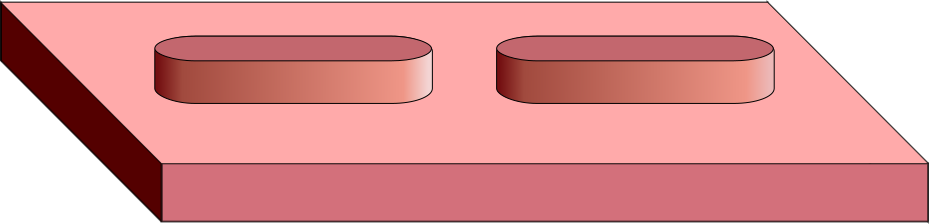
\includegraphics[width = 1.9in]{pill.pdf}
  \label{fig:pill}} \hfil
  \subfloat[]{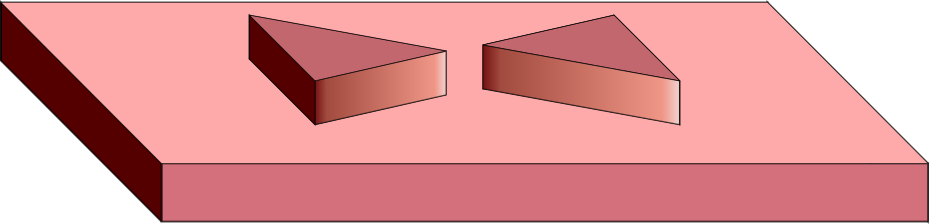
\includegraphics[width = 1.9in]{bowtie.pdf}
  \label{fig:bowtie}} \hfil
  \subfloat[]{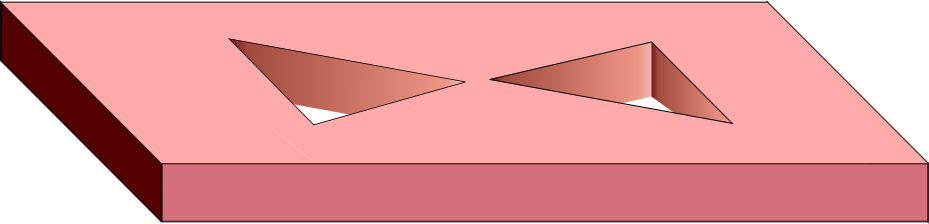
\includegraphics[width = 1.9in]{complementary_bowtie.pdf}
  \label{fig:cbowtie}}
  \caption{Common nanoantenna elements (a) dipole (b) bowtie and (c) aperture. The dipole, bowtie, and aperture antennas are typically etched on a low-loss substrate such as silicon dioxide.}
  \label{fig:antennas}
\end{figure}
%
% Fig. 1 Common nanoantenna elements (a) dipole (b) bowtie (c) aperture and (d) sphere. The dipole, bowtie, and aperture antennas are typically etched on a low loss substrate such as silicon dioxide while spheres may be mounted at the tip of a cone shaped substrate or arranged in some fashion on a flat substrate.
A majority of current research papers focus on free-space designs, but for most practical applications, nanoantennas will be etched on a substrate. The type of substrate depends on the particular application, to some extent determined by the mechanism used to excite the antenna, but for many industrial applications, cost and availability considerations have driven the move to silicon dioxide \ch{SiO2}, often described in technical papers simply as `glass'. Typical signal generation is via off-board laser light or by an on-board transmission line. Unlike classical antenna signals which can be generated at virtually any microwave carrier frequency, there are a select few frequencies where low-cost optical sources are available, although specialized lasers can operate at frequencies throughout the optical spectrum. In optical terminology the signal has traditionally been specified in wavelengths rather than frequency, however here both terms will be used. Some common wavelengths where research is being carried out are in the neighborhood of
\SI{550}, \SI{630}, and \SI{820}{\nm}. An extensive list of various laser types along with their operating frequencies can be found \cite{Weber2000}.
%
% In the optical realm, in addition to referring to `wavelength' rather than `frequency', other commonly encountered terms can at first seem odd or even incorrect to someone accustomed to working in the classical microwave domain. The term `antenna' itself is generally associated with the radiator or receiver component of a circuit, but in the nanometer regime it is also often used when describing a resonator, a device that is not intended for transmission or reception of signals. Also, the term `field intensity' is usually associated with the electric or magnetic field intensity in a microwave system, but in optics it is used to describe what an antenna engineer would refer to as the  `radiation intensity', which is power density multiplied by $r^2$.

A counter-intuitive oddity of noble metals at optical frequencies is that they are no longer perfect conductors, but rather they have some of the properties of a dielectric with, as mentioned above, a permittivity whose real part is negative. This turns out to be a remarkable advantage over dielectrics with a positive real part, due to the fact that the wavelength of the current in these metals can be much less than the wavelength of the free-space incident field. A solid nanorod still resonates around one-half wavelength of its surface current but, given an incident field frequency, one must use numerical or approximate analytical methods to determine the shorter than free-space wavelength of the antenna at resonance. While optical antennas make excellent resonators, due in part to a tightly bound plasmon current, the wavelength mismatch between air and metal, which does not exist at microwave frequencies, is a significant factor hampering their radiation and receiving properties. To understand how the radiation efficiency of an optical antenna can be improved, it is necessary to first study the unusual properties of waves on metals at optical frequencies. The essentials of optical wave propagation and radiation are presented in the following section.
%%%%%%%%%%%%%%%
%%%%%%%%%%%%%%%
%%%%%%%%%%%%%%%
\section{Electromagnetic Theory of Surface Plasmon Polaritons}
%
The physical mechanism for wave propagation at optical frequencies is very different from that of propagating waves at microwave frequencies although the mathematics for determining the wave behavior is virtually the same and can be laid out in a classical Sommerfeld integral analysis. At optical frequencies surface plasmon polaritons (SPPs), electromagnetic surface waves created by coherent charge oscillations in an electron gas in a metal, propagate at a metal-dielectric interface \cite{Ritchie1957,otto1976spectroscopy, Raether1988}. Resonant plasmonic oscillations can also occur in the confined space of nanoparticles \cite{Nie1997}. Fortunately, in most cases where optical antennas are concerned, the quantum mechanisms which create SPPs or local confined plasmons can be expressed in terms of the material properties of metals and nanoparticles, such as shape, size and permittivity \cite{Kelly2003}. Because the study of nanoantennas relies on the behavior of
plasmonic waves, it resides in the research area described as `plasmonics', a
subfield of nanophotonics \cite{Maier2005, Park2009}. In this section, some of the basic theory of SPPs will be presented to aid the reader in understanding the underlying principles that determine the behavior of nanoantennas. First, the fundamental problem of electromagnetic propagation on a planar dielectric-metal interface at optical frequencies is considered, followed by a discussion on the role played by quantum effects in determining the allowable frequency range and loss mechanisms in nano-device design. This presentation does not require an understanding of quantum mechanics, but occasionally the quantum electronics terminologies are used to describe the effects that determine the properties of the constitutive parameters at optical frequencies.
%
%
%
%
\subsection{Single Boundary Structure}
%
Assuming a metal can have a complex permittivity at optical wavelengths, the propagation constants $k_{xi}$ and $k_{zi}$ at the planar interface between dielectric and metal half-spaces, $i = 1,2$ respectively, can be found starting with expressions for transverse magnetic (TM) plane waves in these two regions as shown in Fig. \ref{fig:half_space}. The electromagnetic field expressions in region 1 where $z \ge 0$ are,
%
\begin{subequations}
  \begin{align}
    \v E_1 ={}& \left(\v{\^{x}} E_{x1}  + \v{\^{z}} E_{z1}  \right) \, \e^{ - \j \left(k_x x \,+\, k_{z1} z \right)},
    \label{eq:E_1} \\
    \v H_1 ={}& \v{\^{y}} H_{y1}  \, \e^{ - \j \left(k_x x \,+\, k_{z1} z \right)}
    \label{eq:H_1}
  \end{align}
  \label{eq:field1}%
\end{subequations}
%
\begin{figure}[t!]
  \centering
  \def\svgwidth{.75\linewidth}
  \input{figures/interface.pdf_tex}
  \caption{Dielectric and metal half-spaces with a planar boundary.}
  \label{fig:half_space}
\end{figure}
%
% Fig. 2 Dielectric and metal half-spaces with a planar boundary.
%
and in region 2 where $z \le 0$,
%
\begin{subequations}
  \begin{align}
    \v E_2 ={}& \left(\v{\^{x}} E_{x2}  + \v{\^{z}} E_{z2}  \right) \, \e^{ - \j \left(k_x x \,-\, k_{z2} z \right)},
    \label{eq:E_2} \\
    \v H_2 ={}& \v{\^{y}} H_{y2}  \, \e^{ - \j \left(k_x x \,-\, k_{z1} z \right)}.
    \label{eq:H_2}
  \end{align}
  \label{eq:field2}%
\end{subequations}
%
A positive sign is chosen for $k_{z2}$ to ensure propagation in the negative z direction. The $\Im(k_z)$ must therefore be negative in order to be bounded at infinity.

Ampere's law, $ \del\x{\v H} = -\j \O \E \,\v{E}$, applied to \eqref{eq:field1} and \eqref{eq:field2} yields the boundary conditions:
%
\begin{subequations}
  \begin{align}
    k_{z1} H_{y1} ={}& \O \E_1 E_{x1}
    \label{eq:bc1} \\
    k_{z2} H_{y2} ={}& -\O \E_2 E_{x2}
    \label{eq:bc2}
  \end{align}
  \label{eq:BC}%
\end{subequations}
%
where $\E_{1,2}$ are the permittivities of the dielectric and metal regions respectively. Since metal at optical frequencies has the behavior of a lossy dielectric, continuity of tangential electric and magnetic fields, $E_{x1} = E_{x2}$ and $H_{y1} = H_{y2}$, can be applied at the boundary along with \eqref{eq:BC}. This gives the dispersion relation for waves on the metal-air boundary:
%
\begin{equation}
  \frac{k_{z1}}{\E_1} + \frac{k_{z2}}{\E_2} = 0.
  \label{eq:dispersion}
\end{equation}
%
Helmholtz equation, $\del^2 \v E + k_i^2 \v E = 0$, where $i = 1,2$, and assuming the permeabilities of all regions are that of air, lead to the dispersion equations for the two regions,
%
\begin{equation}
  k_x^2 + k_{zi}^2 = \E_i \left( \frac{\O}{c} \right)^2 = \E_i k_0^2
  \label{eq:ks}
\end{equation}
%
where $c$ is the speed of light in air. Equations \eqref{eq:dispersion} and \eqref{eq:ks} are combined to produce the SPP propagation constant:
%
\begin{equation}
  k_x = k_0 \sqrt{\frac{\E_{r1} \E_{r2}}{\E_{r1} + \E_{r2}}}
  \label{eq:spp}
\end{equation}
%
where $k_0$ is the free-space wavenumber and the subscript $r$ is used to indicate a dielectric constant quantity. If the permittivity of the dielectric is real and that of the metal is complex, $\E_2 = \E_2' - \j \E_2''$, and $\left|\E_2' \right| \gg \E_2''$  the complex propagation constant in \eqref{eq:spp} can be expressed as \cite{Raether1988}:
%
\begin{equation}
  k_x = k_0 \left( \frac{\E_1 \E_2'}{\E_1 + \E_2'} \right)^{1/2} - \j k_0 \, \frac{\E_2''}{2 \,\E_2'^2} \left( \frac{ \E_1 \E_2'}{\E_1 + \E_2'} \right)^{3/2} = k_x' - \j k_x''.
  \label{eq:complec_kx}
\end{equation}
%
Similarly, from \eqref{eq:ks} and \eqref{eq:spp}, $k_{zi}$ becomes approximately,
%
\begin{subequations}
  \begin{align}
    k_{z1} = k_0 \left( \frac{\E_1^2}{\E_1 + \E_2'} \right)^{1/2} + \j k_0 \,  \frac{ \E_1 \E_2''}{2 \left( \E_1 + \E_2' \right)^{3/2}} = k_{z1}' + \j k_{z1}'',
    \label{eq:kz1} \\
    k_{z2} = k_0 \left( \frac{\E_2'^2}{\E_1 + \E_2'} \right)^{1/2} - \j k_0 \, \frac{\E_2''\left( 2\E_1 + \E_2' \right) }{2 \left( \E_1 + \E_2' \right)^{3/2}} = k_{z2}' - \j k_{z2}''.
    \label{eq:kz2}
  \end{align}
  \label{eq:kz}%
\end{subequations}
%
From \eqref{eq:dispersion}-\eqref{eq:kz}, some very important conclusions can be drawn regarding the nature of the two half-space materials and the properties of nano surface waves on their intersecting boundary:
%
\begin{figure}[b!]
  \centering
  \def\svgwidth{.75\linewidth}
  \input{figures/spp.pdf_tex}
  \caption{Surface plasmon propagation along a dielectric-metal boundary and exponential decay perpendicular to the boundary.}
  \label{fig:spp}
\end{figure}
% Fig. 3 Surface plasmon propagation along a dielectric-metal boundary and exponential decay perpendicular to the boundary.
%
\begin{enumerate}
  %
  \item First, if loss is neglected $(\E_2'' \simeq 0)$, a valid assumption for noble metals over significant segments of the optical range so that the permittivities of both regions are real, the equality in \eqref{eq:dispersion} will not hold if these permittivities are both positive or both negative. But, if the permittivity in the dielectric region $1$ is positive, $\E_1 > 0$, and the real part of the permittivity in the metal region $2$ is negative, $\E_2' < 0$, then it is possible to satisfy \eqref{eq:dispersion}.
  %
  \item	Nevertheless, a wave still cannot exist if the term under the square root in \eqref{eq:spp} is negative because this would lead to a totally complex $k_x$, which would mean the fields in \eqref{eq:field1} and \eqref{eq:field2} will exponentially grow or decay rather than propagate along the boundary. However, if
  %
  \begin{equation}
    \E_1 > 0, \quad		 \E_2' < 0, \quad   \text{and}  \quad \left| \E_2' \right| > \E_1,
    \label{eq:conditions}
  \end{equation}
  %
  then the term under the square root in \eqref{eq:spp} is positive and propagation of a wave at the boundary is assured. This condition \eqref{eq:conditions} causes the signs of the terms under the square roots in \eqref{eq:kz} to be negative, but \eqref{eq:dispersion} will still hold as long as same sign for $\sqrt{-1}$ is chosen for both square roots.
  %
  \item	If the conditions in \eqref{eq:conditions} are met then from \eqref{eq:spp}, $k_x > k_0$ and therefore $k_z$ in \eqref{eq:ks} must be complex. According to \eqref{eq:field1} and \eqref{eq:field2}, this results in exponential decay of the field away from the boundary in both the positive and negative z-directions as long as $\sqrt{-1} = -\j$ is chosen for the square root terms in \eqref{eq:kz}. Exponential decay of the plasmon surface wave into the dielectric and metal is illustrated in Fig. \ref{fig:spp}.
  %
  \item	According to Snell's law, the component of the wavenumber $k_x$ tangential to the boundary is the same in both mediums. If medium 1 is air, the x-component of a plane wave incident upon the boundary at an angle $\theta$ from normal is $k_{x1} = k_0 \sin \theta$, which is less than $k_0$. However, according to \eqref{eq:spp} and \eqref{eq:conditions} surface plasmons cannot exist unless $k_x > k_0$. Therefore, surface plasmons cannot be excited by shining light on a flat metal surface.
  %
  \item	From \eqref{eq:complec_kx}, the velocity of a surface plasmon wave on a planar boundary is:
  %
  \begin{equation}
    v_{sp} = \frac{\O}{k_x'} = c \left( \frac{\E_1 + \E_2'}{\E_1 \E_2'} \right)^{1/2}
    \label{eq:velocity}
  \end{equation}
  %
  and its wavelength is:
  %
  \begin{equation}
    \lambda_{sp} = \frac{2 \pi}{k_x'} = \left( \frac{\E_1 + \E_2'}{\E_1 \E_2'} \right)^{1/2}
    \label{eq:wavelength}
  \end{equation}
  %
  \item	The exponential decay of a plasmon along its propagation direction is determined by the second term in \eqref{eq:complec_kx}. The `propagation length' of a plasmon wave is the distance $x = L$ at which the wave decays to   $1/e$ of its initial value. The plasmon propagation length on a planar surface is therefore:
  %
  \begin{equation}
    L = \frac{1}{k_x'} = \frac{2 \,\E_2'^2}{k_0 \,\E_2''} \left( \frac{\E_1 + \E_2'}{\E_1 \E_2'} \right)^{1/2}
    \label{eq:plength}
  \end{equation}
  %
  \item	If the conditions in \eqref{eq:conditions} hold, the second term on the right hand side in \eqref{eq:kz1} and \eqref{eq:kz2} are small so, neglecting these terms, perpendicular to the boundary the $1/e$ decay distance into the dielectric is \cite{Raether1988}:
  %
  \begin{equation}
    z_1 = \left| \frac{1}{k_{z1}'} \right| = \frac{1}{k_0} \left| \frac{2 \, (\E_2')^2}{k_0 \,\E_2''} \left( \frac{\E_1 + \E_2'}{\E_1^2} \right)^{1/2} \right|
    \label{eq:decay_dielectric}
  \end{equation}
  %
  and,
  \begin{equation}
    z_2 = \left| \frac{1}{k_{z2}'} \right| = \frac{1}{k_0} \left| \frac{2 \, (\E_2')^2}{k_0 \,\E_2''} \left( \frac{\E_1 + \E_2'}{\E_2'^2} \right)^{1/2} \right|
    \label{eq:decay_metal}
  \end{equation}
  %
  into the metal.
  \item	Power and energy relationships can be found by assuming a value for the magnetic field amplitude and by using Ampere's law to determine the electric field.
\end{enumerate}
%
The conditions described in \eqref{eq:conditions} are met by noble metals in air for the optical and near-infrared ranges in the case of a TM polarized wave. A similar analysis will show that a transverse electric (TE) polarized wave cannot exist at a dielectric-metal boundary.

In practical applications, one should take care in the selection of the metal to be used in a nanoantenna design. Some metals, such as silver, tend to develop an oxidation layer, which can severely decrease propagation length and increase the antenna impedance. For a more detailed discussion concerning the effect of a silver sulfide oxidation layer on a silver substrate plasmon wave, the reader is referred to \cite{Nevels2014}.
%
Fig. \ref{fig:plength} shows the propagation length as a function of wavelength for three metals, gold, silver and aluminum \cite{9783540339199}. The practitioner is cautioned that although the propagation length of a surface plasmon does increase as frequency decreases, the analysis leading to this figure is based on an idealization of the physical problem. Here, a pure wave propagation condition was assumed in the formulation of equations \eqref{eq:field1} and \eqref{eq:field2}. In the practical case, a source such as the feed point of an antenna, must be included in the problem formulation. If the source is included, one sees that as the frequency decreases, less energy is transferred into the surface plasmon wave and more into the space wave; the field that is radiated directly into space from the source point. In the far infrared frequency range, the surface plasmon essentially ceases to exist. Plasmon wave behavior is discussed in more detail in the section of this chapter concerning aperture antennas.
%
\begin{figure}[t!]
  \centering
  {\includegraphics[width = .5\linewidth]{generate_fig4.tikz}}
  \caption{Propagation length of a surface plasmon propagating along the interface between a dielectric (refractive index 1.32) and a metal as a function of wavelength calculated for gold (Au), silver (Ag), and aluminum (Al).}
  \label{fig:plength}
\end{figure}
% Fig. 4 Propagation length of a surface plasmon propagating along the interface between a dielectric (refractive index 1.32) and a metal as a function of wavelength calculated for gold (Au), silver (Ag), and aluminum (Al).
%
%%%%%%%%%%%%%%%
%%%%%%%%%%%%%%%
%%%%%%%%%%%%%%%
\section{Quantum effects}
%
The above analysis considers only the classical electromagnetic aspects of propagation on a dielectric metal boundary. However, quantum mechanical effects inherent in metals and dielectrics enter the picture through the permittivity, thereby determining its value as well as the frequency range over which SPPs can propagate. Essentially, quantum processes reveal the frequency range over which the metal has a permittivity with a negative real part and where losses begin to have a serious effect on wave propagation within that frequency range. In the following, the influence of plasma resonance and atomic collisions on SPP propagation are briefly explored.  Although the properties described below are best understood using quantum mechanics, the mathematics below is classical, primarily developed by concatenating harmonic oscillator models. However, the differences in the results of the two theories is small, allowing classical electromagnetic calculations without the necessity of delving into quantum theory.
Free electrons can exist near the top of the energy band distribution in a metal. The interaction of these electrons with photons and the long-range Coulomb force of atoms create an electron oscillation known as a plasmon. Taking these effects into account, the dielectric function of metal can be expressed in terms of the Drude model \cite{MaxBorn2002}:
%
\begin{equation}
  \E(\O) = 1 - \frac{\O_p^2}{\O(\O  - \j \nu)} = \left(1 - \frac{\O_p^2}{\O^2 + \nu^2} \right) - \j \frac{\nu \, \O_p^2}{\O (\O^2 + \nu^2)} = \E_r - \j \E_i
  \label{eq:drude}
\end{equation}
%
where $\nu = 1/\tau$ is the collision frequency, $\tau$ is the scattering time between collisions, and $\O_p$ is the plasma frequency that is expressed as:
%
\begin{equation}
  \O_p = \sqrt{\frac{N e^2}{\E_0 m_e}}
  \label{eq:plasma_f}
\end{equation}
%
in which $e$ and $m_e$ are the electron charge and mass respectively and $N$ is the concentration of free electrons. Plasma frequencies for metals are in the visible and ultraviolet ranges. Typical values of plasma and collision frequencies are $\O_p = \SI{.23e12}{\Hz}$ and
$\nu = \SI{5.51e12}{\Hz}$ for gold and $\O_p = \SI{.21e16}{\Hz}$ and $\nu = \SI{4.45e12}{\Hz}$ for silver, however impurities and other factors can affect these numbers so the literature does not have a unique set of values for these parameters. A comprehensive list of plasma and collision frequencies published by a variety of researchers for gold, silver and other noble metals can be found at \cite{Moroz2010}.

Collisions are primarily between electrons and relatively large lattice vibrations (phonons), so for most metals at room temperature  $\nu \ll \O_p $ \cite{Bohren1998}, which reduces \eqref{eq:drude} to approximately:
%
\begin{equation}
  \E(\O) \simeq 1 - \frac{\O_p^2}{\O^2}
  \label{eq:drude_approx}
\end{equation}
%
This important expression shows that when $\O < \O_p$, then $\E(\O) < 0$  which in part satisfies the conditions in \eqref{eq:conditions}. Therefore, surface plasmon polaritons can only exist below the plasma frequency. Equation \eqref{eq:drude_approx} substituted into \eqref{eq:spp} gives a simplified Drude model for the plasmon wavenumber:
%
\begin{equation}
  k_x \simeq k_1 \left( \frac{\O^2 - \O_p^2}{\O^2 \E_{r1} + (\O^2 - \O_p^2)} \right)^{1/2}
  \label{eq:kx_approx}
\end{equation}
%

The Drude model in the form given in \eqref{eq:drude} is widely used in nanoantenna analytical and numerical calculations for determining the permittivity, and therefore the propagation constant, of the plasmon polariton of noble metals. However, this free electron model fails at frequencies higher than about \SI{850}{\tera\Hz} \cite{Archambault2009}, due to bound charge effects, and must be modified by incorporating additional terms \cite{Bohren1998}. This becomes a tedious process but reasonable accuracy can be achieved. Another option, preferred by the authors, is to use measured data \cite{Lynch1997} with a partial fraction fit \cite{Michalski2013}. Fig. \ref{fig:permittivity} shows the dielectric function for gold and silver over the frequency range from \SI{.5}{\electronvolt}\texttildelow \SI{120}{\THz} to \SI{6.5}{\electronvolt}\texttildelow \SI{1.57}{\peta \Hz} obtained from measured data via a partial fraction fit. The solid lines are the
partial fraction fit for the real part $\E'$, and the dashed lines are for the imaginary part $\E''$, of the dielectric function.
%
\begin{figure}[t!]
  \centering
  \subfloat[]{\includegraphics[width = .5\linewidth]{ep_gold.tikz}
  \label{fig:ep_gold}} \\
  \subfloat[]{\includegraphics[width = .5\linewidth]{ep_silver.tikz}
  \label{fig:ep_silver}}
  \caption{Dielectric function for (a) Gold and (b) Silver as a function of  photon energy $E = hf$ where $f$ is frequency and $h = \SI{6.626e34} {kg.m^{2}/s}$ is Planck's constant. The solid lines are the partial fraction fit for $\E'$ and the dashed line is for $\E''$. The circles and squares are from measured data originally listed in \cite{Johnson1972}}
  \label{fig:permittivity}
\end{figure}
% Fig. 5 Dielectric function for (a) Silver and (b) Gold as a function of photon energy where f is frequency and   m2 kg/s is Planck's constant. The solid lines are the partial fraction fit for  and the dashed line is for   . The circles and squares are from measured data originally supplied by (Johnson and Christy 1972).
%

The significance of the data in Fig. \ref{fig:permittivity} becomes clearer in Fig. \ref{fig:dispersion} where the surface plasmon dispersion curve for frequency versus the propagation $k_x'$, attenuation $k_x''$, and constants at an air-silver boundary are plotted. The lower part of the curve is the non-radiative surface plasmon region followed above by an anomalous dispersion region and above that a Brewster mode radiative region. The slanted dashed line is the free-space light line $k_0 = \O/c$. The Brewster mode portion of the dispersion curve is in the fast wave region to the left of the light line. It is the locus of the values of $k_x$ of the plane wave incident on the boundary at the Brewster angle. These waves do not set up a surface wave, but rather carry their power directly into the metal without reflection. Below the Brewster mode section is a region of anomalous dispersion, often described in the literature as `backbending', which has a group velocity that is virtually zero, and is accompanied by high loss.
%
\begin{figure}[t!]
  \centering
  {\includegraphics[width = .5\linewidth]{disp_silver.tikz}}
  \caption{SPP dispersion curve for $\O$ versus $\Re (k_x)$ and $\Im (k_x)$ for an glass-silver interface. The lower part of the curve is the non-radiative surface plasmon region which is capped by a high-loss backbending region, and a Brewster mode radiative region above}
  \label{fig:dispersion}
\end{figure}
% Fig. 6 SPP dispersion curve for   versus   and   for an air-silver interface. The lower part of the curve is the non-radiative surface plasmon region which is capped by a high loss backbending region, and a Brewster mode radiative region above.
%

The surface plasmon portion of the dispersion curve is of primary importance to nanoantenna design. The plasmon region lies to the right of the light line and therefore, it is a slow wave since the phase velocity here is less than the speed of light. Because surface plasmons have a shorter wavelength than light they are prevented from radiating from a flat planar surface. Of particular significance is the decreasing slope of the dispersion curve, tending toward horizontal near where it joins the anomalous dispersion segment. In the plasmon region the surface plasmon propagation constant increases dramatically with a small increase in frequency. The horizontal dashed line at \SI{380}{\nm} intersects the light line at approximately $k_0 = \SI{17}{\radian \per \micm}$ while at the same wavelength $k_x' = \SI{21}{\radian \per \micm}$, which means the surface plasmon wavelength can be much less than the free-space wavelength. Therefore, a resonant half-wavelength nano-dipole antenna can be much smaller than a half-wavelength measured in air at the same frequency. As the plasmon wavelength decreases near the anomalous dispersion region, the propagation constant approaches a limiting value. The Drude model provides the estimate for this limiting frequency
%
\begin{equation}
  \O_{sp} \simeq \O_p/\sqrt{1 + \E_{r1}},
  \label{eq:apprx_plasma_freq}
\end{equation}
%
obtained by setting the denominator in \eqref{eq:kx_approx} equal to zero, which is equivalent to assuming the propagation constant in \eqref{eq:kx_approx} approaches infinity. This is not what happens to the propagation constant, as can be seen in Fig. \ref{fig:dispersion} where real data is used, but it does provide a reasonable estimate of the limiting frequency. nanoantennas must be designed to operate below this frequency, thereby avoiding a group velocity approaching zero and dramatically increased losses.

Although several key aspects of wave propagation on nano-structures have been presented here, all analysis has been performed assuming propagation is on a surface between two half spaces. However, most nanoantennas have air above and are etched in a noble metal, such as gold, on a dielectric substrate, such as silicon dioxide. The metal antenna, therefore lies between two different materials. nanoantennas are typically excited at a corner or edge where both upper and lower surfaces are exposed to the incoming electromagnetic field. Because the plasmon propagation constant \eqref{eq:complec_kx} is a function of the permittivity in the regions above and below an interface, it will be helpful to understand how different phase velocities \eqref{eq:velocity} and wavelengths \eqref{eq:wavelength} on the two sides of a nanoantenna will affect its performance. This issue is briefly addressed in the following paragraphs.
%%%%%%%%%%%%%%%
%%%%%%%%%%%%%%%
%%%%%%%%%%%%%%%
%%%%%%%%%%%%%%%
%%%%%%%%%%%%%%%
%%%%%%%%%%%%%%%
\section{Two Boundary Structures}
%
Surface plasmon polaritons on a metal film have properties that do not exist on an interface between metal-dielectric half spaces. To analyze the mode configuration on a metal strip of thickness $t$, consider the configuration shown in Fig. \ref{fig:3layer} where the dielectrics are assumed to extend from the surface of the metal to infinity and possess different permittivities, $\E_1$ and $\E_2$. The permittivity of the metal is $\E_m$ and all three regions have the permeability of free-space. The waves in each region are assumed to be TM polarized with a magnetic field component in the y-direction in each region given by:
%
\begin{figure}[b!]
  \centering
  \def\svgwidth{.5\linewidth}
  \input{figures/three_layer.pdf_tex}
  \caption{Thin metallic film between two dielectric regions with different permittivities.}
  \label{fig:3layer}
\end{figure}
% Fig. 7 Thin metallic film between two dielectric regions with different permittivities.
%
\begin{subequations}
  \begin{align}
    \v H_1 ={}& \v{\^{y}} \,H_{y1} \, \e^{ -\A_{z1}z \,- \j k_x x}, \qquad	 		\text{dielectric region 1} (z \ge t)
    \label{eq:H1_3layer}\\
    \v H_m ={}& \v{\^{y}} \,\left( H_{ya}\, \e^{ +\A_{zm}z} + H_{yb}\, \e^{ -\A_{zm}z} \right) \, \e^{ - \j k_x x}, \qquad	 		\text{metal region m} (0 \le z \le t)
    \label{eq:Hm_3layer}\\
    \v H_2 ={}& \v{\^{y}} \,H_{y2} \, \e^{ -\A_{z3}z \, - \j k_x x}, \qquad	 		\text{dielectric region 2} (z \le 0)
    \label{eq:H2_3layer}
  \end{align}
  \label{eq:H_3layer}%
\end{subequations}
%
where the dispersion relations for the three regions are,
%
\begin{equation}
  \A_{zi}^2 = -k_{zi}^2 = k_x^2 - k_0^2 \E_i, \qquad	  \text{for} \,
  i=1,2,m
  \label{eq:3_layer_disp}
\end{equation}
%
and the boundary conditions satisfied by $\v H_m$ at each interface are:
%
\begin{subequations}
  \begin{align}
    {H_{ym}} ={}& {H_{yi}}
    \label{eq:bc1_3layer}\\
    \frac{1}{\E_m}\pdv{H_{ym}}{z}  ={}& \frac{1}{\E_i}\pdv{H_{yi}}{z}
    \label{eq:bc2_3layer}
  \end{align}
  \label{eq:bc_3layer}%
\end{subequations}
%
where $i = 1,2$. Each of these conditions are applied to \eqref{eq:H_3layer} at each boundary yielding a set of four homogeneous linear equations which can be combined to produce:
%
\begin{subequations}
  \begin{align}
    \frac{H_{yb}}{H_{ya}} ={}& \ddfrac{\left(\frac{\E_2 \,\A_{zm}}{\E_m \,\A_{z2}} - 1 \right)}   {\left(\frac{\E_2 \,\A_{zm}}{\E_m \,\A_{z2}} + 1 \right)}
    \label{eq:homo1_3layer}\\
    \frac{H_{yb} \, \e^{-2 \A_{zm}t}}{H_{ya}} ={}& \ddfrac{\left(\frac{\E_1 \,\A_{zm}}{\E_m \,\A_{z1}} + 1 \right)}   {\left(\frac{\E_1 \,\A_{zm}}{\E_m \,\A_{z1}} - 1 \right)}
    \label{eq:homo2_3layer}
  \end{align}
  \label{eq:homo_3layer}%
\end{subequations}
%
The equations in \eqref{eq:homo_3layer} are equated to produce the three dispersion relation:
%
\begin{equation}
  \left(\frac{\E_m \,\A_{z1}}{\E_1 \,\A_{zm}} + 1 \right) \left(\frac{\E_m \,\A_{z2}}{\E_2 \,\A_{zm}} + 1 \right) = \left(\frac{\E_m \,\A_{z1}}{\E_1 \,\A_{zm}} - 1 \right) \left(\frac{\E_m \,\A_{z2}}{\E_2 \,\A_{zm}} - 1 \right) \, \e^{-2\A_{zm}t}
  \label{eq:3layer_dispersion}
\end{equation}
%
for the metal layer sandwiched between two different dielectrics. Equation \eqref{eq:3layer_dispersion} can be verified by allowing the metal thickness to become large, $\A_{zm}t \rightarrow \inf$, in which case the right hand side goes to zero. This yields a pair of equations:
%
\begin{subequations}
  \begin{align}
    \frac{\E_m \A_{z1}}{\E_1 \,\A_{zm}} + 1 ={}& 0
    \label{eq:simplified1_3layer_to2layer}\\
    \frac{\E_m \A_{z2}}{\E_2 \,\A_{zm}} + 1 ={}& 0,
    \label{eq:simplified2_3layer_to2layer}
  \end{align}
  \label{eq:simplified_3layer_to2layer}%
\end{subequations}
%
recognized from \eqref{eq:dispersion} to be the dispersion relations for surface plasmon polaritons at the boundaries between two individual dielectric-metal half-spaces.

If $\E_1$ and $\E_2$ are positive and $\E_m < 0$, the right hand side of \eqref{eq:3layer_dispersion} is positive, which means the left hand side must also be positive. This is possible if,
$\left( \frac{\E_m \,\A_{z1}}{\E_1 \,\A_{zm}} + 1 \right)$ and
$\left( \frac{\E_m \,\A_{z2}}{\E_2 \,\A_{zm}} + 1 \right)$ are both positive or both negative. Under the assumption that both are negative, that
$ \E_1 > \E_2 $, and $\left| \E_m \right| > \E_1$  the characteristic equation \eqref{eq:3layer_dispersion} becomes \cite{Durach_2007},
%
\begin{equation}
  \A_{zm}t = \coth ^{-1} \left( \frac{\left| \E_m \right|\A_{z1}}{\E_1 \,\A_{zm}} \right) + \coth ^{-1} \left( \frac{\left| \E_m \right|\A_{z2}}{\E_2 \,\A_{zm}} \right).
  \label{eq:3layer_xtic_coth}
\end{equation}
%
Similarly, assuming that both expressions in brackets on the left hand side of \eqref{eq:3layer_dispersion} are positive and
$\left| \E_m  \right| < \frac{\E_1 \E_2}{\E_1 - \E_2}$  the characteristic equation becomes \cite{Durach_2007},
%
\begin{equation}
  \A_{zm} t = \tanh^{-1} \left( \frac{\left| \E_m \right| \A_{z1}}{\E_1 \,\A_{zm}} \right) + \tanh^{-1} \left( \frac{\left| \E_m \right| \A_{z2}}{\E_2 \,\A_{zm}} \right).
  \label{eq:3layer_xtic_tanh}
\end{equation}
%
Equations \eqref{eq:3_layer_disp} together with \eqref{eq:3layer_xtic_coth} or \eqref{eq:3layer_xtic_tanh} can be used to solve for the wavenumbers in the even and odd mode cases, referring respectively to the symmetric or asymmetric form of the tangential (z-directed) component of the electric field about the center of the metal layer \cite{Burke1986}.

When the metal layer is thick, the waves on the two sides of the metal slab do not interact, as indicated in \eqref{eq:simplified_3layer_to2layer}. However, as the slab becomes thinner the electromagnetic fields on the two sides do interact and the frequency splits into a low frequency even mode \eqref{eq:3layer_xtic_coth} and a higher frequency odd mode \eqref{eq:3layer_xtic_tanh}. Although the tangential electric field is not entirely symmetric in the metal region when $\E_1 \ne \E_2$, more of the field lies inside the metal in the even mode case \eqref{eq:3layer_xtic_coth} than it does in the basically asymmetric odd mode case \eqref{eq:3layer_xtic_tanh}. As the metal layer becomes thinner, the damping of the odd mode decreases, approximately as the square of the thickness, allowing this mode to travel a greater distance than a plasmon polariton on the interface between two half spaces. However, the basically symmetric mode damping increases with decreasing thickness, allowing propagation distances one or two orders of magnitude greater than those of thick metal construction
\cite{Sarid1981}. The physical reason attributed to this phenomena is that in the asymmetric case, where the null is in the center of the metal, more of the field resides outside as the thickness of the metal decreases therefore, lessening the presence of the tangential electric field in the metal thereby reducing Joule heat which in turn decreases the electron collision rate resulting in less damping of the wave. This analysis suggests that the efficiency of an optical antenna can be improved by decreasing the thickness of the metallic material with which it is constructed and operating in the higher odd mode frequency range.

When the metal width is finite and the environment is symmetric $(\E_1 = \E_2)$, there are four fundamental modes and a number of higher order modes. These modes can be classified according to the cross-sectional width and thickness, similar to a rectangular waveguide and will become successively cut off as the thickness decreases leaving one Gaussian like mode. Efficient optical fiber coupling to this plasmonic mode in a metal guide has been demonstrated \cite{Berini2000}, raising the possibility of similar coupling between optical antennas and metal strip plasmonic waveguides designed with the appropriate width and thickness so as to operate in this particular mode. Closer to the nanoantenna case, in an asymmetric environment $(\E_1 \ne \E_2)$ there is no purely TM mode. It has been shown that modes in this case can change their symmetry properties with changes in both transverse directions, width and thickness, and that all modes show a cutoff height that increases both with decreasing width and increasing dielectric mismatch
between the sub- and superstrate \cite{Berini2000,Berini2001}. Unfortunately, this includes air-metal-glass configurations commonly used in the design of optical antennas and waveguides. Thus the complicated spatial profiles shown in modes in an asymmetric environment prohibit efficient excitation techniques \cite{Maier2005,Yang1991}.

In this section it has been shown that in the optical frequency range electromagnetic wave propagation, which is via a surface plasmon polariton, can take place on an air-dielectric boundary if one of the two materials has a dielectric constant with a negative real part obeying the conditions in \eqref{eq:conditions}. The dispersion equation for this wave is given in \eqref{eq:spp} and presented graphically in Fig. \ref{fig:dispersion}, which shows that a surface plasmon is a slow wave, i.e. slower than the speed of light in the dielectric medium. The Drude model, which is relatively accurate below, and not too close to, the plasma frequency $\O_p$ and useful for analytical calculations, was given in \eqref{eq:drude}. This model, or its approximation in \eqref{eq:drude_approx}, is commonly used to obtain approximate velocity \eqref{eq:velocity}, wavelength \eqref{eq:wavelength}, propagation distance \eqref{eq:plength}, and exponential decay distance away from the boundary \eqref{eq:decay_dielectric} and
\eqref{eq:decay_metal} of the plasmon wave. It also provides an estimate of maximum frequency \eqref{eq:apprx_plasma_freq} at which a plasmon wave can propagate. Although Fig. \ref{fig:dispersion} shows that the surface plasmon wavelength can be much less than the free-space wavelength, close to the maximum frequency the plasmon wave will experience severe attenuation.

Because optical antennas are operated in a frequency range which is at the overlapping boundary between electromagnetic and quantum theories, in the paragraphs above, some of the quantum justification for the unusual behavior of materials in the near infrared and optical domains has been presented. This discussion was then followed by an asymmetric two boundary case development of the dispersion equations modeling a typical optical antenna structure in cross-section, showing that the interaction between the plasmon waves on the two boundaries breaks into symmetric and asymmetric modes, \eqref{eq:3layer_xtic_coth} and \eqref{eq:3layer_xtic_tanh}. The symmetric mode is preferred when coupling to another device and the asymmetric mode is preferred for long distance propagation in a plasmon waveguide. This section then concluded with a discussion of the finite width metal guide that has been shown to have a complicated mode structure, hampering efforts to obtain a mathematical expression for impedance matching. Current attempts at obtaining a mathematical model and along with design methods that improve impedance matching and enhance optical antenna radiation will be covered in the individual antenna discussions that follow.
%%%%%%%%%%%%%%%
%%%%%%%%%%%%%%%
%%%%%%%%%%%%%%%
%%%%%%%%%%%%%%%
%%%%%%%%%%%%%%%
%%%%%%%%%%%%%%%
\section{Design of Optical Antennas}
%
The plasmonic nature of nanoantenna operation prevents the designer from describing antenna performance with formulas that have been developed over many decades at microwave and lower frequencies. Dielectric properties of metals are only one factor preventing a direct correspondence between established antenna theory and actual optical antenna operation. A traditional antenna concept that the wave vector for the current is the same as the free-space wave vector must be abandoned, dispersion effects must be accounted for and losses not generally expected in a microwave frequency  `perfect conductor' become dependent on the size and shape of the antenna.
The optical antenna, although not a traditional perfect conductor, cannot be analyzed as though it is a pure dielectric rod as would be the case for an optical fiber. But even if an optical antenna could be modeled as a pure dielectric, the tips of a rod represent the famous unsolved dielectric wedge problem. As described above, the fast wave current on a perfect conductor must be replaced by a slow wave plasmon current tightly coupled to the antenna surface. Radiation on an optical dipole still occurs at the tips of the rods and can still be viewed as current induced. The primary difficulty that must be faced when attempting an analytical analysis is that for practical reasons the design requires placing the antenna on an interface between a dielectric below, such as a silicon dioxide substrate, and air above. Although numerical techniques can be used to accurately analyze the characteristics of the structure, similar to microstrip patch antennas, no exact analytical methods are available. Analytical approximations and numerical attempts to obtain the basic characteristics of an optical antenna, the resonant frequency, input impedance, gain, directivity and efficiency, are presented in this section.
%%%
%%%
%%%
\subsection{Dipole and Patch Antennas}
%
Size and shape can affect the design frequency of an optical antenna in ways not typically expected in microwave frequency antenna engineering. For example a rectangular microstrip patch is expected to resonate when the incident field is polarized in the direction of the $\lambda/2$ dimension of the patch, while the transverse dimension is flexibly left to something greater or less than $\lambda/2$. However, as shown in Fig. \ref{fig:simulation} both the width and length of a metal plate must be considered in designing an optical antenna. A narrow nanodipole resonating at a particular frequency, as shown in Fig. \ref{fig:nitin_dipole}, does not maintain resonance
%
\begin{figure}[b!]
  \centering
  \def\svgwidth{.75\linewidth}
  \input{figures/dipoles_nitin.pdf_tex}
  \caption{A gold dipole residing over a glass substrate.}
  \label{fig:nitin_dipole}
\end{figure}
%
\begin{figure}[t!]
  \centering
  \subfloat[]{\includegraphics[height = 2.7in]{generate_fig8c.tikz}
  \label{fig:sim_hi}}\\
  \centering
  \subfloat[]{\includegraphics[height = 1.9in]{fig8_a.png}
  \label{fig:narrow}} \hfil
  \subfloat[]{\includegraphics[height = 1.9in]{fig8_d.png}
  \label{fig:wide}} \hfil
  \caption{(a) Maximum enhancement of a gold nanodipole excited at \SI{550}{\nm} (b) narrow and (c) wide profile. A narrow structure does not maintain resonance when widened without also changing its length.}
  \label{fig:simulation}
\end{figure}
% Fig. 8 Maximum enhancement of a gold nanodipole excited at 550 nm (a) narrow and (b) wide profile. A narrow structure does not maintain resonance when widened without also changing its length.
%
when widened. However, the first resonance can be regained by changing both the length and width of the dipole as shown in Fig. \ref{fig:wide}. The mechanism causing this phenomena has to do with the manner in which surface plasmons are excited. The incident wave with a free-space wavenumber transfers energy into the plasmon wave having a much larger wavenumber at locations where the interaction between the incident wave and the antenna produce the largest concentration of higher order modes, which will couple energy into the plasmon mode. This interaction is primarily seen on the corners of the dipole in Fig. \ref{fig:wide}. Similar to plane waves in a waveguide, plasmon waves fan out from the corners taking a circuitous route bouncing from the edges of the plate before phase matching produces a resonance condition. Further complicating the picture is the chemical potential and the `lighting rod' effect whereby opposite charges form a high concentration of the field across the antenna
center gap. However, plasmons in the narrower dipole, Fig. \ref{fig:narrow}, follow a shorter, more direct route to resonance than does the plasmon wave on the wider dipole Fig. \ref{fig:wide} thereby experiencing less attenuation and ultimately creating a region of higher field enhancement in the gap than does the wide dipole. Fig. \ref{fig:sim_hi} shows that as the dipole widens the resonant frequency shifts and the enhancement decreases.  Enhancement is defined as the ratio of the total to the incident electric field in the gap region, although in some publications this ratio is squared and therefore, described as intensity enhancement.

The behavior of the narrower dipole shown in Fig. \ref{fig:narrow} is more closely aligned with what one would expect at microwave frequencies whereby increasing the length of each nanorod in plasmon half-wavelength intervals will produce successive resonance and antiresonance in the gap input impedance. Notice that the total length of the dipole is a full plasmon wavelength $\lambda_p$ plus the gap separation distance, as opposed to the typical $\lambda_0/2$ dipole first resonance of a perfectly conducting microwave antenna with a negligible gap width. In terms of plasmon wavelengths, a first resonance does occur in an isolated $\lambda_p/2$ nanorod or a vertical $\lambda_p/4$ nanorod on a metal substrate \cite{Taminiau2007}.

Although an exact determination of the plasmonic wavelength in a dielectric nanorod is not mathematically feasible, an effective wavelength $\lambda_{eff}$ based on the assumption that the antenna is a thin dielectric cylinder operating in the $\mathrm{TM}_0$ cylindrical waveguide mode has been derived in \cite{Novotny2007}. The antenna is immersed in a material with dielectric constant $\E_s$, and a Drude dielectric function is used to describe the metal rod material. The apparent increase in the antenna length at the rod ends is accounted for by an additional reactance term. This scaling law is:
%
\begin{equation}
  \lambda_{eff} = n_1 + n_2\left( \frac{\lambda}{\lambda_p} \right)
  \label{eq:lambda_eff}
\end{equation}
%
where $\lambda$ is the wavelength of the external region, $\lambda_p$ is the metal plasma wavelength, and $n_1$, $n_2$ coefficients with dimensions of length that depend on antenna geometry and static dielectric properties, are
%
\begin{subequations}
  \begin{align}
    n_1 ={}& 2\, \pi\, R \left[ 13.74 - 0.12 \frac{\E_\inf + 141.04\, \E_s}{\E_s} - 2\pi \right]
    \label{eq:n1}\\
    n_2 ={}& 0.24\, \pi\, R \frac{\sqrt{\E_\inf + 141.04 \, \E_s}}{\E_s}.
    \label{eq:n2}
  \end{align}
  \label{eq:ns}%
\end{subequations}
%
Here $R$ is the radius of the cylinder, and $\E_{\inf}$ is the dielectric constant correction in the Drude formula for $\O \gg \O_p$. For gold $\E_\inf \simeq 11$, $\lambda_p = \SI{138}{\nm}$ and for silver $\E_\inf \simeq 3.5$, $\lambda_p = \SI{135}{\nm}$ \cite{Novotny2007}.

In the case of an optical patch or dipole antenna it is necessary to account for a phase shift acquired by the surface plasmon polariton upon reflection at rod, strip, or gap terminations. The resonance wavelength $\lambda$ of metal strip resonators of thickness $t$ and width $w$ are determined approximately by \cite{Sondergaard2007}:
%
\begin{equation}
  w \frac{2 \pi}{\lambda} n_{slow} = m\pi  - \phi
  \label{eq:resonant_lambda}
\end{equation}
%
where $n_{slow}$ is the real part of the mode index of surface plasmon polaritons propagating in a metal film with the same thickness $t$ as the strip, $m = 1,2,3,\dotsc $ is the order of the resonance, and $\phi$ is the phase of the reflection coefficient at strip terminations. For a symmetric structure where $\E_d = \E_1 = \E_2$, once $t$ and $\E_m$ are selected and the phase shift $\phi$ is determined, $n_{slow}$ can be obtained from \eqref{eq:3_layer_disp} and \eqref{eq:simplified_3layer_to2layer} or for thin strips, one can use the approximation \cite{Sondergaard2008}:
%
\begin{equation}
  n_{slow} \simeq \sqrt {n_d^2 + \frac{4 \, n_d^4}{k_0^2 \, t^2 \, n_m^4}}
  \label{eq:n_approx}
\end{equation}
%
where $n_d$ and $n_m$ are the indices of refraction of the dielectric and metal and $k_0 = 2 \pi /\lambda$. The wavelength of the slow surface plasmon polariton is then given by $\lambda_{slow} = \lambda/ n_{slow}$.

Analytical models are preferable because clear trends in antenna performance can be seen by adjusting mathematical parameters that represent physical quantities such as the antenna width or length and the excitation frequency. On the other hand, numerical techniques can provide both the accuracy and flexibility needed to model complex antenna structures. However, purely mathematical solutions can become clouded with long complex expressions and special functions while a purely numerical analysis provided by the powerful commercial codes that have become available these last few years, while furnishing useful visual data in terms of graphs and charts, do not always provide a way to understand the multifaceted interaction between the variables of an antenna system. Recently a compromise approach for optical antennas has been advanced, advocated primarily by Engheta and Alù \cite{Engheta2005,Alu2007,Zhao2011,9781107014145}, whereby the antenna and field excitation are replaced by an equivalent lumped circuit model based on
numerical analysis data. The basic model, shown in Fig. \ref{fig:alu_circuit}, is centered on a Thévenin equivalent circuit for the antenna with a capacitance accounting for a non-negligible gap
impedance $Z_g$ along with the intrinsic impedance $Z_a$ of the dipole. The parallel combination of these two impedances forms the input impedance of the circuit. The input impedance is calculated, by driving the antenna at the gap with an arbitrary source voltage $V_g$ and calculating, with full-wave simulations, the displacement current $I_g$ flowing across the arms at the terminals in the region of the gap $Z_{in} = V_g / I_g$.

The intrinsic antenna impedance $Z_a$ is extracted from the input impedance by first taking the parallel combination of the gap and load impedances according to:
%
\begin{equation}
  Z_{in} = \frac{1}{1 / Z_a + 1 / Z_g}, \quad  Z_g = \frac{1}{\j \O \,C}, \quad \text{where} \,C = \E_0 S/g
  \label{eq:alu_impedance}
\end{equation}
%
where $S$ and $g$ are respectively the gap cross-sectional area and gap height. Setting $Z_a = R_a + \j X_a$ and $Z_{in} = R_0 + \j X_0$,  \eqref{eq:alu_impedance} is rearranged to give:
%
\begin{subequations}
  \begin{align}
    R_a ={}& \frac{R_0}{1 + \O \, C \,\left( 2 X_0 + \O \,C \,(R_0^2 + X_0^2) \right)}
    \label{eq:intrinsic_resistance}\\
    X_a ={}& \frac{X_0 + \O \, C \,(R_0^2 + X_0^2)} {1 + \O \, C \,\left( 2 X_0 + \O \, C \,(R_0^2 + X_0^2) \right)}.
    \label{eq:intrinsic_admittance}
  \end{align}
  \label{eq:instrincis_impedance}%
\end{subequations}
%
Since full-wave simulations have provided the $Z_{in}$ components $R_0$ and $X_0$, the dipole intrinsic impedance is determined mathematically from \eqref{eq:instrincis_impedance}. The intrinsic impedance $Z_a$, which is unaffected by antenna loading either by a transmission line or by altering the gap capacitance, is now completely determined.

The antenna is resonant when the input reactance $X_0 = 0$ which from \eqref{eq:intrinsic_admittance} is:
%
\begin{equation}
  \O_{0} = \frac{X_a}{C  (R_a^2 + X_a^2)}
  \label{eq:resonant_frequency_impedance}
\end{equation}
%
The `open circuit' or first resonance has been shown to have a very low value, whereas the `short circuit' or antiresonance has a high impedance, on the order of kilo-ohms. The feed line or other loading conditions will determine which operating frequency is selected. In the event of loading, the capacitance becomes $C = \E_L S /g$, the new resistance and reactance terms in the input impedance $Z_{in} = R_{in} + \j X_{in}$ are again found numerically and the equivalent dielectric constant $\E_L$ can be calculated from \eqref{eq:intrinsic_admittance}. Extra circuit elements can be added to account for the transmission feed line or a quantum radiator such as is the case in molecular spectroscopy, or a different circuit can be created for single quantum radiators without a gap \cite{9781107014145}.
%
\begin{figure}[b!]
  \centering
  \def\svgwidth{.75\linewidth}
  \input{figures/alu_impedance.pdf_tex}
  \caption{Optical antenna with equivalent circuit model. The driving voltage could be an incident electromagnetic field, a transmission line connected to the antenna, or a quantum emitter.}
  \label{fig:alu_circuit}
\end{figure}
%
% Fig. 9 Optical antenna with equivalent circuit model. The driving voltage could be an incident electromagnetic field, a transmission line connected to the antenna, or a quantum emitter.
Efficiency is an important measure used to characterize antenna performance. The overall antenna efficiency can be broken down into the product of several measures of efficiency, the most important of which are the radiation efficiency and the reflection efficiency, $\eta  = \eta_{rad}\eta_{ref}$,
where the maximum value of each efficiency is one. The reflection efficiency determines how well the transmission feed line characteristic impedance is matched to the antenna input impedance. Its value, given in terms of the transmission line reflection coefficient $\Gamma$, is $\eta_{ref} = 1 - \left| \Gamma  \right|^2$ where $\left| \Gamma \right| \le 1$. The radiation efficiency is ratio of the total power radiated $P_{rad}$ to the power received $P_{in}$ by the antenna. The input power is assumed to be the sum of the radiated power and the power losses on the antenna. Provided the antenna is fed at the antenna maximum current point, which is most often the case with optical antennas operating at or below the lowest resonant frequency. At the first antiresonance, the radiation efficiency can be expressed in terms the radiation resistance $R_{rad}$ and the ohmic loss resistance $R_L$ experienced by the current flow in the antenna elements. The radiation efficiency is therefore:
%
\begin{equation}
  \eta_{rad} = \frac{R_{rad}}{R_{rad} + R_{in} \sin^2(\pi \, L_{eff}/{\lambda _{eff})}}; \quad  R_{rad} = 2 P_{rad}/I_{max}^2.
  \label{eq:rad_efficiency}
\end{equation}
%
The ohmic loss resistance $R_{in}$ is the real part of the input impedance. The optical dipole radiation resistance can be determined analytically by first hypothesizing the current at resonance. Taking into account the effective length and wavelength of an optical antenna, $L_{eff}$ and $\lambda_{eff}$  respectively which can be calculated using \eqref{eq:lambda_eff}, the standard microwave expression for a dipole current is modified to become \cite{Alu2007},
%
\begin{equation}
  I(z) = \ddfrac{I_0 \sin \left [\pi \frac{L_{eff} - 2|z|}{\lambda _{eff}}\right]} {\sin \left( \frac {\pi \, L_{eff}}{\lambda_{eff}} \right)}
  \label{eq:current}
\end{equation}
%
where $I_0$ is the numerical displacement current at the feed point $z = 0$. This current \eqref{eq:current} is used to find an analytical expression for the power radiated by the optical dipole $P_{rad}$ which is then substituted into \eqref{eq:rad_efficiency} to find the efficiency.

Antenna directivity defined as $D_0$ = (time average power density maximized with angle)/(average total power radiated through a sphere), can again be analytically calculated with the formulas above as can gain which is the product of the efficiency times the directivity, $G_0 = \eta_{rad} D_0$ . Keep in mind that this exercise has been a combination of numerical and analytical calculations, forming a hybrid approach that seems best suited for understanding complex interactions as well as for overall engineering optical antenna design.  Although the example of a dipole has been used here, many other structures have been successfully investigated using this equivalent technique \cite{Zhao2011,9781107014145}. For design data for the dipole based on measurements the reader is referred to references \cite{Schuck2005,Fischer2008,Muskens2007}.
%%
%%
%%
\subsection{Bowtie Antenna}
%
Compared to a dipole antenna, the bowtie antenna has the advantage of broadband operation yet it is a simple design. The feed point of a bowtie antenna is a gap at the vertex of two tip to tip apposal triangular electrically conducting arms. If extended to infinity while the angles of the triangle vertices remain unchanged, this antenna would be frequency independent. When the incident field polarization is perpendicular to the gap, the antenna can be driven into resonance. Fig. \ref{fig:s_bowtie} shows the intensity distribution for a \SI{520}{\nm} resonant bowtie design made out of gold on a $\text{SiO}_2$ substrate and excited by a normally incident plane wave. The numerical simulation in Fig. \ref{fig:s_bowtie_1} shows that a high field intensity distribution occurs not only at corners and in the gap region but also along each of the sides, likely due to the sharp edge design. In Fig. \ref{fig:s_bowtie_2} a plot of the electric field vectors immediately above the surface of antenna indicate the largest field components are just above the gap region but tend to decrease in amplitude as they spread out and terminate at the wider ends of the antenna arms where a much lower intensity is seen in Fig.
\ref{fig:s_bowtie_1}. The intensity of the field in the bowtie gap has been shown
to be strongly dependent upon the gap width \cite{Schuck2005}. For the design presented in \cite{Schuck2005}, starting on the order of \SI{50}{\nm} the resonant intensity climbs exponentially as the gap separation narrows, however as the gap separation widens the intensity tends to level out at around \SI{100}{\nm}. Although very little work has been carried out concerning mathematical design criteria for the construction of on-surface optical antennas, optimal design dimensions can be obtained through published data gathered in experiments. For optical frequency design data based on measurements for the bowtie antenna the reader is referred to reference \cite{Fischer2008}. Studies have also been carried out to determine optimum bow angle, the outside angle formed by the edges of the two apposal arms of a bowtie antenna. It has been reported that the strongest enhancement can be obtained with a bow angle of \SI{90}{\degree} \cite{Fischer2008}.
%
\begin{figure}[t!]
  \centering
  \subfloat[]{\includegraphics[height = 1.9in]{fig10_a.png}
  \label{fig:s_bowtie_1}} \hfil
  \subfloat[]{\includegraphics[height = 1.9in]{fig10_b.png}
  \label{fig:s_bowtie_2}} \hfil
  \caption{Bowtie antenna with (a) highest field intensity shown in red around the edges and corners of the triangular arms and (b) electric field vectors where the largest amplitude field is displayed in red occurs in the gap between the two arms.}
  \label{fig:s_bowtie}
\end{figure}
% Fig. 10 Bowtie antenna with (a) highest field intensity shown in red around the edges and corners of the triangular arms and (b) electric field vectors where the largest amplitude field is displayed in red occurs in the gap between the two arms.
%
Unlike microstrip antennas printed on a thin substrate with a metal backing focusing radiation into the air region above, optical antennas are a single metal radiator lying on a dielectric-air interface. There can be no ground plane below because there are no perfect conductors at optical frequencies. Although radiation is in both directions, most of the energy radiated from an optical antenna tends to couple into the higher density substrate. In the microwave case a $\text{TM}_0$ mode surface wave can be launched into the substrate because this mode has no cutoff wavelength, but the fundamental mode in a typical microwave patch antenna is not conducive to launching TM modes. As long as the substrate is thin, a microwave patch antenna suffers little substrate induced loss. As the substrate thickens, energy from the microwave patch antenna is coupled into surface wave modes, which seriously degrades the efficiency of an antenna. However, an optical antenna radiates in both directions regardless of the substrate thickness, making it in any case less efficient than its microwave counterpart. One measurement study carried out in
the infrared range \cite{Fischer2008} concluded that the dipole and bowtie efficiencies are respectively \SI{20}{\percent} and \SI{30}{\percent} whereas a typical microstrip patch antenna has an efficiency of \SI{60}{\percent}. A similar conclusion was reached in a more recent study \cite{9781107014145} that included the optical dipole, bowtie, and dimer constructions. A dimer, which has two pancake shaped arms, has an efficiency level close to the bowtie design. Numerical investigations of the optical Yagi-Uda design show a strong emission into the substrate and a much smaller emission lobe into the air side of the surface \cite{Hofmann2007} \cite{Kosako2010}. Although most of the electromagnetic radiation is emitted into the critical angle below, the above surface emission still shows a strong directivity.
%%
%%
%%
\subsection{Yagi-Uda Antenna}
%
The dipole and bowtie nanoantennas described above are most often used in applications where a wide beamwidth or broadband transmission is the primary objective. However as nanotechnology progresses, achieving highly directional beams in the optical regime will be necessary in order to, for instance, transmit signals from nanocircuits to a receiver above the surface with a minimum power load on the electronic system. Another significant application is the possibility of enhancing and directing the radiation from a nano-emitter, which will be discussed in the \emph{Applications} section below. At the microwave level the Yagi-Uda antenna shown in Fig. \ref{fig:yagi_uda} has proven to be highly directional for radiation of radio waves yet simplistic in construction. One would expect that basically similar design principles can be used to obtain directionality with an optical Yagi-Uda design. Over the last few years, this has been shown to be the case primarily due to the fact that the elements of the Yagi antenna are nanorods, the properties of which have been the subject of extensive study by the optics community over the last thirty years.
%
%
\begin{figure}[h!]
  \centering
  \def\svgwidth{.75\linewidth}
  \input{figures/yagi.pdf_tex}
  \caption{Yagi-Uda optical antenna constructed with nanorods.}
  \label{fig:yagi_uda}
\end{figure}
% Fig. 11 Yagi-Uda optical antenna constructed with nano rods.
%
%
The essential Yagi-Uda design consists of a resonant driven element flanked on one side by a longer passive reflector element and on the other by a series of shorter director elements, all of which lie in the same plane. Researchers have studied a variety of element types for the Yagi, including spheres and prolate spheroids, but low efficiency and difficulties in achieving smooth surfaces and precise positioning on the nano level has focused attention on the classical cylindrical rod design. In addition to surface smoothness and the precise rod length and positioning needed for optimum array performance, other difficulties encountered in the optical regime are the loss of energy coupled into the substrate, the difference in wavelength between free-space and the metallic rods, and field interaction with the air-substrate boundary causing a phase difference between surface plasmons on the two sides of the antenna. Naturally these effects can be modeled by pure numerical calculations but preventing unwanted consequences such as the substrate energy loss are still left open for future research. However detailed design rules have been developed
\cite{Hofmann2007} for the optical Yagi. As a rough estimate high directivity can be obtained with separation distances of about $0.25\, \lambda$ between the feed and the reflector and about $0.3\, \lambda$ between the feed and the director and between each of the director elements \cite{Kosako2010}. The length of the feed element is the effective resonant wavelength $\lambda_{eff}$ of the antenna rods which is related to the incident free-space wavelength $\lambda$ by a simple relation given in \eqref{eq:lambda_eff} above with an accompanying discussion.

A scanning near-field optical microscope (SNOM) has been used to simultaneously image the amplitude and phase of the normal electric field component on a working Yagi-Uda nanoantenna \cite{Dorfmuller2011}. This data was processed to produce a time evolution animation of the fields of the antenna during reception, providing an unusual opportunity to check time domain numerical simulations of the received fields. These measurements showed that illumination of the antenna from the forward direction resulted in constructive interference of scattered light by the antenna elements which leads to a strong field enhancement in the feed element. Measurement data taken when illumination is from the rear of the antenna reveal that the destructive interference by the feed element suppresses strong fields.
%%
%%
%%
\subsection{Log-Periodic Antenna}
%
To date, most theoretical and experimental studies on directional optical antennas have focused on the Yagi-Uda design, shown in Fig. \ref{fig:yagi_uda}, which provides good directivity for a specific design frequency with a limited bandwidth. A possibility of improving both bandwidth and directivity may be met with a log-periodic antenna design. The name is derived from a progressive spacing between the elements of the antenna based on a logarithmic scale. A number of log-periodic design schemes have been employed at microwave frequencies. At optical frequencies several graded size and spacing designs have been proposed with elements varying in shape from spheres and ellipses to the classical elongated rod. Due to difficulties in creating precise size and shapes at the nano level most implementations are only approximations of the true log-periodic requirement.

In a log-periodic antenna arrangement \cite{Balanis2015}, the arm lengths $l_n$, spacing between arms $R_n$ and rod diameters $d_n$, increase logarithmically as defined by the inverse of the geometric ratio $\tau$ as given by:
%
\begin{equation}
  \frac{1}{\tau} = \frac{l_{n + 1}}{l_n} = \frac{R_{n + 1}}{R_n} = \frac{d_n}{d_{n + 1}}.
  \label{eq:logperiodic}
\end{equation}

Another parameter associated with the array, but independent of the geometric ratio, is the scaling factor. The scaling factor is often expressed normalized by the element length and as such it is given by $\sigma  = d_n/ {2 l_n}$. The half angle at the antenna apex is determined by the parameters $\tau$ and $\sigma$ according to $\A  = \tan ^{-1}\left[(1 - \tau)/{4 \sigma} \right]$.

In one study \cite{Pavlov2012}, measurements were carried out on an optical log-periodic antenna with gold elements on a glass substrate strictly following the design criteria above. However unlike other optical array designs, a gap was placed in the middle of each arm in order to enhance the field produced by plasmonic action. It was observed that the directionality of the antenna reaches a maximum with $N = 10$ elements but the optimum field enhancement value of $|E_{FB}|^2$ for the forward beam electric field is obtained between $N = 6$ and $N = 10$. A decrease of the field enhancement values, defined as $|E_{total}|^2/|E_{inc}|^2$ with increasing numbers of elements is associated with increasing plasmonic losses incurred in the addition of elements. Adding a gap did not affect the antenna patterns, however a significant increase in beam intensity was observed. As with other on-surface plasmonic antennas, a significant portion of the radiated power is coupled into the substrate.

One of the drawbacks of the log-periodic design is that the currents in the optical version have the same phase in each element. In addition, the elements are closely spaced producing a phase progression of the current in the direction of the longer elements. This produces an end-fire beam in the direction of the longer elements and interference effects in the pattern. The standard design for a log-periodic antenna calls for crisscrossing the feed between adjacent elements thereby adding a $180\degree$ phase shift to the terminal of each element. Since the shorter elements are spaced closer together and opposite in phase, very little energy is radiated from them and interference effects are minimal. The radiation pattern in this crisscross case tends to be toward the shorter elements \cite{Balanis2015}. In the previous paragraph, the design calling for dipoles rather than solid rods appears to be a step in the right direction. The plasmonics of optical frequency materials and construction methods on the nano level will determine the efficacy of adapting the standard microwave design where alternate dipoles are connected.
%%
%%
%%
\subsection{Purcell factor}
%
Light emission from an optical quantum emitter such as a quantum dot or a nano-crystal can be enhanced when it is in close proximity to an intense electromagnetic source. This effect was first discovered at radio frequency by E. M. Purcell, when he observed an increase in the probability of spontaneous emission of an emitter placed in a resonator \cite{Purcell1946}. However, controlling the degree of enhancement of a quantum emitter remains a major challenge. Optical microcavities or microresonators such as optical nanoantennas, generally used for emission enhancement can be mathematically quantified by what has become known as the Purcell factor $F$ \cite{Vahala2003}, defined as:
%
\begin{equation}
  F = \frac{3}{4 \pi^2} \frac{ \lambda}{n} \times \frac{Q}{V}
  \label{eq:purcell}
\end{equation}
%
where $\lambda$ is the wavelength of the emitted photon, $Q$ and $V$ are the quality factor and mode volume respectively, and $n$ is the refractive index of the surrounding medium. The $Q$ corresponds to the temporal confinement while the mode volume $V$ represents the spatial confinement. Although cavity based structures can provide very high $Q (\sim 10^4)$ \cite{Song2005}, they are consequently narrow bandwidth devices. This spectral limitation is a problem for contemporary solid-state quantum emitters which, despite many efforts in research, still have a broad spectral emission due to stability issues \cite{Gaebel2004}.

Optical nanoantennas, on the other hand have a much lower $Q (\sim 100)$ \cite{curtothesis} and hence are suitable for applications involving broadband sources. However, due to surface plasmon polaritons, they have the capability to highly confine the light source volume well beyond the diffraction limit \cite{Maier2006,Barthes2011}. Coupling optical nanoantennas with quantum structures like quantum dots can result in highly directive quantum emitter intensity pattern, but with a mode volume as low as $.002 \left(\lambda/n \right)^3$ \cite{curtothesis} which corresponds to a very high Purcell factor of $\sim \SI{5e4}{}$.
%%
%%
%%
\subsection{Aperture Antennas}
%
So far in this chapter on-surface optical antennas have been emphasized primarily because there is considerable current scientific and industrial interest in the design of antennas for optical and near infrared communications. However, there is also significant industrial interest in antennas that are effective in focusing light to sub-wavelength dimensions. A primary application lies in the possibility of extending current photolithographic techniques to produce circuit chips on a sub-wavelength scale using relatively inexpensive optical equipment as compared to ion-beam etching machines. Nano-aperture antennas have been the key component in sub-wavelength lithographic research and also been a key element in the development of several other technologies that will be discussed in the \emph{Applications} section. Below a brief treatment of the theory of optical aperture antennas is presented followed by an overview of selected designs that have received popular attention in the literature.
%%
%%
%%
\subsection{Optical aperture antenna theory}
%
Although important nano-level aperture optics was carried out in the study of fluorescence molecules in the 1980's \cite{Fischer1986}, the report by \cite{Ebbesen1998} of dramatically enhanced transmission through sub-wavelength holes in metal films, was an event that spurred widespread interest in optical aperture antennas. Because this phenomena, now known as extraordinary optical transmission (EOT), seemed to fly in the face of the widely accepted classical electromagnetic analysis by \cite{Bethe1944} and \cite{Bouwkamp1950}, there has been considerable scientific interest in the subject reaching to the core of surface plasmon theory. According to the classical theory, the power transmitted through an aperture in an infinitely thin metallic screen scales as the inverse fourth power of the aperture size in terms of wavelengths. If the screen is made to be of finite thickness, then an additional reduction in the transmitted field strength will result, due the below-cutoff dimensions of the slot. However, it was discovered, first experimentally and then confirmed by
numerical analysis, as shown in Fig. \ref{fig:cst_simulation}, that for metals at optical frequencies there are situations where remarkable
%
\begin{figure}[h!]
  \centering
  \subfloat[]{\includegraphics[width = .75\linewidth]{fig13.jpg}}
  \caption{Simulation showing a surface plasmon standing wave intensity ($|E|^2$) pattern on a thin silver plate with dielectric constant $\E= -18.242 + \j 1.195$ between two slots illuminated by a \SI{660}{\nm} plane wave from below. The center plate has a length $5/2 \lambda_{spp}$ (\SI{1650}{\nm}) and each aperture has a width and thickness of \SI{200}{\nm}.}
  \label{fig:cst_simulation}
\end{figure}
% Fig. 13 Numerical calculation (CST©) showing a surface plasmon standing wave   pattern on a thin silver plate with dielectric constant    between two slots illuminated by a 660 nm plane wave from below. The center plate has a length  (1650 nm) and each aperture has a width and thickness of  (200 nm).

amounts of energy pass through sub-wavelength slits and holes. Fig. \ref{fig:cst_simulation} illustrates a cross-sectional view of a metallic sheet made of silver with two slots passing through the sheet. This nanostructure is excited by a plane wave from below. The magnitude of the field intensity shows a complicated structure with significant field at the slot corners, an interaction resulting in strong standing waves in the horizontal direction below, some weak field transmission through the slots, and a standing wave pattern on top of the center plate.
Although \cite{Ebbesen1998} explained EOT in terms of surface plasmon polaritons, others \cite{Lezec2004,Gay2006} questioned the existence of surface plasmons and asserted that the observed phenomena could be explained by the existence of evanescent waves arising in a classical electromagnetics analysis not used by Bethe and Bouwkamp. However, a more detailed study that evolved through a series of technical papers confirmed the original EOT hypothesis \cite{Lalanne2006,Nevels2014}. In the following, a purely mathematical analysis is presented revealing the nature of transmission through sub-wavelength holes including the surface plasmon, a space wave in the vicinity of the aperture, and a lateral wave behavior on the metal surface at distances over $100$ surface plasmon wavelengths removed from the aperture. The importance of this analysis lies in the fact that surface plasmon radiation plays a more significant role in optical aperture radiation than does diffraction. Also because many applications require optical apertures with narrowly focused beams, it is important to know that significant energy is carried in surface plasmon polaritons on the surface of the metal on the side opposite the aperture excitation.

A thin slot aperture is modeled by placing a 2-D magnetic line current on the air-metal interface along the y-axis, into to the page, as shown in Fig. \ref{fig:half_space}. This arrangement gives rise to a transverse magnetic (TM) field, which has three non-zero electromagnetic field components $H_y$, $E_x$ and $E_z$. A straightforward analysis yields the magnetic field along the air-metal boundary:
%
\begin{equation}
  H_y(x) =  - \frac{k_0}{2 \pi \eta_0} \infint  \ti G(k_x) \, \e^{ - \j k_x x} \diff {k_x}
  \label{eq:Sommerfeld}
\end{equation}
%
\begin{equation}
  \ti G(k_x) = \frac{1}{\ti D(k_x)}, \quad
  \ti D(k_x) = \frac{k_{z2}}{\E_2} + \frac{k_{z1}}{\E_1}, \quad
  k_{zi} = \sqrt{k_i^2 - k_x^2}, \quad \text{for} \quad i=1,2
  \label{eq:somm_details}
\end{equation}
%
where $\ti G(k_x)$ is the Green function in terms of the spectral variable $k_x$, $\E_1$ is the dielectric constant of the upper half-space and $\E_2$, containing a negative real part, is the dielectric constant of the metal lower half-space. Assuming the permeabilities of the two regions are the same as that of free-space, the location of the surface wave pole $k_{xp}$, which can be found analytically by setting $\ti D(k_x)$ to zero, is
$k_{xp} = k_0 \sqrt{ \E_1 \E_2 /{(\E_1 + \E_2)}}$ as predicted by \eqref{eq:spp}. The corresponding residue is:
%
\begin{equation}
  R_p = \frac{1}{\ti D'(k_{xp})}, \qquad
  \ti D'(k_x) =  -{k_x}\left( \frac{1}{\E_2 k_{z2}} + \frac{1}{\E_1 k_{z1}} \right).
  \label{eq:residue}
\end{equation}
%
The spectral domain Green function $\ti G(k_x)$ has branch points at $k_1$ and  $k_2$, respectively the wavenumbers of air and the metal at optical frequencies. Air is lossless, so $k_1$ is real and therefore lies on the real axis, as shown in Fig. \ref{fig:contour}, whereas metal has significant loss, so $k_2$ is far removed from and below the real axis. The field can be obtained by integrating in the $k_x$-plane along the real axis, path $C_0$, from minus to
%
\begin{figure}[h!]
  \centering
  \def\svgwidth{.5\linewidth}
  \input{figures/contour.pdf_tex}
  \caption{Complex plane integration path around branch cuts connecting the branch points $k_1$ and $k_2$, the wavenumbers for air and metal respectively, and the SPP pole $k_{xp}$.}
  \label{fig:contour}
\end{figure}
% Fig. 14 Complex plane integration path around branch cuts connecting the branch points $k_1$ and  , the wavenumbers for air and metal respectively, and the SPP pole   .
%
plus infinity by means of the definitions $\Im (k_{z1}) < 0$ and $\Im (k_{z2}) < 0$ on the top sheet of the complex plane for both branch cuts. Integration on the real axis can be improved upon by deforming the integration path vertically so that $C_0$ is replaced by $C_1$ and $C_2$, paths of steepest descent in the  $k_x$-plane. An important consequence of the optical properties of a noble metal is that the position of the pole $k_{xp}$ is such that it is captured by the vertical path deformation. Had the real part of the dielectric constant of metal been positive, the pole would reside to the left of the integration path below $k_1$ and therefore, it would not be captured by the integration path. It has been shown that poles captured by the steepest descent path are physical waves, in this case a surface plasmon wave, whereas poles not captured are not actual waves although they do influence the behavior of the field through their proximity to the integration path \cite{Collin2004}. The contribution from the
integral $C_2$ around the branch point at $k_2$ is negligible because the branch point lies well below the real axis so exponential decay due to the imaginary part of $k_x$ is significant. The spatial domain Green function can now be expressed in terms of its pole and branch point components as,
%
\begin{equation}
  G(x) = \underbrace {\int_{C_1} \ti G(k_x) \, \e^{-\j k_x x}\diff{k_x}}_{\text{Composite Wave}} +
  \underbrace{\vphantom{\int_{C_1} \ti G(k_x) \, \e^{-\j k_x x} \diff{k_x}} { \int_{C_2} \ti G(k_x) \, \e^{ - \j k_x x} \diff{k_x}}}_{\text{Negligible}} -
  \underbrace{
  \vphantom{\int_{C_1} \ti G(k_x) \, \e^{-\j k_x x} \diff{k_x}} {2\pi \j R_p}
  \, \e^{ -\j k_{xp} x}.}_{\text{SPP Wave}}
  \label{eq:GF_breakup}
\end{equation}
%
A careful analytical study of the composite wave shows that subtracting the surface plasmon polariton pole from the $C_1$ integrand yields a negligible result. However, when the pole is added back the resulting analytical expression yields the following limiting case forms \cite{Nevels2014},
%
\begin{equation}
  I_p(x) \sim
  \begin{cases}
    x^{-1/2}, & \text{for small and moderate distance}\ x \\
    x^{-3/2}, & \text{for sufficiently large distance}\ x
  \end{cases}
  \label{eq:spp_range}
\end{equation}
%
At small or moderate distances from the aperture (magnetic line source) the magnetic field has a $x^{-1/2}$ behavior, the same as the small argument behavior of a Hankel function for a line source in free-space, is often referred to as the  `space wave'. At large distances, the $x^{-3/2}$ decay is typical of a lateral wave behavior.

Numerical results displaying the composite wave (solid line) and surface plasmon polariton wave (dashed line) where the metal is silver and the line source is radiating at \SI{633}{\nm} and \SI{2500}{\nm} are shown in Fig. \ref{fig:sommerfeld} below. As predicted the dominant behavior of the magnetic field near the aperture is the $x^{-1/2}$ space wave. However at greater distances the plasmon wave becomes dominant, and in Fig. \ref{fig:somm633} close to $500$ wavelengths where the plasmon wave tends to rapidly decay, the lateral wave behavior $x^{-3/2}$ dominates. Fig. \ref{fig:somm2500} shows that at \SI{2500}{\nm}, the surface wave amplitude is reduced due to losses that enter the numerical calculation through the dielectric function given in Fig. \ref{fig:permittivity}. Eventually, at frequencies below the near infrared range, the metal begins to behave more like a perfect conductor and the space wave completely dominates the behavior of the field.
%
\begin{figure}[t!]
  \center
  \subfloat[]{\includegraphics[width = .5\linewidth]{generate_fig15a.tikz}
  \label{fig:somm633}} \hfil
  \subfloat[]{\includegraphics[width = .5\linewidth]{generate_fig15b.tikz}
  \label{fig:somm2500}}
  \caption{Logarithmic scale comparison of composite wave and surface plasmon polariton wave normalized amplitude for an air-silver interface as a function of distance from the source at (a) \SI{633}{\nm} (b) \SI{2500}{\nm}}
  \label{fig:sommerfeld}
\end{figure}
% Fig. 15 Logarithmic scale comparison of composite wave and surface plasmon polariton wave normalized amplitude for an air-silver interface as a function of distance from the source at (a) 633 nm (b) 2500 nm.
%
This exercise confirms the existence of the plasmon wave and displays its relationship to other wave phenomena produced in the aperture of a sub-wavelength slot and on the air-metal interface. More important from an antenna engineering standpoint is that energy carried by the plasmon wave through the slot does radiate into the space wave above the slot. The question, ``Can a plasmon wave pass through a slot?'' is answered by the analysis at the beginning of this chapter and in an excellent review covering analytical methods used to determine the properties of subwavelength apertures \cite{Garcia-Vidal2010}. Because a surface plasmon wave is tightly bound to the metal surface, decaying to $1/e$ at distances far less than a wavelength above the metal walls, its expression in a waveguide is not governed by the typical waveguide boundary conditions. Plasmon waves in the two walls of the slot, although not entirely independent of one another, are not subjected to cutoff conditions, and can therefore carry much more energy than a waveguide evanescent mode or even an infinite sum of evanescent modes. The conclusion that can be drawn from this analysis is that at optical wavelengths, a significant amount of plasmon energy can be transported through a metallic slot with a sub-wavelength width. Because the slot is sub-wavelength in width, it is possible to form an array of plasmonic radiators to focus an intense beam to a sub-wavelength line or spot.
%%
%%
%%
\subsection{Bowtie aperture antenna}
%
Many aperture antennas are a simple Babinet equivalent of their metal counterpart. The aperture bowtie, also known as the diabolo antenna, is one such design. The aperture bowtie shown in Fig. \ref{fig:cbowtie} differs from the well-known metal bowtie nanoantenna in that the opposing pair of aperture triangles are connected through an aperture extension of the facing triangular tips. Thus instead of a large charge density accumulating between the triangles across the air gap, a high optical current density develops within the gap but between the narrowly spaced metal sides of the gap.  A high intensity enhanced field component is achieved in the gap connecting the apposal triangular arms by polarizing the incident light parallel to the narrow gap connecting the arms. Polarizing the incident field across the narrow dimension of the gap will produce little or no field enhancement.  One of the interesting properties of the aperture bowtie is that the magnetic field rather than the electric field is enhanced in the gap. By analogy, the metal bowtie behaves more like an electric dipole and the aperture bowtie more like a magnetic dipole. Numerical
simulations have shown a $2900$-fold enhancement of the magnetic field at a wavelength of \SI{2540}{\nm}, confined to a $40\times40$\SI{}{\nm^2} region near the center of the nanoantenna.

Although in general aperture antenna enhancement is not as high as can be achieved with a similar metallic structure, apertures are easier to make and have the advantage of providing a visual objective. The aperture bowtie has been shown to have sufficient enhancement and confinement to be effective in nanolithography applications \cite{Wang2006}. The effectiveness of the aperture bowtie nanoantenna in nanolithographic applications is attributed to the fact that the magnetic field created in the aperture gap above the photoresist mask enters the mask in the perpendicular direction, easily penetrating into the metal, thereby leading to noticeable dissipation effects \cite{Grosjean2011}.

Optical tweezers are instruments that use light to move microscopic particles. Most often this requires a high powered focused laser beam to provide the necessary force to trap and move the particle. Optical tweezers are often needed in biological applications and are expected to have important applications in the construction of nano-machines. A variant on the bowtie design has been shown to create an optical vortex in the electromagnetic field \cite{Kang2011}. The unusual field pattern is such that a small particle moving away from the center of the vortex experiences increasingly higher forces pointing back towards the center. The aperture bowtie provides the user the ability to see the particle while manipulations are carried out.
%%
%%
%%
\subsection{Concentric Rings}
%
Perhaps the most useful aperture antenna enhancement design is a concentric ring structure. In cross-section the ring has the appearance of a shallow trough etched into the metallic surface. Concentric rings have been incorporated around a variety of aperture designs with the goal of concentrating the transmitted signal into a narrow beam or to gain maximized reception. A single radiating aperture must be large in terms of wavelengths and contain a flat planar phase front in order to concentrate the signal. A common example at microwave frequencies is a parabolic dish antenna which in practice will have an aperture size of at least 10 wavelengths. However, a typical single sub-wavelength aperture antenna will have a large beamwidth. In order to provide directionality, an optical aperture antenna can be modified by adding the concentric ring structure which in essence provides a Bragg reflection condition for plasmon current waves traveling out from center. Another way of looking at the concentric ring design is that it provides an external impedance match condition for the source driven aperture.

Again, because metal at optical frequencies has a behavior similar to that of a dielectric, at least in terms of boundary conditions, numerical solutions provide the only route to design criteria for concentric rings. The number of grooves, groove width, groove depth, periodicity of the grating, hole diameter, and the distance between the first groove and the driven aperture all play a role and are strongly interlinked in the design. However, a basic optimization criteria for bull's eye structures has been formulated based on extensive numerical studies. What follows is repeated from an excellent discussion on the subject, which can be found in more detail in a paper by \cite{Mahboub2010}: ``The first item to define is the desired resonance wavelength which in turn determines the period of the structure. The choice of the hole diameter will then be determined by whether one would like optimal efficiency as normalized to hole area or highest absolute transmission. For the former, the diameter should be about half the period, but for the latter the aperture size can be increased. It should be noted that as the hole size increases relative to the period, the spectrum will eventually broaden which is a trade-off. The groove width should also be around half the period with a depth to width ratio at 0.4. The number of grooves should be just enough to reach saturation, typically around 6 to 10 grooves depending on the geometrical parameters.''
%%
%%
%%
\subsection{Arrays}
%
Many other specialized aperture designs have been reported in the literature, although design information is scarce. Usually the designer can refer to the current microwave antenna literature as a starting point for a numerical parameter investigation to determine that proper dimensions for an optical antenna design. External to the antenna the array factor and standard microwave array methods will typically be applicable to optical antenna array design, assuming the aperture field information is known. That is, a computer code must be used to determine the near field and a suitable array factor can be applied to the aperture near field information to find the far field. The array elements can be square or circular or any one of the antennas discussed above. Rectangular shaped apertures are of particular interest since they are the Babinet equivalent of a dipole antenna. The half-wavelength resonance condition applies to the slot antenna of high conductivity and a half-wave slot leads to
a resonantly enhanced and aperture confined electric field \cite{Park2009}.
%%%%%%%%%%%%%%%
%%%%%%%%%%%%%%%
%%%%%%%%%%%%%%%
%%%%%%%%%%%%%%%
%%%%%%%%%%%%%%%
%%%%%%%%%%%%%%%
\section{Applications of Optical Antenna}
%%
%%
%%
\subsection{SNOM}
%
Scanning near-field optical microscopy (SNOM), an important technique for visualizing biological systems, involves obtaining high resolution topographic and optical images with a cone shaped probe that scales down to the nano level at the tip. The need for high spatial, temporal and resolving power with subwavelength resolution was the driving factor in a move to the fiber aperture probe, essentially a tapered optical fiber with a nanoscale tip.  Evanescent or non-propagating fields that exist only near the surface of the object carry the high frequency spatial information about the object and have intensities that drop off exponentially with distance from the object. Because of this, the detector must be placed very close to the sample in the near field zone, typically a few nanometers. However, the aperture probe suffers from diffraction of light at the tip, which reduces its imaging resolution. Present research is centered on finding an antenna design that reduces the fiber beamwidth, thereby improving resolution. Although fabrication of tips true to the design criteria and surface smoothness are significant challenges to be overcome, a number of antenna structures such as the bowtie, Yagi and several plasmonic nanosphere probes have been tried out showing successful improvement in many cases.
%%
%%
%%
\subsection{Photon emitters and optical fluorescence}
%
Single photon emission from a quantum emitter generates a stream of photons. Single photons can be used in a number of technologies such as Computed Tomography (CT), which is an imaging technique able to provide 3D information. A single quantum emitter positioned inside the subwavelength size feed gap of an optical antenna couples to the antenna, radiating in such a way as to be considered to be an impedance matching device. The density of the emitted photons thereby increases, improving the tomographic image.

Solid state light-emitting devices are expected to eventually replace fluorescent tubes as illumination sources. Quantum dot nanocrystals are very promising for light-emitting sources. However, their light-emission efficiencies are still substantially lower than those of fluorescent tubes. It has been observed that quantum emitters in close proximity to a plasmonic producing metal surface causes plasmonic fluctuations of the free electron gas. The associated currents radiate, in many cases with a significant increase in intensity. Antenna structures such as the bowtie have been designed, optimized in size, shape, and material properties to increase the radiation efficiency of a nanoscopic optical source. However, for visual appeal, sources with greater optical bandwidth are needed \cite{farahani,Curto2010}.
%%
%%
%%
\subsection{Raman Spectroscopy}
%
Molecules vibrate, rotate and translate in a number of ways when exposed to an electromagnetic field. Raman spectroscopy is an optical technique used to detect the vibrational modes. It relies upon detection of a very low intensity portion of the scattered wave spectrum called inelastic or Raman scattering. Because molecules of a particular type, such as anthrax or mold aflatoxins, have a certain Raman spectra they can be identified by this method. However, because the Raman spectra is very small, very intense laser light is required in order to move the Raman signal above the noise level. Plasmonic nanoantennas create highly enhanced local fields when pumped resonantly, leading to increased Raman scattering \cite{Felidj2003}.
%%
%%
%%
\subsection{Communication with nanocircuitry}
%
As circuit chips become smaller and processer speeds increase, wire leads to the circuitry become less practical and less efficient. However, nanoantennas can overcome these drawbacks, with more efficient and on chip created optical antennas communicating over wireless links to external circuitry. Cross-talk and the many problems with computer interconnects can be eliminated. One of the properties of on-surface optical antennas is that most of the radiated energy travels downward into the chip substrate. This can become an advantage where the construction of a via through the nano chip is impractical.  A proper nanoantenna design would allow the circuitry to rapidly communicate back and forth directly through the substrate.
%%%%%%%%%%%%%%%
%%%%%%%%%%%%%%%
%%%%%%%%%%%%%%%
%%%%%%%%%%%%%%%
%%%%%%%%%%%%%%%
%%%%%%%%%%%%%%%
\section{Conclusion}
%
In this chapter, an overview of the field of optical antennas has been presented along with some of the basic theory of plasmonics, the underpinning concept governing electromagnetic wave behavior at optical frequencies. It was shown that surface plasmon polaritons lead to a set of requirements and restrictions placed on the design of antennas constructed out of noble metals at optical and near infrared frequencies. An unusual aspect of plasmonic waves in metals is their subwavelength behavior, an advantage when detecting small particles but it can cause added difficulty when impedance matching an optical antenna to free-space. It was shown that the surface plasmons explain the unusual amount of radiation coupled through a subwavelength aperture and that as a consequence aperture optical antennas are remarkably efficient, behaving in a manner similar to their Babinet equivalent counterpart. Spectroscopy, disease and toxin sensors, wireless communication with nano circuitry and the creation of nano circuits using sub wavelength lithography are some of the early beneficiaries of this new technology. The field of nano plasmonics offers great opportunities for optical frequency circuit and antenna engineers with the future easily as bright as it is for the modern day wireless engineer.
%
%%%%%%%%%%%%%%%
%%%%%%%%%%%%%%%
%%%%%%%%%%%%%%%
\clearpage % Force Bibliography to the end of document on a new page.
% If using biber
% \printbibliography
% \addbibresource{zubairy}
% else bibtex
\bibliography{Optical_Antennas}
\bibliographystyle{ieeetran}

\end{document}

\include{data/SommInt/som_int}
\chapter{\uppercase{An Integral Equation Scheme for Thin planar Sheets}}



% \section{Abstract}

An integral equation formulation for a thin dielectric sheet is presented that is derived using the surface equivalence theorem. Unlike other schemes that involve some sort of approximation to compute fields for thin objects, our method provides an exact solution when the thickness is infinitesimal. Numerical results are presented to illustrate the scattering properties of a thin sheet and compared with other schemes.

%%%%%%%%%%%%%%%
%%%%%%%%%%%%%%%%
%%%%%%%%%%%%%%%%
%%%%%%%%%%%%%%%%
\section{Background}

The emergence of high-precision nanoscale fabrication techniques has led to an increased interest in two-dimensional (2D) materials and electronic systems of late, especially in the terahertz frequency regime. One particular intriguing example is a two-dimensional electron gas (2DEG) found in the multilayer stack of semiconductor structures like high-electron mobility transistors (HEMTs), that exhibits remarkable electrical properties such as high electron mobility along with very high with free electron densities. The 2DEG is extremely thin as compared to other layer thicknesses in the stack and therefore, its scattering properties can be found by modeling it as a two-dimensional plasma. An interaction between an external electromagnetic radiation and plasma results in 2D plasmons (surface waves). Historically, wave analysis of thin objects that are not perfectly conductors has involved approximation methods such as the Leontovich boundary condition \cite{Senior1995,Hoppe1995} that relates the tangential electric and magnetic fields on the object surface:
%
\begin{equation}
  \v E_{tan} = Z \, \^{\v{n}} \x \v H,
  \label{eq:LBC}
\end{equation}
%
where $Z$ is the surface impedance and $\v{\^{n}}$ is the outward unit vector, normal to the surface. The accuracy of the boundary condition in \eqref{eq:LBC} is determined by the complexity and material of the object.




Here, we formulate the scattering response of an infinitesimally thin flat layer of plasma surrounded by free-space using the surface equivalence theorem.


%%%%%%%%%%%%%%%
%%%%%%%%%%%%%%%%
%%%%%%%%%%%%%%%%
%%%%%%%%%%%%%%%%
\section{Theory}
%
\subsection{Surface Equivalence Theorem}
%
The field computation due to sources present in an inhomogeneous environment can be simplified using the surface equivalence theorem in which the actual sources are replaced by a set of fictitious, yet equivalent sources illustrated in Fig. \ref{fig:surfeq}. The solution can be divided into two homogeneous spaces, one internal and the other exterior. Considering the configuration of Fig. \ref{fig:surfeq}a, the external equivalent is a homogeneous space composed of the external material. The total fields in the external region due to equivalent electric and magnetic surface currents, $\v J_s$ and $\v M_s$ respectively, for the case when the object is collapsed to a flat sheet can be expressed as:
%
\begin{equation}
  \begin{split}
    \v E_1 &= \v E^i + \v E_1^{scat} \\
    &=  -\frac{\O}{4 k_1^2} \left( k_1^2 + \del \del \cdot \right) \int\limits_{C} \v J_s(\vp') H_0^{(2)}(k_1 |\vp - \vp'|) \diff{l'} \\
    &- \frac{1}{4 \E \j} \del \x \int\limits_{l} \v M_s(\vp') H_0^{(2)}(k_1 |\vp - \vp'|) \diff{l'} + \v E^i
  \end{split}
  \label{eq:E1sc}
\end{equation}
%
\begin{equation}
  \begin{split}
    \v H_1 &= \v H^i + \v H_1^{scat} \\
    &= \frac{1}{4 \j} \del \x \int\limits_{l} \v J_s(\vp') H_0^{(2)}(k_1 |\vp - \vp'|) \diff{l'} \\
    &-\frac{\O}{4 k_1^2} \left( k_1^2 + \del \del \cdot \right) \int\limits_{l} \v M_s(\vp') H_0^{(2)}(k_1 |\vp - \vp'|) \diff{l'} + \v H^i
  \end{split}
  \label{eq:H1sc}
\end{equation}
%
where $\v E^i$ and $\v H^i$ are the incident electric and magnetic fields that are known, $k_1$ is the free-space propagation constant, $\vp$ and $\vp'$ are the position vectors of any point from the origin and source respectively, and $H_0^2(\cdot)$ is the zero order Hankel function of the second kind.  Similarly, fields for the interior region that only contain the scattered part are,
%
\begin{equation}
  \begin{split}
    \v E_2 &= \v E_2^{scat} \\
    &=  -\frac{\O}{4 k_2^2} \left( k_2^2 + \del \del \cdot \right) \int\limits_{C} \left(-\v J_s(\vp')\right) H_0^{(2)}(k_2 |\vp - \vp'|) \diff{l'} \\
    &- \frac{1}{4 \j} \del \x \int\limits_{l} \left(-\v M_s(\vp')\right) H_0^{(2)}(k_2 |\vp - \vp'|) \diff{l'}
  \end{split}
  \label{eq:E2scatt}
\end{equation}
%
\begin{equation}
  \begin{split}
    \v H_2 &= \v H_1^{scat} \\
    &= \frac{1}{4 \j} \del \x \int\limits_{l} \left(-\v J_s(\vp')\right) H_0^{(2)}(k_2 |\vp - \vp'|) \diff{l'} \\
    &-\frac{\O}{4 k_2^2} \left( k_2^2 + \del \del \cdot \right) \int\limits_{l} \left(-\v M_s(\vp')\right) H_0^{(2)}(k_2 |\vp - \vp'|) \diff{l'}
  \end{split}
  \label{eq:H2scatt}
\end{equation}
%
where $k_2$ is the propagation constant in the interior region.
%
\begin{figure}[b!]
  \centering
  \def\svgwidth{1\linewidth}
  \input{data/Thin_sheets/figures/equivalence.pdf_tex}
  \caption{(a) Actual and its equivalent model for the (b) external and, (c) internal region}
  \label{fig:surfeq}
\end{figure}

\subsection{Surface Integral Equation}
%
\subsubsection{TM$_z$ Polarization}
%
Next we consider a $\mathrm{TM_z}$ excited planar dielectric sheet lying along the x-axis and apply the surface equivalence theorem to find the electric and magnetic currents on the sheet. A plane wave propagating along the direction $\v{k}$ with electric field $\v{E}$ polarized along the z direction as shown in Fig. \ref{fig:tm_plate} is incident on the dielectric surface at an angle $\phi_i$.
%
\begin{figure}[b!]
  \centering
  \subfloat[]{\includegraphics[width=3.3in]{tm_plate.tikz}
      \label{fig:tm_plate}} \hfil
      \subfloat[]{\includegraphics[width=3.3in]{te_plate.tikz}
          \label{fig:te_plate}}
  \caption{Thin plasma sheet with under (a) $\mathrm{TM_z}$ and (b) $\mathrm{TE_z}$ polarizations}
  \label{fig:thinsheets}
\end{figure}
%
\begin{subequations}
  \begin{align}
    \v J_s &=  \hat{\v{n}} \x \v{H} = \hat {\v{z}} \, \mathrm{J(\xi)},
    \label{eq:J_s}\\
    \v M_s &=  -\hat{\v{n}} \x \v{E} = \hat {\v{x}} \, \mathrm{M(\xi)}
    \label{eq:M_s}
  \end{align}
  \label{eq:eq_currents}%
\end{subequations}%
%
where the normal unit vector $\hat{\v{n}}$ is in the y direction and $\xi$ depends on $x$ and $y$ coordinates. To find the surface currents, we set up an homogeneous equivalent problem first for the region outside the dielectric sheet due to an incident field,
%
\begin{equation}
  \v E^i = \hat{\v z} \; E_0  \e^{-\j k_1 (x \cos \phi_i - y \sin \phi_i)}
  \label{eq:E_i}
\end{equation}
%
with $E_0$ the amplitude of the incoming plane wave. We now express the scattered fields in terms of potentials as
%
\begin{subequations}
  \begin{align}
    \v E_1^{scat} &=  -\frac{\j \O}{k_1^2}\left( k_1^2 + \del \del \cdot \right) \v A,
    \label{eq:E1scat}\\
    \v H_1^{scat} &=  -\frac{\j \O}{k_1^2}\left( k_1^2 + \del \del \cdot \right) \v F,
    \label{eq:H1scat}
  \end{align}
  \label{eq:1scat_pot}%
\end{subequations}%
%
where $\v A$ and $\v F$ are the magnetic and electric vector potentials respectively, given by:
%
\begin{subequations}
  \begin{align}
    \v A &=  \frac{\u}{4 \j} \int\limits_{l} \v J_s(\vp') H_0^{(2)}(k_1 |\vp - \vp'|) \diff{l'},
    \label{eq:A_thin}\\
    \v F &=  \frac{\E}{4 \j} \int\limits_{l} \v M_s(\vp') H_0^{(2)}(k_1 |\vp - \vp'|) \diff{l'},
    \label{eq:Fig}
  \end{align}
  \label{eq:potentials_2d}%
\end{subequations}%
%
The scattered electric field off a flat plate oriented along the x-axis can be simply written in a scalar form due to a $z$-directed incident wave,
%
\begin{equation}
  \begin{split}
    E_1^{scat} &= -\j \O \mathrm A_z \\
    &= - \frac{\O \u}{4 j} \int\limits_{l} J_z(x')  H_0^{(2)}(k_1 |\vp - \vp'|) \diff{l'}
    \label{eq:E1sc_scalar}
  \end{split}
\end{equation}
%
Likewise, the magnetic field that is tangential to the plate is,
%
\begin{equation}
  \begin{split}
    H_{1,x}^{scat} &= -\frac{\j \O}{k_1^2}\left(k_0^2 +  \pdv[2]{}{x} \right) \mathrm F_x \\
    &= -\frac{\j \O}{k_1^2}\left(k_1^2 +  \pdv[2]{}{x} \right) \int\limits_{l} M_x(x') H_0^{(2)}(k_1 |x - x'|) \diff{l'}.
  \end{split}
  \label{eq:H1sc_scalar}
\end{equation}
%
Using a similar procedure, we set up an interior equivalent with the currents reversing the signs. The total fields for the interior region only contain the scattered fields.
%
\begin{subequations}
  \begin{align}
    E_2^{scat} &= -\frac{\O \u}{4 \j} \int\limits_{l} -J_z(x')  H_0^{(2)}(k_2 |x - x'|) \diff{l'}
    \label{eq:E2sc}\\
    H_{2,x}^{scat} &= - \frac{\j \O}{k_2^2}\left(k_2^2 +  \pdv[2]{}{x} \right) \int\limits_{l} -M_x(x') H_0^{(2)}(k_2 |x - x'|) \diff{l'}
    \label{eq:H2sc}
  \end{align}
  \label{eq:2sc}%
\end{subequations}%

In order to find the electric and magnetic currents, we apply the boundary conditions at the interface ensuring the continuity of tangential component of the fields. At the interface:
%
\begin{subequations}
  \begin{align}
    \^{\v n} \x (\v E_1 - \v E_2) ={}& \v 0
    \label{eq:BC_thin_E}\\
    \^{\v n} \x (\v H_1 - \v H_2) ={}& \v 0
    \label{eq:BC_thin_H}
  \end{align}
  \label{eq:BC_thin}%
\end{subequations}%
%
Using \eqref{eq:BC_thin_E}, \eqref{eq:E1sc_scalar} and \eqref{eq:H2sc} we obtain:
%
\begin{align}
  E_i &= \frac{\O \u}{4} \int\limits_c J_z(x') \left[ H_0^{(2)}(k_1 |x - x'|) + H_0^{(2)}(k_2 |x - x'|)\right] \diff{l'}.
  \label{eq:scalarE}
\end{align}
%
Similarly, the magnetic field can be written as:
%
\begin{align}
  H_i^{tan} &=  -\frac{\j \O}{k_1^2}\left(k_1^2 +  \pdv[2]{}{x} \right) \int\limits_{l} M_x(x') H_0^{(2)}(k_1 |x - x'|) \diff{l'} \notag\\
  & - \frac{\j \O}{k_2^2}\left(k_2^2 +  \pdv[2]{}{x} \right) \int\limits_{l} M_x(x') H_0^{(2)}(k_2 |x - x'|) \diff{l'}
  \label{eq:scalarH}
\end{align}
%
where the superscript $tan$ indicates the tangential component of the incident magnetic field in the x-direction. Equation \eqref{eq:scalarH} represents an integro-differential equation in which the differential and integral operators on the right hand side may be interchanged, thereby obtaining:
%
\begin{align}
  H_i^{tan} &=  -\frac{\j \O}{k_0^2} \int\limits_{l} M_x(x') \left(k_1^2 +  \pdv[2]{}{x} \right) H_0^{(2)}(k_1 |x - x'|) \diff{l'} \notag\\
  & - \frac{\j \O}{k_2^2} \int\limits_{l} M_x(x') \left(k_2^2 +  \pdv[2]{}{x} \right) H_0^{(2)}(k_2 |x - x'|) \diff{l'}.
  \label{eq:scalarH_pock}
\end{align}
%
Operators with the order as in \eqref{eq:scalarH_pock} represent \emph{Pocklington's} integro-differential equation \cite{Stutzman2012}. The second order derivative can be removed by expressing in terms of other Hankel functions through the recurrence relations \cite[p. 361]{Abramowitz2012}.
%
\begin{subequations}
  \begin{align}
    \dv{H_0^{(2)}(x)}{x} &= -H_{1}^{(2)}(x) + \frac{1}{x} H_0^{(2)}(x)
    \label{eq:Hankel_ID1}\\
    H_{1}^{(2)}(x)  &= \frac{x}{2} \left[H_{0}^{(2)}(x) + H_{2}^{(2)}(x)\right]
    \label{eq:Hankel_ID2}
  \end{align}
  \label{eq:Hankel_ID}%
\end{subequations}%
%
Furthermore, a Hankel function with an argument $ k_i r = k_i|x - x'|$, where $i = 1,2$ can be differentiated by the chain-rule:
%
\begin{equation}
  \begin{split}
    \pdv{H_0^{(2)}(k_i r)}{x} &= \dv{H_0^{(2)}(k_i r)}{(k_i r)} \pdv{(k_i r)}{x} \\
    &= \dv{H_0^{(2)}(k_i r)}{(k_i r)} \x \frac{k_i (x - x')}{r}
  \end{split}
  \label{eq:Han}
\end{equation}
%
By differentiating \eqref{eq:Han} again, we obtain:
%
\begin{align}
  \pdv[2]{H_0^{(2)}(k_i r)}{x} &= \frac{k_i}{r} \left[H_2^{(2)}(k_i r) \frac{k_i (x - x')^2}{r} - H_1^{(2)}(k_i r) \right].
  \label{eq:difHan}
\end{align}
%
The differential operator in \eqref{eq:scalarH_pock} can now removed by applying the recurrence relations \eqref{eq:Hankel_ID} and the expression is rewritten as:
%
\begin{equation}
  \begin{split}
    \left(k_i^2 + \pdv[2]{}{x} \right) H_0^{(2)}(k_i r) &= \frac{k_i^2}{2} H_0^{(2)}(k_i r) + k_i^2 \left[ \frac{(x-x')^2}{r^2} - \frac{1}{2} \right] H_2^{(2)}(k_i r) \\
    &= \frac{k_i^2}{2} H_0^{(2)}(k_i r) + k_i^2 \left( \cos^2 \chi - \frac{1}{2} \right) H_2^{(2)}(k_i r) \\
    &= \frac{k_i^2}{2} H_0^{(2)}(k_i r) + k_i^2 \cos {(2\chi)} H_2^{(2)}(k_i r)
  \end{split}
  \label{eq:Hankel_final}
\end{equation}
%
where $\cos \chi = {(x-x')/r}$. The magnetic field in \eqref{eq:scalarH_pock} can be re-expressed as:
%
\begin{align}
  H_i^{tan} &=  \frac{-\j \O}{2} \int\limits_{l} M_x(x') \left[ H_0^{(2)}(k_1 r) + \cos {(2 \chi)} H_2^{(2)}(k_1 r) \right. \notag\\
  & \left. {} + H_0^{(2)}(k_2 r) + \cos {(2\chi)} H_2^{(2)}(k_2 r)\right]\diff{l'}
  \label{eq:H_final}
\end{align}
%
%
%
\subsubsection{TE$_z$ Polarization}
%
The field configuration for $\mathrm{TE_z}$ polarization is shown in Fig. \ref{fig:te_plate}. Following a similar procedure and using duality principle, the field expressions in terms of currents are:
%
\begin{align}
  E_0 \sin \phi_i  \e^{\j k_1 x \cos \phi_i} &=  \frac{-\j \O}{2} \int\limits_{l} J_x(x') \left[ H_0^{(2)}(k_1 r) + \cos {(2 \psi)} H_2^{(2)}(k_1 r) \right. \notag\\
  & \left. {} + H_0^{(2)}(k_2 r) + \cos {(2\psi)} H_2^{(2)}(k_2 r)\right]\diff{l'}.
  \label{eq:J_final}
\end{align}
%
\begin{align}
  \frac{E_0}{\eta_1} \e^{\j k_1 x \cos \phi_i} &=  \frac{\O}{4} \int\limits_{l} \E_1 M_z(x') H_0^{(2)}(k_1 |x - x'|)  +  \E_2 M_z(x') H_0^{(2)}(k_2 |x - x'|) \diff{l'}
  \label{eq:scalarH_final}
\end{align}
%
where $\eta_1$ is the characteristic impedance of external region.
%%%%%%%%%%%%%%%%
%%%%%%%%%%%%%%%%
%%%%%%%%%%%%%%%%
%%%%%%%%%%%%%%%%
\section{Numerical Results}
%
A method of moments (MoM) solution to compute the currents is implemented using pulse basis functions with point matching method \cite{Harrington1993} that converts the integral equations into a linear system of equations,
%
\begin{equation}
\begin{bmatrix}
  Z_{mn}   & 0 \\
  0        & Y_{mn}
\end{bmatrix}
\begin{bmatrix}
  J_n \\
  M_n
\end{bmatrix}
=
\begin{bmatrix}
  E_m^i \\
  H_m^i
\end{bmatrix}
\label{eq:MOM}
\end{equation}
%
where $Z_mn$ and $Y_mn$ are the impedance and admittance terms respectively. For a $\mathrm{TM_z}$ polarization, they are given by:
%
\begin{subequations}
  \begin{align}
    Z_{mn} &= \frac{\O \u}{4} \int \limits_{x_n}^{x_{n+1}}  \left[ H_0^{(2)}(k_1 |x_m - x_n|) +  H_0^{(2)}(k_2 |x_m - x_n|) \right]\diff{x'}
    \label{eq:Z_thin_J}\\
    Y_{mn} &= \frac{\O}{8} \int \limits_{x_n}^{x_{n+1}}  \left[ \E_1 H_0^{(2)}(k_1 |x_m - x_n|) +  \E_2 H_0^{(2)}(k_2 |x_m - x_n|) +  \right.\notag\\
    & \qquad \left. \E_1 H_2^{(2)}(k_2 |x_m - x_n|) + \E_2 H_2^{(2)}(k_2 |x_m - x_n|) \right]\diff{x'}.
    \label{eq:Y_M}
  \end{align}
  \label{eq:Z_thin}%
\end{subequations}%
%
The integrals in \eqref{eq:Z_thin} become singular for ($m = n$) for which small argument approximations of the Hankel function are used to estimate the integral,
%
\begin{subequations}
  \begin{align}
    Z_{nn} &=  -\frac{\O \u \Delta}{8} \left\{
    2 -\frac{\j}{\pi} \left[ 6 + 2 \ln \left(\frac{\e^{\gamma} k_1 \Delta}{4 e}\right) + \frac{16}{(k_1 \Delta)^2} + 2 \ln \left(\frac{ \e^{\gamma} k_2 \Delta}{4 e}\right) + \frac{16}{(k_1 \Delta)^2} \right]   \right\}
    \label{eq:Z_thin_self}\\
    Y_{nn} &= -\frac{\O \u \Delta}{4} \left\{ 2 -\frac{2 \j}{\pi}\ln \left(\frac{\e^{\gamma} k_1 \Delta}{4 e}\right) -
    \frac{2 \j}{\pi}\ln \left(\frac{\e^{\gamma} k_2 \Delta}{4 e}
    \right)
    \right\}
    \label{eq:Y_self}
  \end{align}
  \label{eq:Z_thinself}%
\end{subequations}%
%
\subsection{Current Distribution}
%
Figure. \ref{fig:edgeon} shows the absolute value of the tangential surface electric current on a $\mathrm{TM_z}$ polarized plate of length $3 \lambda$ at edge-on ($\phi_i = \pi$). Gallium Arsenide ($\mathrm{GaAs}$) and Strontium Titanate ($\mathrm{SrTiO_3}$) sheets are considered at terahertz frequencies where material data has been taken from measurements in \cite{Burke2000} and \cite{herranz2012high} respectively, and the results are compared with a PEC plate of same length \cite{senior1979backscattering}.
%
\begin{figure}[!htbp]
  \centering
  \subfloat[]{\includegraphics[width=3in]{figures/currents_edgeon_3.tex}
      \label{fig:edgeon}}
      \subfloat[]{\includegraphics[width=3in]{figures/farfield_1255.tex}
          \label{fig:rcs}}
  \caption{(a) Current distributions on a $3\lambda$ plate at edge-on incidence, (b) backscattered fields from different sheets of length $1.25\lambda$}
  \label{fig:Electric_properties_2DEG_thin}
\end{figure}
%
\subsection{Far-field}
%
The scattered electric field in the far-zone can be expressed by normalizing the large argument approximation of Hankel functions as:
%
\begin{equation}
  \lim_{k_1|\vp - \vp'|\to\inf} E_z(\vp) \simeq \int \limits_{0}^{L} J_z(x') \e^{\j k_1 x' \cos(\phi_i)} \diff{x'}
  \label{eq:far-field}
\end{equation}
%
where $\phi_i$ is the angle of incidence. The results are shown in Fig. \ref{fig:rcs}.
%
\subsubsection{Comparison with Other Techniques}
%
Here we compare results our scheme with other techniques that have been used in the context of thin sheets. First, the far-field patterns of $\mathrm{TM_z}$ polarized dielectric sheet of permittivity $\E = 4$ are compared with results in \cite{Richmond1965} computed using a volume integral equation (VIE) technique collapsed to a surface. The length of the dielectric rod is taken as $2.5 \lambda$ and the radar cross-sections (RCS) are shown in Fig. \ref{fig:TM_rcs}.
%
\begin{figure}[!htbp]
  \centering
  \subfloat[]{\includegraphics[height=3in]{figures/richmond_tm.tikz}
      \label{fig:TM_rcs}}
      \subfloat[]{\includegraphics[height=3in]{figures/richmond_te.tikz}
            \label{fig:TE_rcs}}
  \caption{Computed RCS of a $2.5 \lambda$ dielectric rod of permittivity $\E=4$ (a) $\mathrm{TM_z}$, (b) $\mathrm{TE_z}$}
  \label{fig:RCS_richmodn}
\end{figure}
%
For the same dielectric structure, the RCS for $\mathrm{TE_z}$ is plotted in Fig. \ref{fig:TE_rcs}. The disparity in the results near edge-on incident angles is attributed to the fact that we consider an infinitesimally thin sheet whereas in the reference values, a finite dielectric rod thickness of $0.05 \lambda$ was assumed.

Next we consider a $\mathrm{TE_z}$ polarized dielectric rod of length $2 \lambda$ and compare our results with the ones presented in \cite{Senior_1987} that were computed using a resistive sheet model which is derived from the impedance boundary conditions (IBC) through the expression:
%
\begin{equation}
  \begin{split}
    E^i &= Z \, J_s(x') \\
    & + \frac{\O \u}{4}  \int\limits_{l} J_s(x')  H_0^{(2)}(k_2 |x - x'|) \diff{x'}.
  \end{split}
  \label{eq:IBC_senior}
\end{equation}
%
The results are shown in Fig. \ref{fig:senior_rcs}. Again, the diverging results away from normal incidence are due to the difference in sheet thickness where it was taken as $0.1 \lambda$ in the reference and zero in our computations.
%
\begin{figure}
  \centering
  \includegraphics[width=3in]{figures/farfield.tikz}
  \caption{Comparsion of RCS of a $2 \lambda$ dielectric sheet having $\E=4$ with a resistive sheet model}
  \label{fig:senior_rcs}
\end{figure}
%
%
%
We present a new class of surface integral equations for infinitesimally thin dielectric sheets based on surface equivalence theorem. The electromagnetic response to external radiation is investigated. Results are shown for the current induced and far-zone response, and compared with other techniques that are used to simulate thin sheets.
%%%%%%%%%%%%%%%
%%%%%%%%%%%%%%%
%%%%%%%%%%%%%%%
% \clearpage % Force Bibliography to the end of document on a new page.
% % If using biber
% % \printbibliography
% % \addbibresource{zubairy}
% % else bibtex
% \bibliography{Combined}
% \bibliographystyle{ieeetran}
%
% \end{document}

\documentclass[12pt]{article}
%
% % Insert style guide
\usepackage{my_thesis}

% Specifiy the location of images to be used
\graphicspath{{figures/}}

%

\begin{document}
\title{\textsc{Surface waves extraction of a conductive sheet embedded in a multilayer environment}}

\date{\footnote{Last Modified: \currenttime, \today.}}

% Create title page
\maketitle

%\chapter{\uppercase{Surface waves extraction using transmission line Green functions in a multilayer environment with a 2D sheet}}



% \section{Abstract}

In this chapter, we compute the dispersion diagrams of an infinitesimally thin conductive that lies embedded in a stack of semiconductors. The possibility of wave propagation along the sheet is investigated by searching for poles of an equivalent transmission line Green function determined by the multilayer structure. A numerical root-finding routine is presented that permits complex-valued solutions and avoids singularities in the complex plane.

\section{Theory}


\subsection{Derivation of Transmission line Green Function}

We follow the well-established approach of field computation for planar multilayered media \cite{michalski1997multilayered, michalski2005}, in which an equivalent transmission line network is set up for the structure. As shown in Fig. \ref{fig:TL_equivalent}a, it is assumed that the structure is unbounded in the lateral direction. The electric and magnetic fields are given by the Maxwell's equations,
\begin{subequations}
  \begin{align}
    \del\x{\v E} ={}& -j \O \u \v{H},
    \label{eq:E}\\
    \del\x{\v H} ={}& j \O \E \v{E} + \v{J}.
    \label{eq:H}
  \end{align}
  \label{eq:MaxE}%
\end{subequations}
%
For boundary-value problems displaying symmetry along the $z$ direction, it is desirable to decompose the $\v{\del}$ operator into two components, one $d/dz$ and the other a transverse (to z) operator, $\v{\del_t}$ \cite[p. 64]{felsen1994}. By taking the Fourier transform,
%
\begin{equation}
    \mathcal{F}[f(\v{r})] \equiv \ti{f}(\v{k_{\p}},z) = \infint \infint
    f(\v{r}) \e^{-\j \v{k_{\p}} \cdot \v{\p}} \diff{x} \diff{y}
    \label{eq:Fourier}
\end{equation}
%
the field computation is simplified by switching to the spectral frequency domain $\v {k_{\p}}$, which reduces the vector differential operator, $\v{\del}$ to $-\j k_x \v{\^{x}} - \j k_y \v{\^{y}} + d/dz\, \v{\^{z}}$. In \eqref{eq:Fourier}, the cylindrical coordinates are expressed as,
%
\begin{equation}
  \v{\p} = x\v{\^{x}} + y\v{\^{y}}, \quad \text{and} \quad
  \v{k_{\p}} = k_x\v{\^{x}} + k_y\v{\^{y}},
\end{equation}
%
and the notation $\sim$ above the terms indicates the Fourier transform with respect to the transverse coordinates and from here on, will be used to denote the spectral domain quantities.

As stated earlier, it is advantageous to separate the fields in transverse and longitudinal coordinates since, as we shall shortly see, the longitudinal part of the field can be completely expressed in terms of the transverse component. Appling the Fourier transform \eqref{eq:Fourier} on the Maxwell's equations \eqref{eq:MaxE}, we obtain:
%
\begin{subequations}
  \begin{align}
    \left(-\j \v{k_{\p}} + \v{\^{z}} \dv{}{z} \right)\x (\v{\ti{E}_t} + \v{\ti{E}_z})  ={}& -\j \O \u (\v{\ti{H}_t} + \v{\ti{H}_z}),
    \label{eq:FT_E}\\
    \left(-\j \v{k_{\p}} + \v{\^{z}} \dv{}{z} \right)\x (\v{\ti{H}_t} + \v{\ti{H}_z})  ={}& \j \O \E (\v{\ti{E}_t} + \v{\ti{E}_z}) -
    (\v{\ti{J}_t} + \v{\ti{J}_z}).
    \label{eq:FT_H}
  \end{align}
  \label{eq:FT_EH}%
\end{subequations}
%
The transverse and longitudinal components of the magnetic field can be separately expressed in \eqref{eq:FT_E} as,
%
\begin{subequations}
  \begin{align}
    -\j \v{k_{\p}} \x \v{\ti{E}_z} +
    \dv{}{z}\v{\^{z}} \x \v{\ti{E}_t} ={}&
    -\j \O \u \v{\ti{H}_t},
    \label{eq:FT_TH}\\
    -\j \v{k_{\p}} \x \v{\ti{E}_t} ={}&
    -\j \O \u \v{\ti{H}_z}.
    \label{eq:FT_LH}
  \end{align}
  \label{eq:FT_TLH}%
\end{subequations}
%
Using the vector cross product property \cite[p. 117]{fang2010},
%
\begin{equation}
  \v{A} \x \v{B} =\v{A} \cdot (\v{B} \x \v{\^{n}}) \, \v{\^{n}},
  \label{eq:vec}
\end{equation}
%
where the unit vector $\v{\^{n}}$ is normal to the plane containing vectors $\v{A}$ and $\v{B}$. A scalar form of the longitudinal component of the electric field is obtained by applying \eqref{eq:vec} on \eqref{eq:FT_LH},
%
\begin{equation}
   - \j \v{k_{\p}} \cdot (\v{\ti{E}_t} \x \v{\^{z}}) \, \v{\^{z}} =
   - \j \O \u \v{\ti{H}_z}
  \label{eq:FT_sLE}
\end{equation}
%
which can be written in the scalar form,
%
\begin{equation}
   - \j \ti{H}_z = \frac{- \j}{\O \u}
   \v{k_{\p}} \cdot (\v{\ti{E}_t} \x \v{\^{z}}).
  \label{eq:sLH}
\end{equation}
%
Now taking the vector product with unit vector $\v{\^{z}}$ on both sides of \eqref{eq:FT_TH}, the transverse electric field component is expressed as:
%
\begin{equation}
  \begin{split}
    \dv{\v{\ti{E}_t}}{z} ={}& -\j (\v{k_{\p}} \x \v{\ti{E}_z}) \x \v{\^{z}}
    -\j \O \u \v{\ti{H}_t} \x \v{\^{z}}\\
    ={}& -\j \v{k_{\p}} \ti{{E}_z} -\j \O \u \v{\ti{H}_t} \x \v{\^{z}}
  \end{split}
  \label{eq:dFT_ET}%
\end{equation}
%
where the BAC-CAB vector triple product identity, $(\v{A} \x \v{B})\x\v{C} \equiv \v{B}(\v{A} \cdot \v{C}) - \v{C}(\v{A} \cdot \v{B})$ has been applied.

Following a similar procedure starting from (\ref{eq:FT_H}), we obtain the transverse component of magnetic field, along with the scalar longitudinal component of electric field:
%
\begin{equation}
  \begin{split}
    \dv{\v{\ti{H}_t}}{z} ={}& -\j (\v{k_{\p}} \x \v{\ti{H}_z}) \x \v{\^{z}}
    + \j \O \E \v{\ti{E}_t} \x \v{\^{z}} +
    \v{\ti{J}_t} \x \v{\^{z}} \\
    ={}& -\j \v{k_{\p}} \ti{{H}_z} + \j \O \E \v{\ti{E}_t} \x \v{\^{z}}  +
    \v{\ti{J}_t} \x \v{\^{z}},
  \end{split}
  \label{eq:dFT_HT}%
\end{equation}
%
and,
\begin{equation}
  -\j \O \E \ti{E}_z =
  \j \v{k_{\p}} \cdot (\v{\ti{H}_t} \x \v{\^{z}}) + {\ti{J}_z}.
  \label{eq:sLE}
\end{equation}
%
By substituting \eqref{eq:sLE} in \eqref{eq:dFT_ET}, we get the transverse component of electric field,
%
\begin{equation}
  \dv{\v{\ti{E}_t}}{z} =
  \frac{1}{j \O \E} \left( k^2 - \v{k_{\p}}\v{k_{\p}} \cdot \right) (\v{\ti{H}_t} \x \v{\^{z}}) + \v{k_{\p}} \frac{\ti{J}_z}{\O \E}.
  \label{eq:Et}
\end{equation}
%
Similarly, from \eqref{eq:sLH} and \eqref{eq:dFT_HT}, the transverse component of magnetic field,
%
\begin{equation}
  \dv{\v{\ti{H}_t}}{z} =
  \frac{1}{j \O \u} \left( k^2 - \v{k_{\p}}\v{k_{\p}} \cdot \right) (\v{\^{z}} \x \v{\ti{E}_t}) + \v{\ti{J}_t}
  \x \v{\^{z}}
  \label{eq:Ht}
\end{equation}
%
where $k = \O \sqrt{\u \E}$ in \eqref{eq:Et} and \eqref{eq:Ht} is the medium wavenumber.

The fields in \eqref{eq:Et} and  \eqref{eq:Ht} for arbitrarily aligned sources lie in the plane of a spectral coordinate system as illustrated in Fig. \ref{fig:SpCS}. A rotational transformation of the coordinate system such that the axes align with the vectors $\v{k_{\p}}, \v{\^z} \x \v{k_{\p}}$ \cite{itoh1980}, simplifies the procedure of finding the transmission line equivalent, which allows the TE and TM mode analysis to be made separately. The coordinate transformation can be expressed as:
%
\begin{equation}
  \begin{bmatrix}
    \v{\^u} \\
    \v{\^v}
  \end{bmatrix}
  =
  \begin{bmatrix}
    \cos \phi & \sin \phi \\
    -\sin \phi & \cos \phi
  \end{bmatrix}
  \begin{bmatrix}
    \v{\^x} \\
    \v{\^y}
  \end{bmatrix}
  \label{eq:transformation}
\end{equation}
%
where $\phi$ is the angle between $\v{k_{\p}}$ and the positive x-axis. A transmission line analogue for the spectral fields, expressed in terms of modal voltages and currents can therefore, be written as \cite{kastner1988, michalski1997multilayered},
%
\begin{equation}
  \begin{bmatrix}
    \v{\ti{E}_t} \\
    \v{\ti{H}_t}
  \end{bmatrix}
  =
  \begin{bmatrix}
    V^{TM} & V^{TE} \\
    -I^{TE} & I^{TM}
  \end{bmatrix}
  \begin{bmatrix}
    \v{\^u} \\
    \v{\^v}
  \end{bmatrix}.
  \label{eq:EHVI}
\end{equation}
%
\begin{figure}[t!]
  \centering
  \def\svgwidth{.5\linewidth}
  \documentclass[14pt]{standalone}
\usepackage{tikz}
\usepackage{pgfplots}
\usetikzlibrary{positioning}
\usetikzlibrary{arrows}

\begin{document}
  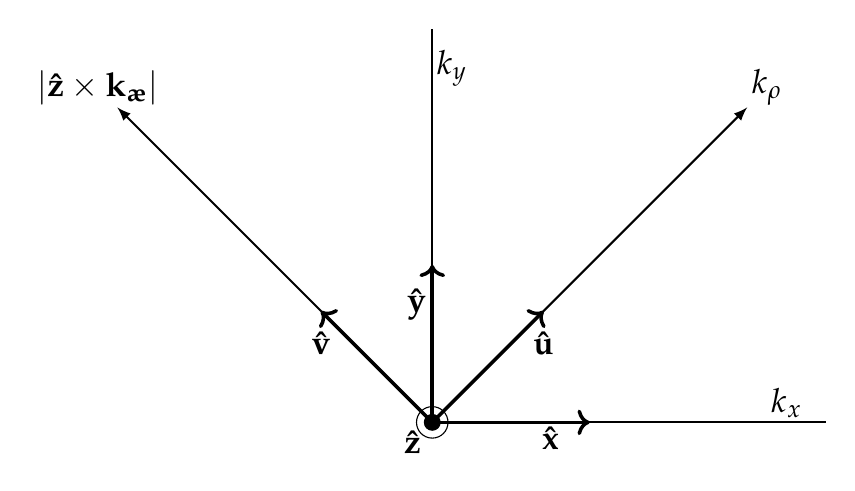
\begin{tikzpicture}
    % Draw coordinate system
    \draw [color=black, fill=black] (0, 0) circle (0.1);
    \draw [color=black, fill=none] (0, 0) circle (0.2);
    % x-axis
    \draw [line width=0.25mm] (0, 0) -- (5, 0);
    % y-axis
    \draw [line width=0.25mm] (0, 0) -- (0, 5);
    % x-axis label
    \node at (4.5, 0.25) {$k_x$};
    % y-axis label
    \node at (0.25, 4.5) {$k_y$};

    % unit x-axis
    \draw [line width=0.45mm,->] (0, 0) -- (2, 0);
    % unit y-axis
    \draw [line width=0.45mm,->] (0, 0) -- (0, 2);
    % origin label
    \node at (-0.25, -0.25) {$\mathbf{\hat z}$};
    % Unit x-axis label
    \node at (1.5, -0.2) {$\mathbf{\hat x}$};
    % Unit y-axis label
    \node at (-0.2, 1.5) {$\mathbf{\hat y}$};

    % Rotated Coordinates
    % k_p
    \draw [line width=0.25mm,arrows={-latex}] (0, 0) -- (4, 4);
    % k_p-axis label
    \node at (4.25, 4.25) {$k_{\rho}$};
    % unit u-axis
    \draw [line width=0.45mm,->] (0, 0) -- (1.412, 1.412);
    % unit v-axis
    \draw [line width=0.45mm,->] (0, 0) -- (-1.412, 1.412);
    % Unit u-axis label
    \node at (1.412, 1) {$\mathbf{\hat u}$};
    % k_p perpendicular
    \draw [line width=0.25mm,arrows={-latex}] (0, 0) -- (-4, 4);
    % Unit v-axis label
    \node at (-1.412, 1) {$\mathbf{\hat v}$};
    % k_p-axis perpendicular label
    \node at (-4.25, 4.25) {$|\mathbf{\hat z} \times \mathbf{k_{\rho}}|$};
  \end{tikzpicture}
\end{document}

  \caption{Coordinate System transformation in the spectral domain}
  \label{fig:SpCS}
\end{figure}

%
Using the results of \eqref{eq:EHVI} in \eqref{eq:Et} and noting that $\v{\^u} = \v{k_{\p}}/k_{\p}$, we get,
%
\begin{equation}
  \dv{\left(\v{\^u} \, V^{TM} + \v{\^v} \,V^{TE} \right)}{z} = \frac{1}{\j \O \E}\left( k^2 - \v{k_{\p}} \,\v{k_{\p}} \,\cdot \right) (\v{\^u}\, I^{TM} + \v{\^v} \, I^{TE}) + \v{\^u} \, \frac{k_{\p}}{\O \E} \ti{J}_z
  \label{eq:Vinuv}
\end{equation}
%
By separating the $\v{\^u}$ and $\v{\^v}$ components, we obtain the TM and TE equivalent voltage equations respectively,
%
\begin{subequations}
  \begin{align}
    \dv{V^{TM}}{z} ={}&
    \frac{1}{\j \O \E}\left( k^2 - k_{\p}^2 \right)I^{TM} + \frac{k_{\p}}{\O \E} \ti{J}_z,
    \label{eq:V_TM}\\
    \dv{V^{TE}}{z} ={}&
    \frac{k^2}{\j \O \E} I^{TE}.
    \label{eq:V_TE}
  \end{align}
  \label{eq:TL_Vs}%
\end{subequations}
%
Similarly, from \eqref{eq:EHVI} and \eqref{eq:Ht}, the equivalent current equations can be written as:
%
\begin{subequations}
  \begin{align}
    \dv{I^{TM}}{z} ={}&
    \frac{k^2}{\j \O \u} V^{TM} - \ti{J}_u,
    \label{eq:I_TM}\\
    \dv{I^{TE}}{z} ={}&
    \frac{-1}{\j \O \u}\left( k^2 - k_{\p}^2 \right)V^{TE} + \ti{J}_v.
    \label{eq:I_TE}
  \end{align}
  \label{eq:TL_Is}%
\end{subequations}
%
Equations \eqref{eq:TL_Vs}-\eqref{eq:TL_Is} can be conveniently written in a compact form as a set of Telegrapher's equations \cite[p. 1166]{michalski2005}:
%
\begin{subequations}
  \begin{align}
    \dv{V^{\alpha}}{z} ={}& -\j k_z Z^{\alpha}I^{\alpha} + v^{\alpha}
    \label{eq:TL_V}\\
    \dv{I^{\alpha}}{z} ={}& -\j k_z Y^{\alpha}V^{\alpha} + i^{\alpha}
    \label{eq:TL_I}
  \end{align}
  \label{eq:TLE}%
\end{subequations}
%
where the propagation constant in the transverse direction is,
%
\begin{equation}
  k_z = \pm \sqrt{k^2 - k_{\p}^2}
  \label{eq:k_z}
\end{equation}
%
and the modal impedances are,
%
\begin{subequations}
  \begin{align}
    Z^{TM} = \frac{1}{Y^{TM}} = \frac{k_z}{\O \E},
    \label{eq:z_tm}\\
    Z^{TE} = \frac{1}{Y^{TE}} = \frac{\O \u}{k_z}.
    \label{eq:z_te}
  \end{align}
  \label{eq:Z}%
\end{subequations}
%
Assuming only electric sources existing in space, the corresponding TL sources, $v^{\alpha}$ and $i^{\alpha}$, where $\alpha$ is either TE or TM, are illustrated in \ref{fig:J_sources}. A horizontally oriented (x-directed) electric dipole is represented by a current source in an equivalent TM transmission line network. Likewise, the equivalent configuration of a vertical (y-directed) electric dipole is a TE network with a current source. A z-directed dipole corresponds to voltage source in a TM transmission line. For an arbitrarily directed source, the equivalent TL model consists of a superposition of the three representations.
%
\begin{figure}[h]
  \centering
  \subfloat[]{\centering
  \includegraphics[width=.55\textwidth]{figures/jx.tikz}
  \label{fig:jx_source}}  \newline
  \subfloat[]{ \centering
  \includegraphics[width=.55\textwidth]{figures/jy.tikz}
  \label{fig:jy_source}}  \newline \centering
  \subfloat[]{\centering
  \includegraphics[width=.55\textwidth]{figures/jz.tikz}
  \label{fig:jz_source}} \newline
  \caption{Electric Source representation in a transmission line network}
  \label{fig:J_sources}
\end{figure}
%%%
%%%
%%%
%%%
\subsection{Equivalent TL network of semiconductor heterostructures}
%
In modern semiconductor devices such as a field-effect transistor, multiple layers of materials with slightly different dielectric properties and band-gap energies are epitaxially grown over each other. Of particular interest are the group III-V materials in which extra-ordinary electromagnetic interfacial phenomena is observed, mainly due to formation of a two-dimensional electron gas (2DEG) at the interface. To develop an understanding of the unusual properties of what are commonly called semiconductor heterostructures, we construct an equivalent transmission model of the layered structure using the theory discussed in the previous section.

An illustration of a multilayer setup with a heterostructure near the top of the transistor substrate, through which modern devices like the high electron mobility transistor operate, is shown in Fig. \ref{fig:TL_equivalent}a. Although a number of other material layers lie underneath the heterostructure that are essential to the fabrication process, primarily to strengthen the epitaxial structure, only the top layers are conducive to an electric field. Moreover, since the widths of the layers in the heterostructure are much smaller than the rest of the layers in the substrate stack, we assume that the heterostructure is unbounded from the bottom.

The 2DEG which is only a few atoms wide in thickness, is a highly conductive region with an abundance of free electrons, which can be expresses in terms of a surface conductivity \cite{Burke2000},
%
\begin{equation}
  \sigma_s = \frac{N_s e^2 \tau}{m^{\ast}}\frac{1}{1 + \j \O \tau},
  \label{eq:sigma_s}
\end{equation}
%
where $N_s$ is the free electron concentration at the interface, $e$ is the electron charge, $m^{\ast}$ is the effective electron mass in the heterostructure, $\tau$ is the scattering time of electrons, and $\O$ is the angular frequency. For a wave propagating along the interface, the electron scattering time which is highly temperature dependent, determines the attenuation factor. At room temperature, the thermal vibrations of electrons result in a very small value of $\tau$ which is of the order of femtoseconds (\SI{1e-15}{\s}), leading to a high-loss scenario. On the other hand, when the heterostructure is cooled to temperatures close to the boiling point of helium (\SI[round-precision=2]{4.2}{\kelvin}), thermal vibrations are effectively removed and the losses are consequently minimized.

In a transmission line analogue, the equivalent representation of a conductive sheet such as a 2DEG is a shunt admittance as shown in Fig. \ref{fig:TL_equivalent}b. In a high electron mobility transistor, when a voltage bias is applied across the source and drain terminals, a current starts to flow laterally, inside the 2DEG. Such a current source, configured horizontally corresponds to Fig. \ref{fig:jx_source}, which translates to a TM-mode transmission line excited by a current source. The presence of a gate terminal above or below the interface allows the electron concentration to be modified by the gate voltage. Therefore, instead of an independent current source in the equivalent transmission line network, a voltage-controlled current source is placed as indicated in Fig. \ref{fig:TL_equivalent}.
%
\begin{figure}[t!]
  \centering
  \def\svgwidth{\linewidth}
  \input{figures/multilayers.pdf_tex}
  \caption{(a) Multilayer structure typically found in a high electron mobility transistor, (b) Equivalent transmission line network}
  \label{fig:TL_equivalent}
\end{figure}
%

We determine the dispersion relation in a 2DEG region which lies embedded in a semiconductor stack. As stated earlier, the active state of the transistor in which a current flows through the 2DEG corresponds to a TM-mode transmission line network. It must also be mentioned that a similar TL analogue can be obtained if the physical structure is excited by a TM-polarized plane wave. The dispersion relation can be written using the transverse resonance method that requires the total admittance as seen from the 2DEG (at z = 0) to be zero \cite{Gomez-Diaz2012},
%
\begin{equation}
  Y^{\uparrow}(z_0) + Y^{\downarrow}(z_0) + Y_{\sigma} = 0.
  \label{eq:dispersion}
\end{equation}
%
Here, $Y^{\uparrow}(z_0)$ and $Y^{\downarrow}(z_0)$ are the up- and down-looking TL admittances from the 2DEG located at $z = 0$ and $Y_{\sigma} = \sigma_s$ from \eqref{eq:sigma_s}.

A nontrivial solution of \eqref{eq:dispersion} in terms of the propagation constant $k_{\p}$ yields the surface wave modes of the structure in the complex k-plane.
%%%%%%%%%%
%%%%%%%%%%
%%%%%%%%%%
%%%%%%%%%%
%%%%%%%%%%
\section{Surface waves extraction technique}
%
We seek to solve \eqref{eq:def} in the complex z-plane to obtain the zeros, $z_k$ in a given search region $\mathbb{C}$. For a multilayer problem such as the one shown in Fig. \ref{fig:TL_equivalent}a, $f$ represents the dispersion relation \eqref{eq:dispersion} which, in fact is the denominator of the  transmission line Green function (TLGF). From hereon, $k_{\p}$ is replaced by $z$ for notational simplicity. Depending on the location of the zeros of the function $f$ in the complex plane, $z_k$'s can be termed as the surface wave modes of the multilayer or synonymously, poles of the TLGF.
%
\begin{equation}
  f(k_{\p}) = 0
  \label{eq:def}
\end{equation}
%
Although the problem at first, may appear to be a relatively simple root-search in which readily available and popular iterative algorithms like the Newton or Halley's method can be applied, complication arises due to the presence of complex-valued roots. Furthermore, the convergence of the aforementioned methods is highly subject to an initial guess that must lie close to the actual root. As an example, basins of attraction, which illustrate the convergence rate of an initial guess, are shown in Fig. \ref{fig:basins} for Newton's and Halley's methods which are two of the most popular iterative root-finding methods. In Fig. \ref{fig:basins}, the actual roots of a polynmial, $z^{10}-1$ are depicted by circle marks. The regions are color-coded for each root where a large area of a particular color indicates that if the initial guess is located in that region, convergence to the respective root will be achieved quickly. On the other hand, if the initial guess lies in the fractal region, the convergence is very slow. Another observation through which Newton and Halley's methods can be compared is that the basins of attraction of Newton's method,
shown in Fig. \ref{fig:newton} have a denser fractal region due to its quadratic complexity of convergence. On the contrary, the Halley's method, which is cubic, the fractals are comparatively sparse as shown in Fig. \ref{fig:halley}.

For a dispersion relation \eqref{eq:dispersion}, which is defined by a transcendental equation, presence of singularities, particularly in the vicinity of an actual solution may leave an iterative method completely divergent or yet churn out a bogus and unreliable answer.

Argument principle method (APM) is a robust, complex root-finding algorithm in which convergence is guaranteed within a specified region without supplying any initial guess \cite{Delves1967c,Carpentier1982c,Botten1983,Kravanja2000c,Dellnitz2002c,Gillan2006c,Chen2017}. It requires the function to be analytic in the specified search region. A pictorial representation of this technique is shown in Fig. \ref{fig:zplane} where the roots inside a specified region $\Gamma$ in the complex plane are computed by approximating the given function with a polynomial. In case, the number of zeros inside $\Gamma$ exceed a pre-allocated value $N_r$, the search region is subdivided into smaller regions. Moreover, the function $f$ must be non-zero at the boundary of $\Gamma$. The following sections briefly describe each step of the method.
%
\begin{figure}[t!]
  \centering
  \subfloat[]{\includegraphics[height = 2.7in]{basin_fig.tikz}
  \label{fig:newton}} \hfil
  \subfloat[]{\includegraphics[height = 2.7in]{hbasin_fig.tikz}
  \label{fig:halley}}
  \caption{Complex plane basin of attraction while solving $z^{10} - 1 =0$ using: (a) Newton's method (c) Halley's method}
  \label{fig:basins}
\end{figure}
%
%%
\begin{figure}[t!]
  \centering
  \def\svgwidth{.5\linewidth}
  \input{figures/zplane.pdf_tex}
  \caption{Illustration of the root-finding routine in the presence of branch point singularities. Only proper modes are sought within a rectangular controur $\Gamma$}
  \label{fig:zplane}
\end{figure}
%%
%%
%%
\subsection{Counting the zeros}
%
To develop an efficient method of locating the zeros, we assume that the function $f$ is analytic, which implies that it is differentiable and free from any singularities. It is also required that $f$ is non-zero at the boundary, $\Gamma$ of the region $\mathbb{C}$. The search region is set as rectangular, mainly because of ease in programming it. The number of zeros, $N$ inside a region with a boundary $\Gamma$ can be found using the Cauchy's integral theorem \cite[pg. 71]{Krantz1999,Delves1967c},
%
\begin{equation}
  N = \frac{1}{2 \pi \j} \oint \limits_{\Gamma} \frac{f'(z)}{f(z)} \diff{z}
  \label{eq:cauchyth}
\end{equation}
%
where the integrand is a logarithmic derivative of the function. The analytical derivative of functions such as found in dispersion relations like \eqref{eq:dispersion} are seldom readily-available and it is generally cumbersome to compute. In this chapter, we use approximate the derivative by a finite difference formula,
%
\begin{equation}
  f'(z) = \frac{f(z + h) - f(z - h)}{2 h},
  \label{eq:FD}
\end{equation}
%
where $h \sim \sqrt{\epsilon_m}$ and $\epsilon_m = \SI{2.2204e-16}{}$ is the double-precison machine accuracy \cite[pg. 230]{press2007numerical}.

In addition to \eqref{eq:cauchyth}, a derivative-free form of the argument principle \cite{Carpentier1982c,Gillan2006c}, which may be preferred in certain cases is,
%
\begin{equation}
 N = \frac{1}{2 \pi} \oint \limits_{\Gamma} \diff {\{ \arg f(k_{\p})\}},
 \label{eq:numzeros}
\end{equation}
%
The value of both the integrals, i.e., \eqref{eq:cauchyth} and \eqref{eq:numzeros} is an integer which means that whenever a zero is encountered that appears as a pole in the integrand, the resulting integral is incremented by a factor of $2 \pi$ by Caucy's residue theorem. The contour integration in \eqref{eq:cauchyth} and \eqref{eq:numzeros} is computed in a counter-clockwise manner, using an adaptive Gauss-Konrod quadrature ({MATLAB}'s \emph{quadgk} routine) \cite{Shampine2008}. The contour can be conveniently set up using the `waypoints' parameter of the routine.
%%
%%
%%
%%
\subsection{Locating the zeros}
%
In this chapter, we use the derivative-free approach \eqref{eq:numzeros} to compute the number of zeros and further on. After predicting the number of zeros, the function $f$ is then approximated by an associated \emph{formal orthogonal polynomial} (FOP), $\mathcal P$ of degree $N$, equal to the number of zeros. A necessary condition during approximation is that $\mathcal P$ must have the same roots, $z_k$ where $k = 1,2,...,N$ as $f$. Furthermore, as stated earlier $N$ must be less than $N_r$ to avoid a too-high order polynomial for which the root-finding procedure would be very slow.

The polynomial $\mathcal P$ can be represented in a Lagrange form:
%
\begin{equation}
  \begin{split}
    \mathcal{P}_N(z) ={}& \prod \limits_{k = 1}^N \left(z - z_k \right) \\
    ={}& z^N + \sigma_{N-1} \, z^{N-1} + \dots + \sigma_{1} \, z + \sigma_0.
  \end{split}
  \label{eq:poly}%
\end{equation}
%
To find the coefficients, $\sigma_k$ we first define a symmetric bilinear operator similar to a dot product \cite{Kravanja1999,Gillan2006c},
%
\begin{equation}
  \left \langle \phi, \psi \right \rangle = \frac{1}{2 \pi \j} \oint \limits_{\Gamma} \phi(z) \, \psi(z) \frac{1}{f(z)} \diff{z}
  \label{eq:blinear}
\end{equation}
%
where $\phi$ and $\psi$ are polynomials of $z$. Next, we consider a set of integrals that are termed as the \emph{Newton moments},
%
\begin{equation}
  s_p = \left \langle 1, z^p \right \rangle \frac{1}{2 \pi \j} \oint \limits_{\Gamma} z^p \frac{1}{f(z)} \diff{z}.
  \label{eq:s_p}
\end{equation}
%
which are then used as elements to construct Hankel matrices of size $N$,
%
\begin{equation}
  \mathbf H =
  \begin{bmatrix}
    s_1 & s_2 & \cdots & s_k \\
    s_2 & s_3 & \cdots & s_{k+1} \\
    \vdots & \vdots & \ddots & \vdots \\
    s_k & s_{k+1} & \cdots & s_{2k} \\
  \end{bmatrix}
  \label{eq:Hmat}
\end{equation}
%
and
%
\begin{equation}
  \mathbf H^< =
  \begin{bmatrix}
    s_0 & s_1 & \cdots & s_{k-1} \\
    s_1 & s_2 & \cdots & s_{k} \\
    \vdots & \vdots & \ddots & \vdots \\
    s_{k-1} & s_{k} & \cdots & s_{2k-2} \\
  \end{bmatrix},
  \label{eq:Hmat<}
\end{equation}
%
in which the secondary diagonal terms are the same.

The polynomial $\mathcal P$ in \eqref{eq:poly} is orthogonalized by enforcing the condition,
%
\begin{equation}
  \left \langle z^k, \mathcal {P}_N(z) \right \rangle, \quad \text{where} \, k = 0,1,\dots,N-1.
  \label{eq:orthogonalzie}
\end{equation}
%
Because the operator $\left \langle \cdot, \cdot \right \rangle$ defined in \eqref{eq:blinear} is not a dot product in true sense, that is why the term \emph{formal} is included in the definition of the polynomial \cite{Kravanja1999}.
%

The polynomial in \eqref{eq:poly} can also be equivalently represented by a \emph{companion} matrix, $A$ as,
%
\begin{equation}
  \mathbf A =
  \begin{bmatrix}
    0 & 1 & 0 & \cdots & 0 \\
    0 & 0 & 1 & \cdots & 0 \\
    \vdots & \vdots & \ddots & \vdots \\
    0 & 0 & 0 & \cdots & 1 \\
    -\sigma_0 & -\sigma_1 & -\sigma_1 & \cdots & \sigma_{N-1} \\
  \end{bmatrix},
  \label{eq:A}
\end{equation}
%
and $\mathcal P_n(z)$ can be obtained by setting its characteristic equation \cite{Gentle1998},
%
\begin{equation}
  \det( A - \sigma_k I) = P(z),
  \label{eq:xticeq}
\end{equation}
%
where the eigenvalues are given by $\sigma_k$ for the eigenvector $z$. The eigenvalue value problem of \eqref{eq:xticeq} can not be solved since the coefficients $\sigma_k$'s, where $k = 0, 1, 2, \dots, N-1 $, are not known yet. However, we can express $\sigma_k$'s in terms of the \emph{Newton moments}, $s_k$'s through the \emph{Newton identities}:
%
\begin{equation}
  \begin{aligned}
    & s_1 + \sigma_1 = 0 \\
    &  s_2 + s_1 \sigma_1 + 2 \sigma_2 = 0 \\
    &  {\vdots}\\
    &  s_N + s_{N-1} \sigma_{1} + ... + s_1 \sigma_{N-1} + s_0 \sigma_N = 0.
    \label{eq:newtid}
  \end{aligned}
\end{equation}
%
where we note that $s_0 = N$. We therefore, construct an equivalent eignevalue problem using \eqref{eq:Hmat}, \eqref{eq:Hmat<} and \eqref{eq:newtid} \cite{Gillan2006c},
%
\begin{equation}
  \left( \mathbf H - \lambda_k \mathbf H^< \right) \mathbf z = 0
  \label{eq:evp}
\end{equation}
%
where the column vector $\mathbf{z}$ is an eigenvector and $\lambda_k$'s are the eigenvalues of the matrix pencil $(\mathbf H - \mathbf H^< )$, which correspond to the roots of $\mathcal P_n(z)$. In {MATLAB}, the routine \emph{eig} is used to solve \eqref{eq:evp}.
%%
%%
%%
%%
\subsection{Refining the roots}
%
% Approximating a function in a given contour with many zeros requires a higher-order polynomial that introduces computational problems. In addition, the integrals of the moments in \eqref{eq:sk} need to be evaluated with a higher-accuracy and the mapping between $s_k$ and $\alpha_k$ \eqref{eq:newtid} rseults in an ill-conditioned system. To overcome such pitfalls, a limit is enforced on the number of zeros in a given region. If the number of zeros exceeds a predetermined value $M$, the size of the search region is subdivided \cite{Delves1967c}.
The accuracy of the roots obtained from the eigenvalues, $\lambda_k$ of \eqref{eq:evp} is not always high. However, $\lambda_k$'s is an excellent initial guess for any iterative root-search routine from the class of Householder's methods. We choose the \emph{Newton} method \cite{press2007numerical} having quadratic convergence and the iteration formula:
%
\begin{equation}
  x_{n+1} = x_n - \frac {f(x_n)}{f'(x_n)}
  \label{eq:newton}
\end{equation}
%
with $f'(x)$ is the first order derivative approximated by a finite difference formula \eqref{eq:FD}. In general, the roots $z_k$'s are complex, therefore, the iteration \eqref{eq:newton} needs to be performed on both the real and imaginary parts simultaneously.
%%
%%
%%
%%
\subsection{Avoiding singularities}
%
As mentioned earlier, the argument principle method requires the function to be analytic without any singularities. In this chapter, we explicitly deal with the dispersion relation \eqref{eq:dispersion} which is the denominator expression of the transmission line Green function. Therefore, branch point singularities only occur due to the presence of multivalued square roots that appear in the definition of the propagation constant, $k_{z,i}$ \eqref{eq:k_z} with $i =1,\dots, N$ and, $N$ being the number of layers. The branch points exist provided the top and bottom layers are unbounded. The dispersion relation shows an even dependence on $k_{zi}$ due to the layers that are bounded, hence they do not  contribute any branch points \cite[Section~5.3a]{felsen1994,Felsen1994}. In the worst case where the top and bottom layers are open and different from each other, two branch points exist in the complex plane that must be either removed or avoided in order to make the function analytic in the search region. Additionally, branch cuts emerge out of the branch points and there must not be any intersection with the contour of the search region.

In order to remove the branch point singularities, the complex z-plane is generally mapped to another plane $\zeta$, by a transformation that unfolds the Riemann surface. For example, a trigonometric transformation such as \cite{Michalski2006,Polimeridis_2007},
%
\begin{equation}
  \begin{split}
    z &\mapsto \zeta \\
    \zeta &= \cos (z),
  \end{split}
  \label{eq:mapping}%
\end{equation}
%
removes the branch point due to the multivalued propagation constant, $k_{zi}$, where $i = 1,N$ and makes the dispersion relation \eqref{eq:dispersion} analytic in the $\zeta$-plane.
%
%

In this chapter, our goal is to find the surface waves from the dispersion relation. We only seek the \emph{proper modes}, which are the roots of \eqref{eq:dispersion} that lie to the right of the branch point corresponding to $\max(k_{z1},k_{zN})$. In order to satisfy the Sommerfeld radiation condition which requires all fields to decay to zero at infinity, the proper sheet of the Riemann surface of the square-root function needs to be selected. This is accomplished by enforcing that the imaginary part of $k_{zi}$ that contributes a branch point, is negative everywhere.
%
\begin{equation}
  \Im (k_{zi}) < 0
  \label{eq:proper}
\end{equation}
%
%%%%%%%%%%%%%%%
%%%%%%%%%%%%%%%
%%%%%%%%%%%%%%%
\section{Results}
%
\subsection{MIM waveguide}
%
%
We first compute the modes of a metal-insulator-metal (MIM) waveguide described in \cite{Kocabas2009}. An air-filled region of thickness $d = \lambda/4$, where $\lambda = \SI{1550}{\nm}$ is sandwiched between two metal layers having permittivity $\E_m$. We first consider a lossless case in which $\E_m$ has a value of $-143.4967$, because of which the complex plane is essentially free from any branch-point singularities. For a TM case the dispersion relation is written as:
%
\begin{equation}
  D =  1 - \left(\frac{Z_m - Z_2}{Z_m + Z_2}\right)^2 \x \e^{(-2\j  k_{z2} d)},
  \label{eq:mim}
\end{equation}
%
where $Z_m = k_{zm}/(\O \E_m \E_0)$ and $Z_2 = k_{z2}/{\O \E_0}$ are the modal impedances of the metal and air-filled layers respectively. The TM modes of \eqref{eq:mim} normalized to the free-space propagation constant are shown in Fig. \ref{fig:mim_lossless}. The values of the roots obtained are then compared with the solutions discussed in \cite{Kocabas2009}, in which only the even modes were computed. However, as listed in Table. \ref{tab:kocabas_lossless}, we compute first nine even and odd modes.
%
\begin{table}[!htbp]
\begin{center}
 \begin{tabular}{||c |c |c||}
 \hline
 Mode & This method \eqref{eq:mim} & Kocaba{\c{s}} et. al. \cite{Kocabas2009} \\ [0.5ex]
 \hline\hline
 $\text{TM}_0$ & \num{12.020580892546883 - j 0.004431747015808} & \num{12.02521374394057} \\
 $\text{TM}_1$ & \num{11.853246184016845 - j 0.008865820349836} & \num{} \\
 $\text{TM}_2$ & \num{11.336574483861385 - j 0.008867713656375} & \num{11.34454132059978} \\
 $\text{TM}_3$ & \num{10.418519825598594 - j 0.008867285000744} & \num{} \\
 $\text{TM}_4$ & \num{8.976849574973341 - j 0.008867077386298} & \num{8.98087712606770} \\
 $\text{TM}_5$ & \num{6.680787568724169 - j 0.008866971189904} & \num{} \\
 $\text{TM}_6$ & \num{0.832396034296521 - j 0.008866910825003} & \num{0.7136870643968289} \\
 $\text{TM}_7$ & \num{0.000000000000000 - j 7.149095944697479} & \num{} \\
 $\text{TM}_8$ & \num{0.000000000000000 - j 10.534126133587652} & \num{0.00887301858491 - j 10.55951095636977} \\
 \hline
 \end{tabular}
  \end{center}
 \caption{TM modes of a lossless MIM waveguide}
 \label{tab:kocabas_lossless}
\end{table}
%

Next, we consider the lossy case where the permittivity of metal layers is $\E_m = \num{-143.4967 + j 9.5173}$ and the compared results are shown in Fig. \ref{fig:mim_lossless} and listed in Table. \ref{tab:kocabas_lossy}.
%
\begin{table}[!htbp]
\begin{center}
 \begin{tabular}{||c |c |c||}
 \hline
 Mode & This method \eqref{eq:mim} & Kocaba{\c{s}} et. al. \cite{Kocabas2009} \\ [0.5ex]
 \hline\hline
 $\text{TM}_0$ & \num{12.027529836826002 - j 0.400073290979892} & \num{12.03170325421919 - j 0.39535643587620} \\
 $\text{TM}_1$ & \num{11.860919992851576 - j 0.410048132657156} & \num{} \\
 $\text{TM}_2$ & \num{11.345243844591128 - 0.428274354267573i} & \num{11.35226216175467 - i0.41892103144838} \\
 $\text{TM}_3$ & \num{10.429478086718880 - 0.465101072534315i} & \num{} \\
 $\text{TM}_4$ & \num{8.993535082138010 - 0.537950132567878i} & \num{8.99644754875734 - i0.52888321538511} \\
 $\text{TM}_5$ & \num{6.719731462664607 - 0.716992164959356i} & \num{} \\
 $\text{TM}_6$ & \num{2.266946388295501 - 2.107982239061171i} & \num{2.247924588647662 - i2.124681976891650} \\
 $\text{TM}_7$ & \num{0.661173227981735 - 7.188483710355326i} & \num{} \\
 $\text{TM}_8$ & \num{0.450360863091437 - 10.543804519180030i} & \num{0.45907739584359 - i 10.56851955358188} \\
 \hline
 \end{tabular}
  \end{center}
 \caption{TM modes of a lossy MIM waveguide}
 \label{tab:kocabas_lossy}
\end{table}
%
\begin{figure}[!htbp]
  \subfloat[]{\includegraphics[height=2.5in]{kocabas_lossless.tikz}
      \label{fig:mim_lossless}}
      \hfil
      \subfloat[]{\includegraphics[height=2.5in]{kocabas_lossy.tikz}
          \label{fig:mim_lossy}}
  \caption{TM modes of a MIM waveguide (a) Lossless case, $(\E_m = \num{-143.4967})$ (b) Lossy case, $(\E_m = \num{-143.4967 + j 9.5173})$}
  \label{fig:mim}
\end{figure}
%
\subsection{Embedded conductive sheets}
%
%
Here we plot the dispersion curves of a 2DEG which is considered as a thin sheet embedded in a semiconductor heterostructure. We look at three types of structures,
%
\begin{enumerate}
  \item Gated 2DEG
  \item Ungated 2DEG
  \item Backgated 2DEG,
\end{enumerate}
%
that are classified, based on the presence of a perfectly conducting covering layer either at the top or bottom. The three types are shown in Fig. \ref{fig:2deg_structure_types}.
%
\begin{figure}[!htbp]
  \subfloat[]{\def\svgwidth{.3\linewidth}
  \input{figures/gated.pdf_tex}
  \label{fig:gated}} \hfil
  \subfloat[]{\def\svgwidth{.3\linewidth}
  Generation of Plasma waves

Talk about ungated plasma waves
dispersion relation
dyakanov-shur instability
resonance
terahertz
conductivity
mobility
dielectric function approximated


For the ungated 2DEG, the dispersion relation is given by:
\begin{equation}
  \O = \sqrt{Ne^2 /m_s}
  \label{eq:ungated_disp}
\end{equation}

The plasma frequency for an ungated region is an order of magnitude higher than the gated region of the transistor. Moreover, the Q-factor of the resonance is also higher. This paves the way for devices operating in the range of 20-30 THz. Some of the molecules found in biological sciences fluoresce in this region. Therefore, plasma oscillations that are resonant can be used to excite these molecules.

The generation of plasma waves in the gated region has been thoroughly studied owing to their analogy with the shallow water waves found in hydrodynamics. A similar treatment of plasma waves in the ungated region are analagous to deep water waves {\cite Shur ungated}.

When the plasma waves come across appropriate boundary conditions in the form of an ac open short source and and dc short drain terminal, they tend to reflect and form a standing wave in the 2DEG. Further excitement of these plasma waves lead to their instability. For an ungated region, due to the absence of grating structure in the form of the gate terminal, the plasma waves tend to not radiate as efficiently due to the momentum mismatch (large difference of wavenumber) between the plasma waves and free-space. However, due to the very thin nature of the superstatet spacer layer on the 2DEG, partially decayed plasma waves exist at the top face of the structure which can be used to excite the sample.

In order to obtain a strong standing wave pattern, the device should be operated near the plasma frequency so that the dielectric function of the 2DEG region is vanishingly small. Furthermore, the real part of the conductivity is much smaller than its imaginary part. The conductivity is given by:

\begin{equation}
    \sigma_s(\O) = \frac{N_s e^2}{m_{\ast}} \tau \frac{1}{1 + j \O \tau}
    \label{eq:conductivity}
\end{equation}

The quantity $\tau$ is the mean scattering time of the electrons in the 2DEG which is expressed in terms of the electron mobility:

\begin{equation}
  \tau = \frac{\u m_{\ast}}{e}
  \label{eq:tau}
\end{equation}

In order to obtain the desired properties for conductivity and dielectric function discussed above, the mobility should be as high as possible. Unfortunately, it is highly temperature dependent and reduces exponentially with increase in temperature by the following relation:

\begin{equation}
  \u \prop \frac{1}{T^{3/2}}
  \label{eq:uT}
\end{equation}

Thus the device must be cooled to cryogenic temperatures. Moreoever if the product $\O \tau >> 1$, the oscillation in the 2DEG are undamped.

For thin structures, the sheet conductivity can be converted into an approximate volumetric form by the multplying with the thickness of the 2DEG layer. The resulting dielectric function is then written as:

\begin{equation}
  \E(\O) = \E_0 \E_r + j\frac{\sigma_s(\O)}{\O t \E_0}
\end{equation}

Write about the dielectric function
Dispersion relation
Simulation

GaN/AlGaN heterostructure

Structure details

We consider a Gallium Nitride / Aluminum Gallium Nitride (GaN / AlGaN) semiconductor heterostructure whose material properties are taken from [\cite popov paper, nitronex template]. The length of structure is taken as $.1 \mu m$. The layer thickness of the 2DEG region is taken as $5 nm$ and the superstrate layer is $20 nm$ thick. When a TM polarized plane wave having electric field components in the plane of the structure is incident on the structure, the dispsersion relation can be derived by expressing fields in each region of the structure. Although the structure is finite in length, for the sake of simplicity, it is assumed here that the structure has infinte lateral dimensions. The dispersion relation can be written as:

\begin{equation}
  disp equation expression
  \label{eq: dispersion}
\end{equation}

It should be pointed out only in the case of a TM polarized do we get real solutions of propagation constant from the dispersion relation. For TE case, the real solutions are obtained only when an anisotropic conductivity of the 2DEG layer is assumed.

Simulation details:

The structure under observation is simulated in COMSOL using the RF module where a TM polarized plane wave is used to excite the structure. Furthermore, in order to model the charges in the 2DEG region, a surface current density is inserted expressed in terms of the complex surface conductivity and the electric field by:

\begin{equation}
  J_s (x) = \sigma_s(\O) E_x
  \label{eq:Js}
\end{equation}

This current is due to the tangential boundary conditions applied on the magnetic field. The 2DEG and spacer layers are terminated in a PEC to model the source and drain terminals of the transistor. For absorbing boundary conditions, Scattering boundary condition is applied on the outer perimeter of the structure. Figure shows the standing wave pattern obtained on the face of the structure. The structure is sumulated at $25$ THz where the conductivity is $6.9 \times 10^{-8} + j 7.15 \times 10^{-5}$ [S/m]  and the corresponding dielectric constant for a layer of thickness $5$ nm is $-.878 + j 5.3 \times 10^{-3}$. The free charge density at the GaN / AlGaN interface is typically $7.5 \times 10 ^{12} \mathrm{cm}^{-2}$ with the mobility of $10^{6} \mathrm{C/cm^{-2}/s}$ at temperature of $3$ K. The dielectric constants of GaN and AlGaN layers are 9.7 and 9.4 repsectively where the mole fraction of the AlGan is taken as $x = .54$.

Shifting of the Pattern

One of the key requirements of Structured Illuminatiom Microscopy is that the standing wave pattern be shifted laterally. This is achieved by shining a TM polarized plane wave beam on the structure and controlling the magnitudes of the components of the electric field. For the configuration with the boundary conditions discussed above, the electric field component along the 2DEG will be cosine function and the normal component is a sine function.

  \label{fig:ungated}} \hfil
  \subfloat[]{\def\svgwidth{.3\linewidth}
  \input{figures/backgated.pdf_tex}
  \label{fig:backgated}} \hfil
  \caption{2DEG embedded in a semiconductor heterostructure at $z=0$ (a) Gated  (b) Ungated (c) Backgated}
  \label{fig:2deg_structure_types}
\end{figure}
%

We consider GaN/AlGaN (gallium nitride / aluminum gallium nitride)  heterostructure with Al mole-fraction of $x = \num[round-precision=1]{0.2}$. With respect to Fig. \ref{fig:2deg_structure_types}, Layer 1 is composed of GaN which is the substrate, considered open in the gated and ungated cases, while it has a thickness of $d = \SI{50}{\nm}$ in the backgated case. AlGaN forms the layer marked 2, and in all the three cases, a thickness, $h = \SI{20}{\nm}$ is assumed. The permittivity of both the layers is $\E_r = 9.5$ owing to the small aluminum mole fraction \cite{Muravjov2010}. The electron concentration of the 2DEG region is $N_s = \SI{5e13}{\cm^{-2}}$ and scattering time $\tau$ of \SI{114}{\ps} corresponding to a temperature of \SI{3}{\kelvin} is assumed. The surface conductivity is then computed using \eqref{eq:sigma_s}. When solving for the dispersion relation \eqref{eq:dispersion}, we use the respective expressions listed in Table. \ref{tab:equations} for each case.
%
\begin{table}[!htbp]
\begin{center}
 \begin{tabular}{||c |c |c||}
 \hline
 Gated & Backgated  & Ungated \\ [0.5ex]
 \hline\hline
 $Y^{\uparrow} = - Y_{2} \coth (k_{z2} h)$ & $Y^{\uparrow} = Y_{2} \frac{1 - \Gamma^{\uparrow}}{1 + \Gamma^{\uparrow}}$ & $Y^{\uparrow} = Y_{2} \frac{1 - \Gamma^{\uparrow}}{1 + \Gamma^{\uparrow}}$ \\  & & \\ [2ex]
\num{} & $\Gamma^{\uparrow} = \frac{Y_2 - Y_1}{Y_2 + Y_1} \e^{-2\j k_{z2}\, h}$ & $\Gamma^{\uparrow} = \frac{Y_2 - Y_1}{Y_2 + Y_1} \e^{-2\j k_{z2}\, h}$ \\  & &  \\ [2ex]
 $Y^{\downarrow} = Y_{3}$ & $Y^{\downarrow} = - Y_{3} \coth (k_{z3} d)$ &  $Y^{\downarrow} = Y_{3}$ \\
 \hline
 \end{tabular}
  \end{center}
 \caption{Equivalent upward- and down-looking admittances}
 \label{tab:equations}
\end{table}
%

The dispersion curves for each structure type at varying temperatures and electron concentrations are plotted in Fig. \ref{fig:dispersion_hif_lowT}.
%
\begin{figure}[!htbp]
  \centering
  \subfloat[]{\includegraphics[height = 2.4in]{gated_disp.tikz}
  \label{fig:gated_hf_lt}}
  \subfloat[]{\includegraphics[height = 2.4in]{backgated_disp.tikz}
  \label{fig:backgated_hf_lt}} \\
  \subfloat[]{\includegraphics[height = 2.4in]{ungated_disp.tikz}
  \label{fig:ungated_hf_lt}}
  \caption{Dispersion Curves plotted for a GaN/AlGaN heterostructure with $N_s = \SI{5e13}{\cm^{-2}}$ at \SI{3}{\kelvin} (a) Gated (b) Backgated (c) Ungated}
  \label{fig:dispersion_hif_lowT}
\end{figure}
%

To observe the effect of temperature, we now plot the dispersion curves at room temperature ($T = \SI{295}{\kelvin}$) which corresponds to a scattering time, $\tau$ of $\SI{114}{\fs}$.
% %
\begin{figure}[!htbp]
  \centering
  \subfloat[]{\includegraphics[height = 2.4in]{gated_disp_lossy.tikz}
  \label{fig:gated_hf_ht}}
  \subfloat[]{\includegraphics[height = 2.4in]{backgated_disp_lossy.tikz}
  \label{fig:backgated_hf_ht}} \\
  \subfloat[]{\includegraphics[height = 2.4in]{ungated_disp_lossy.tikz}
  \label{fig:ungated_hf_ht}}
  \caption{Dispersion Curves plotted for a GaN/AlGaN heterostructure with $N_s = \SI{5e13}{\cm^{-2}}$ at \SI{295}{\kelvin} (a) Gated (b) Backgated (c) Ungated}
  \label{fig:dispersion_hif_hiT}
\end{figure}
%

The conducting layer in the gated and back-gated cases depicts the gate terminal which is voltage biased in a normal transistor operation. By varying the voltage, we can subsequently modify the electron density in the 2DEG channel. In Figs. \ref{fig:dispersion_lof_lowT} and \ref{fig:dispersion_lof_hiT}, the dispersion curves of gated and backgated structures are plotted for $N_s = \SI{1e12}{\cm^{-2}}$ at \SI{3}{} and \SI{295}{\kelvin} respectively.
% % %
\begin{figure}[!htbp]
  \begin{center}
  \subfloat[]{\includegraphics[height=2.8in]{gated_disp_low.tikz}
      \label{fig:gated_lf_lt}}
      \hfil
  \subfloat[]{\includegraphics[height=2.8in]{backgated_disp_low.tikz}
  \label{fig:backgated_lf_lt}}
  \caption{Dispersion Curves plotted for a GaN/AlGaN heterostructure with $N_s = \SI{1e12}{\cm^{-2}}$ at \SI{3}{\kelvin} (a) Gated (b) Backgated}
  \label{fig:dispersion_lof_lowT}
  \end{center}
\end{figure}
%

\begin{figure}[!htbp]
  \begin{center}
  \subfloat[]{\includegraphics[height=2.8in]{gated_disp_lossy_low.tikz}
      \label{fig:gated_lf_ht}}
      \hfil
  \subfloat[]{\includegraphics[height=2.8in]{backgated_disp_lossy_low.tikz}
  \label{fig:backgated_lf_ht}}
  \caption{Dispersion Curves plotted for a GaN/AlGaN heterostructure with $N_s = \SI{1e12}{\cm^{-2}}$ at \SI{295}{\kelvin} (a) Gated (b) Backgated}
  \label{fig:dispersion_lof_hiT}
  \end{center}
\end{figure}

In the results shown, the lowest order $\text{TM}_0$ is plotted in all cases. By comparing the plots in Fig. \ref{fig:dispersion_hif_lowT} with the corresponding plots in Fig. \ref{fig:dispersion_hif_lowT}, it is apparent that by increasing the temperature from liquid helium state tot room temperature, loss expressed in terms of the imaginary part of the propagation constant is introduced. The imaginary part and the light line are enhanced for illustration.

The propagation constant belonging to the gated region exhibits a linear relationship \cite{Sydoruk2015,Ando1982} as shown in Figs. \ref{fig:gated_hf_lt} and \ref{fig:gated_hf_ht}. Whereas a parabolic type dispersion curve is observed for the ungated region in Figs. \ref{fig:ungated_hf_lt} and \ref{fig:ungated_hf_ht}. For the backgated structure, the plot is initially linear for lower frequencies, followed by a parabolic region. The behavior is shown in Figs. \ref{fig:backgated_hf_lt} and
\ref{fig:backgated_hf_ht}. Such a dispersion is generally attributed to surface plasmon polaritons existing at a dielectric-metal interface \cite{Yoon2014}.

Figures \ref{fig:dispersion_lof_lowT} and \ref{fig:dispersion_lof_hiT} show the plots of gated and backgated dispersion curves in which the 2DEG region is tuned to a lower electron concentration of $N_s = \SI{1e12}{\cm^{-2}}$. Reduction of $N_s$ by more than an order of magnitude results in a marked increase of the propagation constant \cite{Sydoruk2015a}.
%%%%%%%%%%%%%%%
%%%%%%%%%%%%%%%
%%%%%%%%%%%%%%%
\section{Conclusion}
%
In this chapter, the dispersion relation of various configurations of a GaN/AlGaN heterostructure is solved. The dispersion curves computed clearly show that the propagation constant in the 2DEG region, which is embedded in the multilayer, is much larger than free-space wavenumber. This translates to the ability to support subwavelength phenomenon. The effect of temperature on the  associated loss is also observed.

%%%%%%%%%%%%%%%
%%%%%%%%%%%%%%%
%%%%%%%%%%%%%%%
\clearpage % Force Bibliography to the end of document on a new page.
% If using biber
% \printbibliography
% \addbibresource{zubairy}
% else bibtex
\bibliography{citations}
\bibliographystyle{ieeetran}

\end{document}

\documentclass[11pt]{article}

% Insert style guide
\usepackage{my_thesis}


% Specifiy the location of images to be used
\graphicspath{{figures/}}

%
\begin{document}
\title{\textsc{ Nanoscopy using a semiconductor heterostructure as the sample stage}}
% \date{\footnote{Last Modified: \currenttime, \today.}}

% Create title page
\maketitle


\section{Abstract}
%
% Rewrite abstract mostly from the Xiaodong's feedback
A special structured illumination microscopy scheme using a two dimensional electron gas as the sample stage is proposed. Terahertz plasma waves generated by a current driven instability illuminate the sample. Meanwhile, a plane wave is used to shift the plasmonic pattern needed to expand the observable range of spatial frequencies. Full coverage of the spatial frequency regime is obtained by tuning the plasma waves through gate voltage control. Hence, it is possible to reconstruct an image with resolution up to two orders of magnitude beyond the diffraction limit. Due to linear nature of the technique, only a weak illumination signal is required, minimizing the chances of radiation damage of sample.
%
\section{Introduction}
%
% As suggested by Xiaodong, discussion on confocal microscopy is unnecessarily long, and bloating this section. Trim it!
In conventional wide-field fluorescent microscopy, a sample is uniformly illuminated by a beam of light, and the resulting fluorescence is observed in the far-field through the objective lens. The uniform intensity of the illumination along the sample fundamentally restricts the resolution of the system to half the wavelength of light due to Abbe diffraction limit. With ever growing need to image tiny objects especially in life sciences, modern microscopy techniques such as confocal and linear structured illumination microscopy (SIM) use spatially non-uniform sources of light to illuminate the sample, resulting in resolution extending beyond the diffraction limit by a factor of $2$ \cite{Minsky1988,Gustafsson2000}. Use of pinholes in confocal microscopy makes the technique highly inefficient as a significant portion of light is discarded and it may leave weakly fluorescent objects undetectable. Structured Illumination microscopy is a wide-field technique in which a fine illumination pattern such as a sinusoidal standing wave is used to generate \emph{Moiré fringes} in the observed image. The high frequency content is mathematically reconstructed from a series of images acquired by shifting the pattern. Using a non-linear version of SIM, theoretically unlimited resolution can be achieved \cite{Gustafsson_2005}. However, high levels of illumination intensity are required, subjecting the sample to significant radiation damage.

Surface waves are electromagnetic waves existing at the boundary of a medium having wavelength and phase velocity much smaller than the homogeneous waves of the same frequency in that given medium. Illuminating a sample by surface waves was first proposed by Nassenstein to realize super-resolution since the sub-diffracted waves contain spatial frequency information of the sample beyond the diffraction limit \cite{Nassenstein1970}. Recently, a plasmonic structured illumination microscopy (PSIM) technique was proposed in which surface plasmons existing at a metal-dielectric interface were used to excite a sample at optical frequencies \cite{Wei2010}. In another scheme, resolution of up to two orders of magnitude beyond the diffraction limit was achieved through mid-infrared graphene plasmons \cite{Zeng2014}.

In solid-state devices like high electron mobility transistor (HEMT), a two-dimensional electron gas (2DEG) formed at the interface of two epitaxially grown semiconductors, acts as a transistor channel where free electron concentration of metal-like proportions is observed without any doping, along with remarkably high electron mobility. Plasma waves originating in the few atoms thick electron channel of field-effect transistors, discovered more than 40 years ago have lately received interest because of the potential to realize terahertz frequency sources and sensors \cite{Dyakonov1993,Dyakonov1996,Popov2005,Otsuji2006,Muravjov2010}. For micro-scale lengths, the channel becomes a plasma cavity where the resonant frequency lies in the far-infrared (terahertz) frequency region and remarkably, can be tuned by varying the gate voltage.

In this work, a nanoscale imaging technique is presented in which subwavelength plasma waves, generated in a transistor channel that can be tuned by controlling gate voltage are used as the illumination pattern required for (SIM) that effectively creating a much larger observable spatial frequency region as compared to a far-infrared (terahertz) plane wave. Due to the linear nature of the scheme, resolution of up to two orders of magnitude can be obtained with a weak field intensity.
%
\begin{figure}[t!]
  \centering
  \def\svgwidth{\linewidth}
  \input{figures/mstruc_gated.pdf_tex}
  \caption{Sample placed on top of HEMT with back gate and excited by 2D plasmons generated by a direct current}
  \label{fig:struct}
\end{figure}
%
%%%%%%%%%%%%%%%
%%%%%%%%%%%%%%%
%%%%%%%%%%%%%%%
%%%%%%%%%%%%%%%
%%%%%%%%%%%%%%%
%%%%%%%%%%%%%%%
%%%%%%%%%%%%%%%
%%%%%%%%%%%%%%%
%%%%%%%%%%%%%%%
\section{Theory}
\subsection{Dispersion relation}
%
A schematic diagram of the proposed system similar to a transistor is shown in Fig. \ref{fig:struct} where a 2DEG that acts as a transistor channel, is formed at the interface of two semiconductor materials of slightly different band-gap energies. Plasma waves are generated in the channel when the source and drain terminals are driven by a current source. Due to reflections from the conducting boundaries, the channel region forms a cavity and the plasma waves exhibit a standing wave pattern. The structure is backed by a gate terminal that spans the length $L$ of the channel and spaced a distance $d$ apart from the 2DEG. The gate capacitively couples with the 2DEG and by varying the voltage, the velocity as well as concentration of electrons in the channel can be controlled. A barrier layer of thickness $h$ separates the sample from the 2DEG.

The dispersion relation that shows a frequency dependent resonance response of plasma waves in the 2D channel is obtained by imposing a transverse resonance condition on an equivalent transmission line (TL) circuit \cite{Kastner_1988,Michalski2005}. The 2DEG is modeled as a shunt admittance related to Drude-type surface conductivity,
%
\begin{equation}
  Y_{\sigma} = \sigma_s = \frac{N_s e^2 \tau}{m^{\ast}}\frac{1}{1 - \j \O \tau}
  \label{eq:Y2deg}
\end{equation}
%
where $N_s$ is the surface electron density in the channel, $e$ is the electron charge, $m^{\ast}$ is the effective electron mass in the heterostructure, $\tau$ is the scattering time of electrons, $\O$ is the angular frequency. The dispersion relation is then written as:
%
\begin{equation}
  Y^{\uparrow}(z_0) + Y^{\downarrow}(z_0) + Y_{\sigma} = 0.
  \label{eq:dispersion}
\end{equation}
%
Here $Y^{\uparrow}(z_0)$ and $Y^{\downarrow}(z_0)$ are the upward- and downward-looking TL admittances at $z = 0$,
%
\begin{equation}
  Y^{\uparrow}(z_0) = Y_2 \frac{1 - \Gamma^{\uparrow}(z_0)}{1 + \Gamma^{\uparrow}(z_0)}
  \label{eq:Yup}
\end{equation}
%
\begin{equation}
  Y^{\downarrow}(z_0) = -\j Y_1 \cot (k_{z1} d_1)
  \label{eq:Ydown}
\end{equation}
%
Here, $d_{1,2}$ are the thickness of the first and second layers,
respectively,  $Y_{i}$ and $k_{zi}$ where $i = 0,1,2$ are the respective TM mode admittances and wavenumbers of the corresponding layer given by:
%
\begin{align}
  & Y_i = \frac{\O \E_i \E_0}{k_{zi}}&&k_{zi} = \pm \sqrt{k_0^2 \E_i - k_x^2} \\
  \label{eq:Yandk}
\end{align}
%
where $\E_i$ is the relative permittivity of $i^{\text{th}}$ layer and $k_x$ is the longitudinal propagation constant of the structure. The upward-looking reflection coefficient $\Gamma^{\uparrow}$ in \eqref{eq:Yup} is expressed in terms of the TM mode admittances:
%
\begin{equation}
  \Gamma^{\uparrow}(z_0) = \frac{Y_1 - Y_0}{Y_0 + Y_1} \e^{-2\j k_{z2}d_1}
  \label{eq:Gamma}
\end{equation}
%
% Structure details of GaN/ AlGaN
An analytical solution of \eqref{eq:dispersion} in terms of longitudinal propagation constant $k_x$ is tedious, therefore numerical root-finding techniques such as the Newton method were employed \cite{9780521880688}. As an example, the dispersion relation of a Gallium Nitride / Aluminum Gallium Arsenide (GaN/AlGaN) heterostructure is shown in Fig. \ref{fig:dispersion}. At $25~ \mathrm{THz}$, the plasma propagation constant is 80 times greater than free-space wavenumber. Such extreme subwavelength phenomenon makes super-resolution possible, extending resolution by two orders of magnitude beyond the diffraction limit. The structure parameters used to compute the dispersion relation using \eqref{eq:Y2deg}-\eqref{eq:Gamma} are briefly discussed. The gate-channel separation is $d = 100~\mathrm{nm}$. The channel length $L$ is $2~\mathrm{\u m}$ whereas the AlGaN barrier layer is
$h = 20~ \mathrm{nm}$ wide. The permittivity of both semiconductor layers is approximated to the static value, i.e., $\E_1 \approx \E_2 = 9.5$ \cite{Muravjov2010}. A surface carrier density of $N_s = 7.5 \times 10^{12}~ \mathrm{cm}^{-2}$ and scattering time $\tau$ of $114 \mathrm{ps}$ corresponding to a temperature of $3 \mathrm{K}$ is assumed.
%
\begin{figure}[h]
  \begin{center}
    \noindent
    \includegraphics[width=\linewidth]{figures/gated_disp.tex}
    \caption{Dispersion curve of back gated plasmons at zero gate bias}
    \label{fig:dispersion}
  \end{center}
\end{figure}
%
%% Now discuss tunability of the 2DEG
Through the gate voltage $V_g$, the electron density $N_s$ of the channel can be varied using the relation:
%
\begin{equation}
  N_s = N_0 \times(1 - \frac{V_g}{V_T})
  \label{eq:tunability}
\end{equation}
%
where $N_0$ is the zero-bias density and $V_T$ is the gate threshold voltage of the transistor. For a channel terminated by highly conducting source and drain terminals at each side, the plasma frequency as a function of carrier density is expressed as \cite{Popov2008}:
%
\begin{equation}
  \O_p = \sqrt{\frac{N_s \e^2 d}{m_{\ast} \E}} \frac{\pi}{L}
  \label{eq:plasma_frq}
\end{equation}
%
where $\E$ is the average permittivity of the surrounding media. Using \eqref{eq:tunability} and \eqref{eq:plasma_frq}, the tunability of plasma waves assuming  a gate threshold voltage of $-0.764 \mathrm{V}$ is shown in Fig. \ref{fig:tuning}.
\begin{figure}[h]
  \begin{center}
    \noindent
    \includegraphics[width=\linewidth]{figures/change_in_freq.tex}
    \caption{Plasma frequency tunable using gate bias with $V_T = -0.76 \mathrm{V}$}
    \label{fig:tuning}
  \end{center}
\end{figure}
%

\begin{figure}[h]
  \begin{center}
    \noindent
    \includegraphics[width=\linewidth]{figures/lo_hi.tex}
    \caption{Different frequency}
    \label{fig:s_waves}
  \end{center}
\end{figure}
%
%
%
%
%
\subsection{Image Reconstruction}
%
Consider $I(\v r)$ as the sinusoidal illumination intensity:
%
\begin{equation}
  I(\v r) = 1 + \cos(\v k_{\p} \cdot \v r + \phi)
  \label{eq:intensity}
\end{equation}
where $\v k_{\p} = k_x \v{\^{x}} + k_y \v{\^{y}}$ is the spatial frequency wavevector,  $\v r = x \v{\^{x}} +  y \v{\^{y}}$ is the two-dimensional positional vector and $\phi$ is the pattern phase. The image of a sample $F(\v r)$ observed through a microscope can be expressed as:
%
\begin{equation}
  M(\v r) = \left[ F(\v r) \cdot I(\v r) \right] \otimes H(\v r)
  \label{eq:m_spatial_image}
\end{equation}
%
where $H(\v r)$ is the point spread function (PSF) of the microscope, and $\cdot, \otimes$ denote multiplication and convolution operations in the spatial domain respectively. A frequency domain representation of the image by taking the Fourier transform is expressed as:
%
\begin{equation}
  \begin{split}
    \ti M(\v k) &= \left[ \ti F(\v k) \otimes \ti I(\v k) \right] \cdot \ti H(\v k) \\
     &= \frac{1}{2} \left[ 2\ti F(\v k) + \ti F(\v k - \v k_{\p}) \e^{- \j \phi} + \ti F(\v k + \v k_{\p}) \e^{\j \phi} \right] \cdot \ti H(\v k)
  \end{split}
  \label{eq:m_ft}
\end{equation}

where $\sim$ over the letters indicates a frequency domain term and $\ti H(k)$ is the optical transfer function (OTF) of the microscope. As evident in \eqref{eq:m_ft}, a sinusoidal illumination pattern has three frequency components which generates an image which is linear combination of the sample along with two shifted versions as shown in Fig. \ref{fig:sim}(b). To reconstruct the sample, three different images need to be captured with different phase term $\phi$. The process can be expressed as a system of linear equations,
%
\begin{equation}
  \ti H(\v k) \cdot
  \begin{bmatrix}
    \ti F(\v k) \\
    \ti F(\v k - \v k_{\p}) \\
    \ti F(\v k + \v k_{\p})
  \end{bmatrix}
  =
  \begin{bmatrix}
    2 & \e^{-\j \phi_1} & \e^{\j \phi_1} \\
    2 & \e^{-\j \phi_2} & \e^{\j \phi_2} \\
    2 & \e^{-\j \phi_3} & \e^{\j \phi_3} \\
  \end{bmatrix}^{-1}
  \begin{bmatrix}
   \ti M_1(\v k) \\
   \ti M_2(\v k) \\
   \ti M_3(\v k)
  \end{bmatrix}
  \label{eq:reconstruction_algo}
\end{equation}
%
\begin{figure}[t!]
  \centering
  \def\svgwidth{.75\linewidth}
  \input{figures/sim.pdf_tex}
  \caption{Resolution enhancement through SIM: (a) Diffraction limited observable region in frequency domain.  Moiré effect using a sinusoidal illumination pattern bringing high frequency content under the observable region. The sample is rotated: (b) $0 \degree$, (c) $60 \degree$, (d) $120 \degree$. (e) Doubling of lateral resolution with effective coverage area twice the size of (a)}
  \label{fig:sim}
\end{figure}
%
The phase shifts in \eqref{eq:reconstruction_algo} are known beforehand. Frequency content of the sample up to $k_{\p}$ can, therefore be observed due the Moiré effect which transports the high frequency information in to the observation region. To achieve two-dimensional enhancement in resolution, the sample has to be rotated about the optical axis of the microscope or the angular distribution of the illumination needs to be varied.
%
In this work, an external plane wave is used to shift the plasma wave pattern laterally in the sample stage. The electric field of a TM polarized plane wave is expressed as, $\v E_{ext} = a \v{\^x} + b \v{\^z}$. The total field is the sum of the plasmonic field and external plane wave. The total intensity is then expressed as:
\begin{equation}
  \begin{split}
    \vert E \vert^2 &= (a + \cos k_{\p}x)^2 + (b + \sin k_{\p}x)^2 \\
    &=  a^2 + b^2 + 1 + 2 \chi \cos(k_{\p}x + \psi)
  \end{split}
  \label{eq:shift}
\end{equation}
%
where $k_{\p}$ is the spatial frequency of plasma wave, $\chi = \sqrt{a^2 + b^2}$ and $\psi = \atan (b/a)$. Using a commercial full-wave electromagnetic simulation tool \cite{comsol}, the pattern shifting is shown in An example of phased shift is shown in Fig. \ref{fig:shift}.
%
\begin{figure}[h]
  \begin{center}
    \noindent
    \includegraphics[width=\linewidth]{figures/shifted.tex}
    \caption{Lateral shifting of standing wave pattern using external wave}
    \label{fig:shift}
  \end{center}
\end{figure}
%
%%%%%%%%%%%%%%%
%%%%%%%%%%%%%%%
%%%%%%%%%%%%%%%
%%%%%%%%%%%%%%%
%%%%%%%%%%%%%%%
%%%%%%%%%%%%%%%
%%%%%%%%%%%%%%%
%%%%%%%%%%%%%%%
%%%%%%%%%%%%%%%
\section{Results}
%
We consider a $500$ nm square sample with nano-sized fluorescent beads randomly dispersed illustrated in Fig. \ref{fig:test}. To reconstruct the image from the spatial frequency information, the inverse Fourier transform of \eqref{eq:m_ft} should be ideally be performed with an infinite bandwidth. However, due to diffraction limits, the high-frequency information is lost leaving fine details blurred or lost.
% In this scheme, we perform Fourier transformation on the
% atom distribution function and get the Fourier information
% f (kx,ky ); second, we perform inverse Fourier transformation
% of f (kx,ky ) within k2
%
\begin{figure}[h!]
  \centering
  \includegraphics[scale=1]{test.png}
  \caption{Test image with $15$ nm fluorescent beads in a $500$ nm square space}
  \label{fig:test}
\end{figure}

\begin{figure}[h!]
  \centering
  \includegraphics[scale=1]{free_space_sim.png}
  \caption{Simulation with GaN/AlGaN 2DEG at $20$ THz corresponding to $\Re(k_p) = 39 k_0$}
  \label{fig:sim_low}
\end{figure}

\begin{figure}[h!]
  \centering
  \includegraphics[scale=1]{plasmonic_sim.png}
  \caption{Simulation with GaN/AlGaN 2DEG at $25$ THz corresponding to $\Re(k_p) = 80 k_0$}
  \label{fig:plasmonic_sim}
\end{figure}



%%%%%%%%%%%%%%%
%%%%%%%%%%%%%%%
%%%%%%%%%%%%%%%
%%%%%%%%%%%%%%%
%%%%%%%%%%%%%%%
%%%%%%%%%%%%%%%
%%%%%%%%%%%%%%%
%%%%%%%%%%%%%%%
%%%%%%%%%%%%%%%
% \section{Conclusion}
%

%%%%%%%%%%%%%%%
%%%%%%%%%%%%%%%
%%%%%%%%%%%%%%%
\clearpage % Force Bibliography to the end of document on a new page.
% \printbibliography
% \addbibresource{zubairy}
\bibliography{zubairy}
\bibliographystyle{ieeetran}

\end{document}

\chapter{\uppercase {Conclusion and Future recommendations}}

In this work, plasmonic structures with an emphasis on antenna designs and imaging systems were studied that support subwavelength wave phenomena in the optical as well as the terahertz frequency domain. It was shown that the plasmonic antenna designs discussed herein provide an ideal outlet for realization of miniaturized communication devices. An in-depth theory dealing with the wave propagation mechanism in the form of surface plasmons was presented in the optical frequency domain. It was identified that the noble metals exhibit an optical frequency dielectric function with a negative real part, which is a necessary condition for the existence of surface plasmons. Likewise in the terahertz frequency region, plasmonic activity was observed in the few atoms wide electron channel of a high electron mobility transistor which is composed of an epitaxially grown semiconductor heterostructure.

A full wave analysis of plasmonic structures, and in particular semiconductor heterostructures, is inefficient using commercial software that are mostly based on differential equation discretization such as FEM and FDTD due to the presence of an extremely thin conducting layer. On the other hand, integral equation techniques in which the fields are computed by first constructing an appropriate Green function that is representative of the physical structure, and then followed by a method of moments discretization, are computationally efficient and most importantly, provide a great deal of insight on the wave mechanism in the structure. It must be stated that the mathematical formulation of integral equations is more involved and the integration routine must be cognizant of the singularities present in the integration kernels. In this work, an equivalent transmission line approach was followed to formulate the Green functions of an infinitesimally thin conductive sheet embedded in a semiconductor heterostructure. The complex plane integration was performed along the positive real line where the branch point singularities were circumvented by a triangular deformation of the integration path. Moreover, the mixed potentials formulation was adopted owing to comparatively weaker singular nature of the integral kernels. The results obtained by computing the  Sommerfeld integrals extracted from a magnetic vector potential formulation  for a free-standing conductive sheet show the existence of surface plasmons in the terahertz frequency regime.

The subwavelength nature of plasmonic structures was underlined by the dispersion relations and the resultant dispersion curves. Surface plasmons existing at a metal-dielectric interface at optical frequencies yield an analytical solutions of the dispersion relation. The dispersion relations for more complex semiconductor heterostructures were numerically solved in the terahertz frequency region using a robust complex-valued root-finding technique called the argument principle method. The results showed a much higher confinement of plasmons in the semiconductor heterostructure than the metal-dielectric interface, mainly due to the two-dimensional wave nature in the former case. In this regard, a super-resolution imaging scheme using a periodic structured illumination was proposed. It was shown that the terahertz standing plasma waves generated along the heterointerface, laterally enclosed by the transistor, can be used to resolve a sample with particle separation in the range of a few nanometers.

\section{Recommendations for Future Work}
%
%
Terahertz plasmonics is currently being seen as the brightest prospect in terms of creating efficient terahertz devices that include sources and sensors. The thin plasma region inside a semiconductor heterostructure exhibits a resonant response in the terahertz frequency region that can be tuned using an active transistor environment. Unfortunately, at present practical efficiencies in terms of power can only be obtained at very low temperatures. Currently, most of the heterostructures are made from group III-V materials and their associated alloys. Extensive research is on-going to explored heterostructures that can operate at higher temperature. In this regard, materials such as perovskites and dichalcogenides have lately received an increased level of interest. Furthermore, the two-dimensional nature of the plasmonic structure is slowly evolving into a new research field termed as \emph{metasurfaces} \cite{Zhao_2011,Pors_2013}.

Various aspects of the analysis and design methods described throughout this dissertation be greatly improved. The surface conductivity of the 2DEG was assumed to be a scalar quantity. The quantum effects associated with a 2DEG due to external electric or magnetic fields can be incorporated in to the surface conductivity by modeling it as a tensor quantity.

The root-finding technique discussed in Section 4 currently involves a considerable amount of guess work in determining whether the poles are proper or improper. The routine can be improved by mapping the complex plane into a new coordinate system using a trigonometric transformation that essentially removes the branch points and its associated branch cuts.



% \include{data/section3}
% \include{data/section4}
%The next line is the format for inserting new sections.
%Replace the name "newsection"  with the name of your
%new section file.
%\include{data/newsection}

%fix spacing in bibliography, if any...
%%%%%%%%%%%%%%%%%%%%%%%%%%%%%%%%%%%%%%%%%%%%%%%%%%%%%%%%%%%%%
\let\oldbibitem\bibitem
\renewcommand{\bibitem}{\setlength{\itemsep}{0pt}\oldbibitem}
%%%%%%%%%%%%%%%%%%%%%%%%%%%%%%%%%%%%%%%%%%%%%%%%%%%%%%%%%%%%%%%
%The bibliography style declared is the IEEE format. If
%you require a different style, see the document
%bibstyles.pdf included in this package. This file,
%hosted by the University of Vienna, shows several
%bibliography styles and examples of in-text citation
%and a references page.
\bibliographystyle{ieeetran}

\phantomsection
\addcontentsline{toc}{chapter}{REFERENCES}
\renewcommand{\bibname}{{\normalsize\rm REFERENCES}}

%This file is a .bib database that contains the sources.
%This removes the dependency on the previous file
%bibliography.tex.
\bibliography{references/combined}




%This next line includes appendices. The file
%appendix.tex contains commands pointing to
%the appendix files; be sure to change these
%pointers if you end up changing the filenames.
%Leave this commented if you will not need
%appendix material.
% \include{data/appendices}


\end{document}
